%%%%%%%%%%%%%%%%%%%%%%%%%%%%%%%%%%%%%%%%%
% Thin Sectioned Essay
% LaTeX Template
% Version 1.0 (3/8/11)
%
% This template has been downloaded from:
% http://www.LaTeXTemplates.com
%
% Original Author:
% Nicolas Diaz (nsdiaz@uc.cl) with extensive modifications by:
% Vel (vel@latextemplates.com)
%
% License:
% CC BY-NC-SA 3.0 (http://creativecommons.org/licenses/by-nc-sa/3.0/)
%
%%%%%%%%%%%%%%%%%%%%%%%%%%%%%%%%%%%%%%%%%

%----------------------------------------------------------------------------------------
%	PACKAGES AND OTHER DOCUMENT CONFIGURATIONS
%----------------------------------------------------------------------------------------

\documentclass[a4paper, 11pt]{article} % Font size (can be 10pt, 11pt or 12pt) and paper size (remove a4paper for US letter paper)
\usepackage{hyperref}

\usepackage[protrusion=true,expansion=true]{microtype} % Better typography
\usepackage{graphicx} % Required for including pictures
\usepackage{wrapfig} % Allows in-line images

\usepackage{mathpazo} % Use the Palatino font
\usepackage[T1]{fontenc} % Required for accented characters
\linespread{1.05} % Change line spacing here, Palatino benefits from a slight increase by default

\makeatletter
\renewcommand\@biblabel[1]{\textbf{#1.}} % Change the square brackets for each bibliography item from '[1]' to '1.'
\renewcommand{\@listI}{\itemsep=0pt} % Reduce the space between items in the itemize and enumerate environments and the bibliography

\renewcommand{\maketitle}{ % Customize the title - do not edit title and author name here, see the TITLE block below
\begin{flushleft} % Right align
{\LARGE\@title} % Increase the font size of the title

\vspace{50pt} % Some vertical space between the title and author name

{\large\@author} % Author name
\\\@date % Date

\vspace{40pt} % Some vertical space between the author block and abstract
\end{flushleft}
}

%----------------------------------------------------------------------------------------
%	TITLE
%----------------------------------------------------------------------------------------

\title{\textbf{NIKA2 research note}\\   
\textsc{NIKA2 Commissioning results v1.0}} % Subtitle


\author{NIKA2 team % Author
\\{\textit{NIKA2 collaboration}}} % Institution

\date{\today} % Date



%----------------------------------------------------------------------------------------

\begin{document}

\maketitle % Print the title section
\tableofcontents
%----------------------------------------------------------------------------------------
%	ABSTRACT AND KEYWORDS
%----------------------------------------------------------------------------------------

%\renewcommand{\abstractname}{Summary} % Uncomment to change the name of the abstract to something else

\begin{abstract}
This notes describe the main results of the NIKA2 commissioning campaigns.
\end{abstract}

%\hspace*{3,6mm}\textit{Version:}  % Version

\vspace{30pt} % Some vertical space between the abstract and first section

%----------------------------------------------------------------------------------------
%
%	ESSAY BODY
%
%----------------------------------------------------------------------------------------
%\tableofcontents


%----------------------------------------------------------------------------------------
%	INRODUCTION
%----------------------------------------------------------------------------------------
\section{Introduction}

\subsection{Commissioning goals}
The main goal of the NIKA2 commissioning runs described below is to check the performance of the instrument and its stability with respect to the specifications described in Table \ref{nika2specs}.

%\begin{table}[h]
%\caption{Commissioning campaigns and dates}
%\label{nika2specs}
%\begin{tabular}{|c|c|c|s}
%\hline 
% FWHM &   &  \\
%\hline  
%\hline 
%\end{tabular} 
%\end{table} 



\subsection{Commissioning runs}
We had 10 commissioning runs for NIKA2 as described in Table~\ref{nika2runs}.

\begin{table}[h]
\small
\caption{Commissioning campaigns, dates and general comments.
\label{nika2runs}}
\begin{tabular}{|c|c|c|c|c|}
\hline 
RUN  & NIKA Run & Starting date    & End date         &  General comments \\
\hline
N2R1     & 13       & 29-October-2015   & 10-November-2015 & Not full instrumentation        \\
N2R2     & 14       & 24-November-2015  & 02-December-2015 & 13 NIKEL boards working         \\
N2R3     & 15       & 12-January-2016   & 01-February-2016 & 20 NIKEL boards                 \\
N2R4     & 16       & 1-March-2016      & 15-March-2016    & 	                               \\
Dark run & 17       & 4-May-2016        & 4-May-2016       & Dark tests with N2R4 conditions  \\
\hline
N2R5     & 18       & 16-September-2016 & 11-October-2016  & New dichroic, corrugated lenses, \\
         &          &                   &                  &  new array 2 mm, new electronics \\
N2R6     & 19       & 25-October-2016   & 1-November-2016  &                                  \\
N2R7     & 20       & 6-December-2016   & 13-December-2016 & Test external calibrator         \\
N2R8     & 21       & 9-January-2017    & 13-January-2017  & Replace array 1 lens by smooth one \\
         &          & 24-January-2017   & 25-January-2017  & Tests on the sky   \\
N2R9     & 22       & 21-February-2017  & 28-February-2017 &                                   \\
N2R10    & 23       & 18-April-2017     & 25-April-2017    & End of commisioning phase 1,     \\
         &          &                   &                  & Science verification  \\  
% HA: Add run23
N2R10  & 23       &  18-April-2017 & 25-April-2017 &    \\
\hline
\end{tabular} 
\end{table} 


%----------------------------------------------------------------------------------------
%	BANDPASSES
%----------------------------------------------------------------------------------------
\section{Bandpasses}
\begin{figure}[ht] % Inline image example
\begin{center}
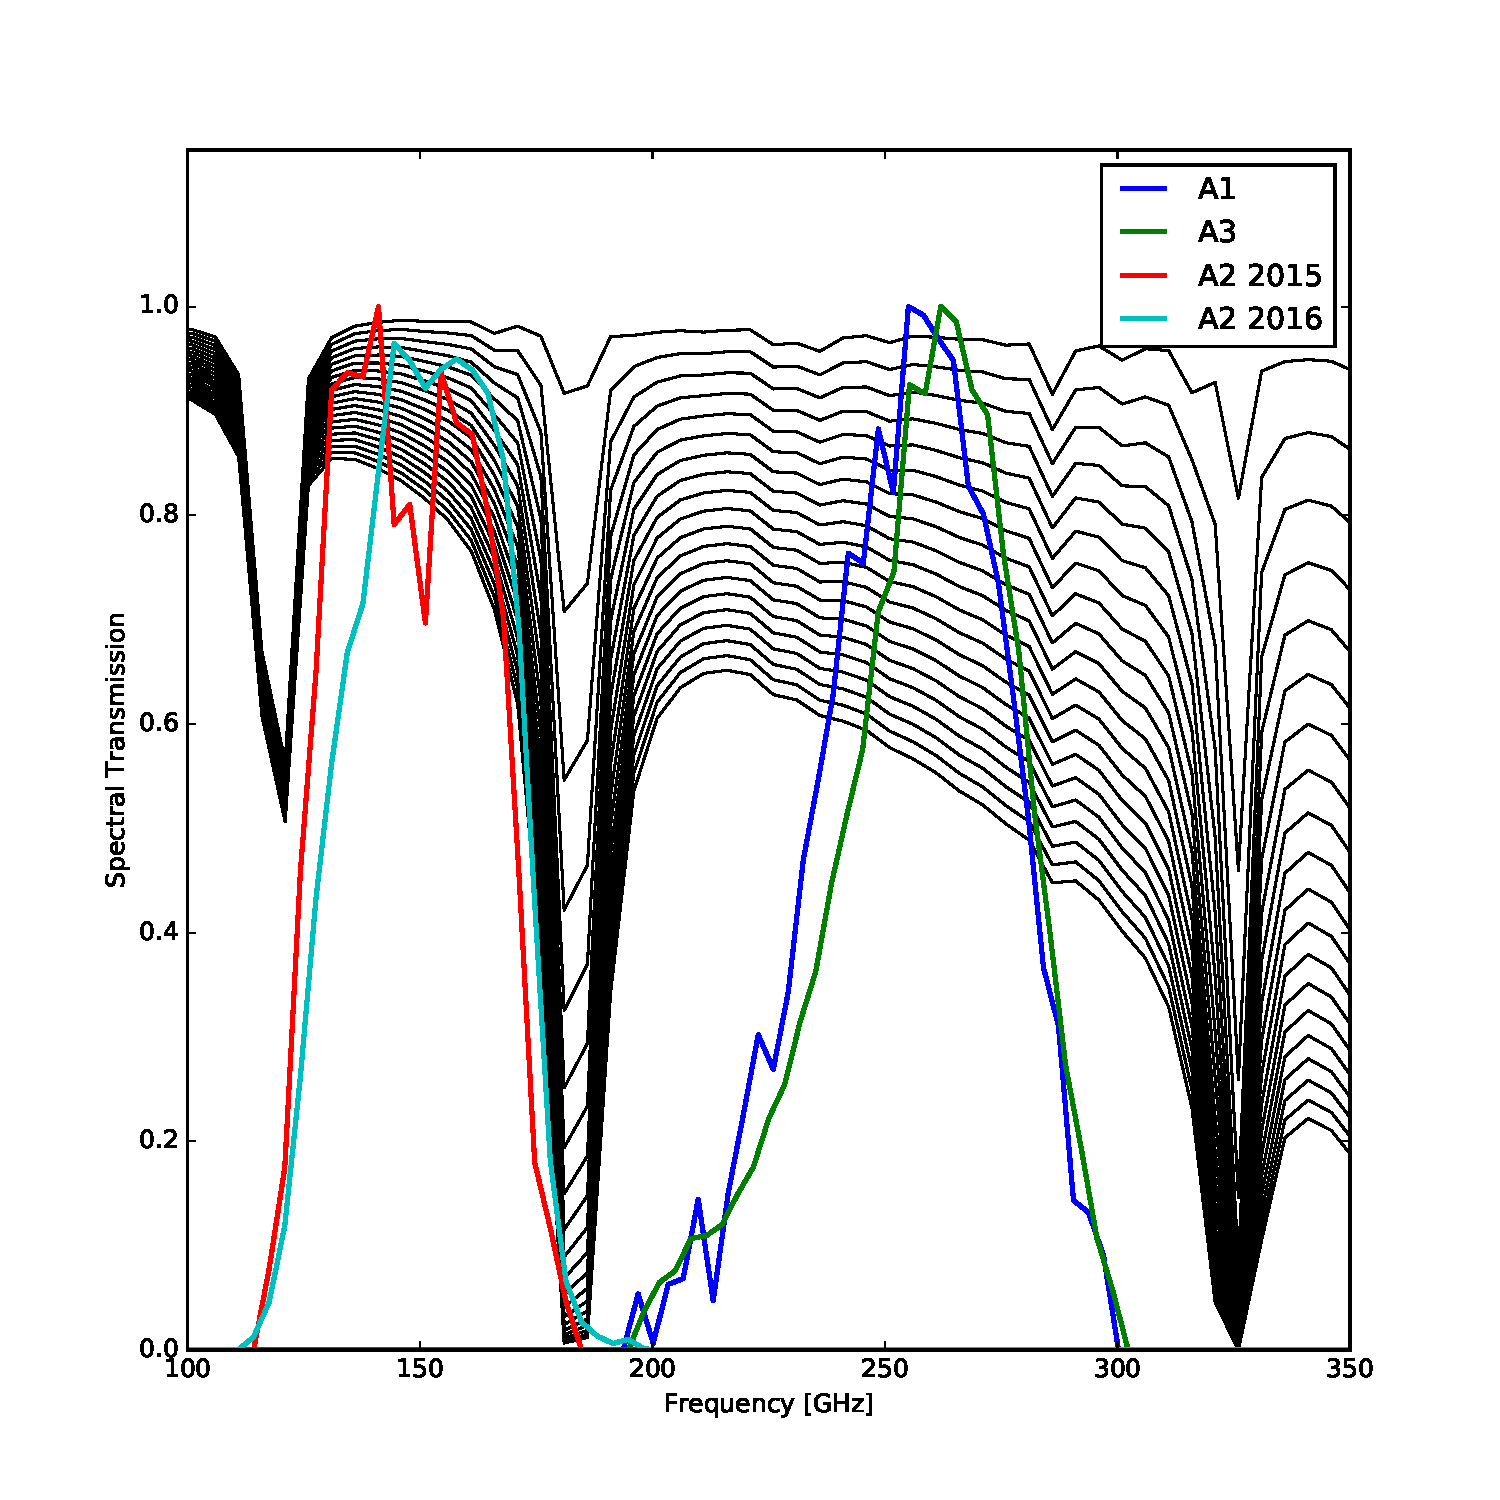
\includegraphics[width=\textwidth]{Figures/SpectralBands/atm_transmission.pdf}
\end{center}
\caption{Spectral transmission of the the three NIKA2 arrays as a function of frequency in GHz. For illustration we also plot the ATM atmospheric model for different values of pwv. \label{spectralband}}
\end{figure}




The NIKA2 spectral bands were measured in the laboratory using a Martin Pupplet interferometer.
Both arrays and filter bands were considered in the measurements. Theser were obtained from the difference of two black-bodies, hence they include a a $\nu^2$ RJ term. During the commissioning in Run 5 array 2 was replaced. The new array has a different spectral transmission. Figure shows the spectral transmissions for the three arrays. Notice that array A2 was replaced by a new on in N2R5 and that the spectral transmissions are not the same (red and cyan lines in the figure).


\begin{table}[h]
\caption{Spectral transmission characteristics for the NIKA2 arrays.%
\label{nika2runs}}
\begin{tabular}{|c|c|c|c|c|}
\hline 
  &     A1  &  A3 &  A2 2015 & A2 2016 \\ 
\hline 
Central Frequency [GHz] &   255.5  & 257.8   &   147.7  & 151.6 \\  
Bandwidth [GHz]         &   47.8   & 45,7    &   41.8   & 42.1 \\
\hline 
\end{tabular} 
\end{table} 


What actually matters more than the ``central frequency'' that depends on many
assumptions and definitions are the bandpasses. We should make available in a
.fits file, clearly, our bandpasses to avoid future misunderstanding and propagation of
false numbers. Official values should be 150 and 260~GHz. We should also clearly
state that these measured bandpasses were done with the difference of two
black-bodies, hence they include a $\nu^2$ RJ term.\\

With these bandpasses and an official ATM spectrum, we expect an opacity ratio of
XX between 1 and 2mm and see~\ref{se:opacities} for more details.





%----------------------------------------------------------------------------------------
%	OPACITY
%----------------------------------------------------------------------------------------
\section{Opacity derivation}
\label{se:opacities}

For each kid $k$, $f_{tone}^k$ moves with the atmospheric load according to

\begin{equation}
f_{tone}^k = C_0^k + C_1^k T_{atm}[1-e^{-\tau/\sin\delta}]
\end{equation}

where $\delta$ is the elevation. The {\tt skydip} procedure consists in moving
the telescope in elevation step by step and to monitor, for each kid, the
evolution of $f_{tone}^k$ vs the air mass and to fit the opacity $\tau$ and
$C_0^k$ and $C_1^k$. All the skydips (that were obtained under various opacity
conditions) are analysed together to break the degeneracies between these
parameters. The procedure has two steps. First, all the skydips are analysed
individually to simply measure $f_{tone}^k$ for each stable elevation and fit
simultaneously all the parameters. Error bars on $\tau$ are estimated by doing
this procedure on blocks of 40 kids only and getting a dispersion on the
resulting $\tau$ from the different blocks. Usually the dispersion comes out as
$4\times 10^{-3}$ at 1mm and $1\times 10^{-3}$ at 2mm. Once the $\tau$ values
are estimated for each skydip (as the average over the blocks), we compute
(while fixing $\tau$) the $C_0$ and $C_1$ final values for each kid. We thus
retrieve the coefficients of all the Kids even though some of them could not
contribute to the tau determination.

%% \begin{figure}
%% \begin{center}
%% 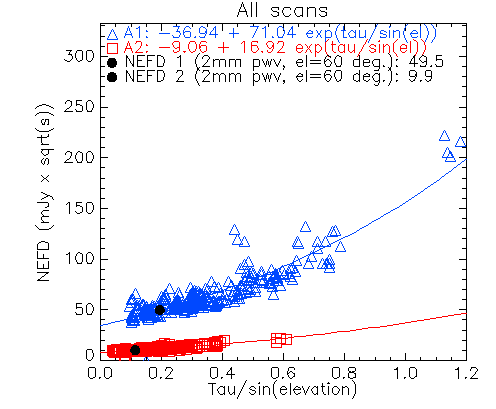
\includegraphics[clip, angle=0, scale =
%%   0.5]{Figures/NEFD_vs_tau_20170226s415_FXDC0C1_Jy_common_mode_kids_out.png}
%% 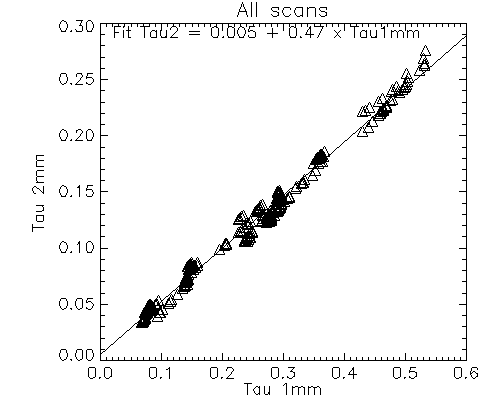
\includegraphics[clip, angle=0, scale =
%%   0.5]{Figures/tau1_tau2_20170226s415_FXDC0C1_GaussPhot_common_mode_kids_out.png}
%% \caption{}
%% \label{fig:fov}
%% \end{center}
%% \end{figure}

\begin{figure}
\begin{center}
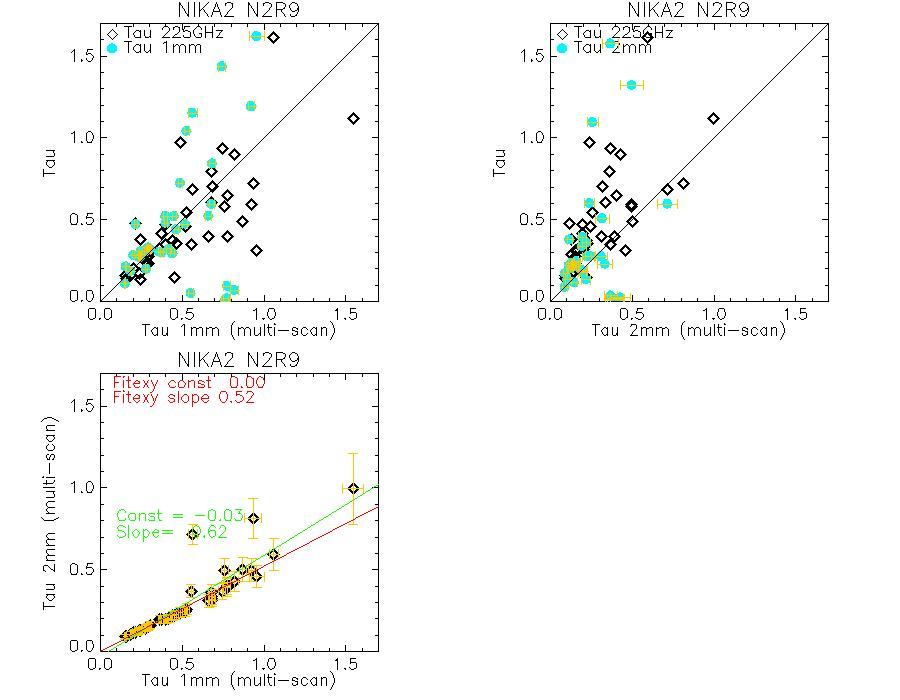
\includegraphics[clip, angle=0, scale = 0.5]{Figures/test_allskd_N2R9.jpg}
\caption{{\bf Fix me : improve plot quality and plot only the 3rd one.}}
\label{fig:test_allskd_N2R9}
\end{center}
\end{figure}


%----------------------------------------------------------------------------------------
%	FOCAL PLANE RECONSTRUCTION
%----------------------------------------------------------------------------------------
\subsection{Methodology}
\label{se:fov}

\begin{figure}[ht]
\begin{center}
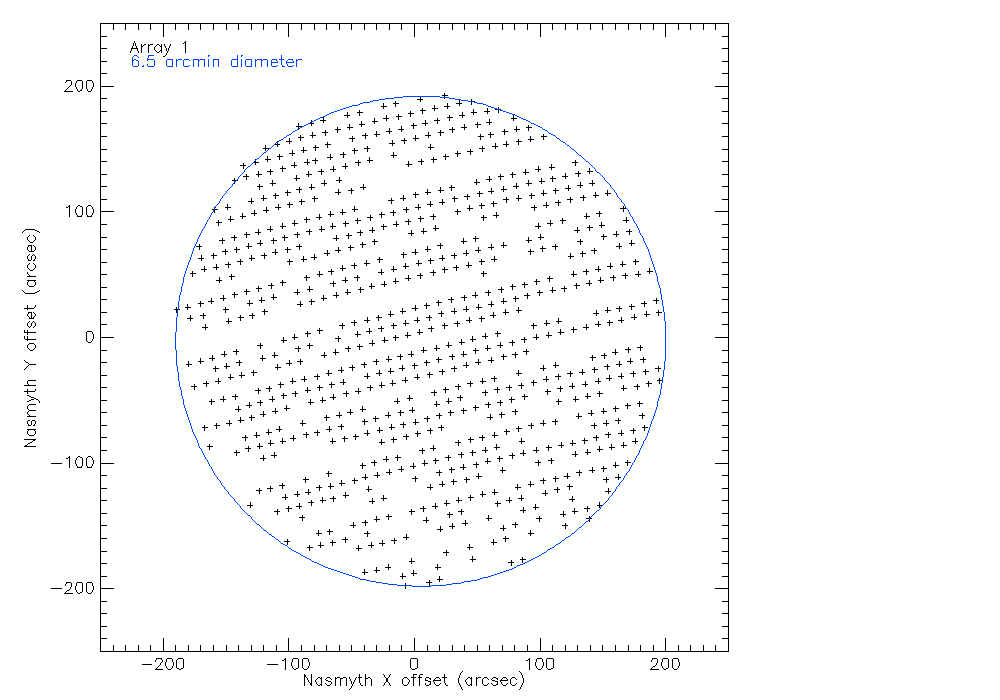
\includegraphics[clip, angle=0, scale = 0.15]{Figures/FOV_A1.png}
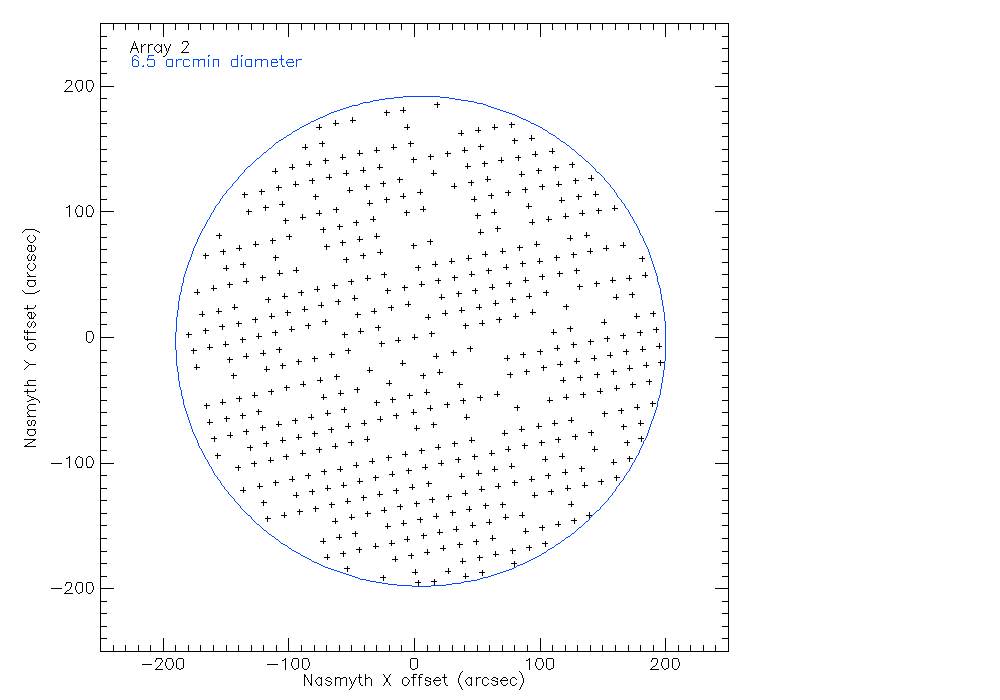
\includegraphics[clip, angle=0, scale = 0.15]{Figures/FOV_A2.png}
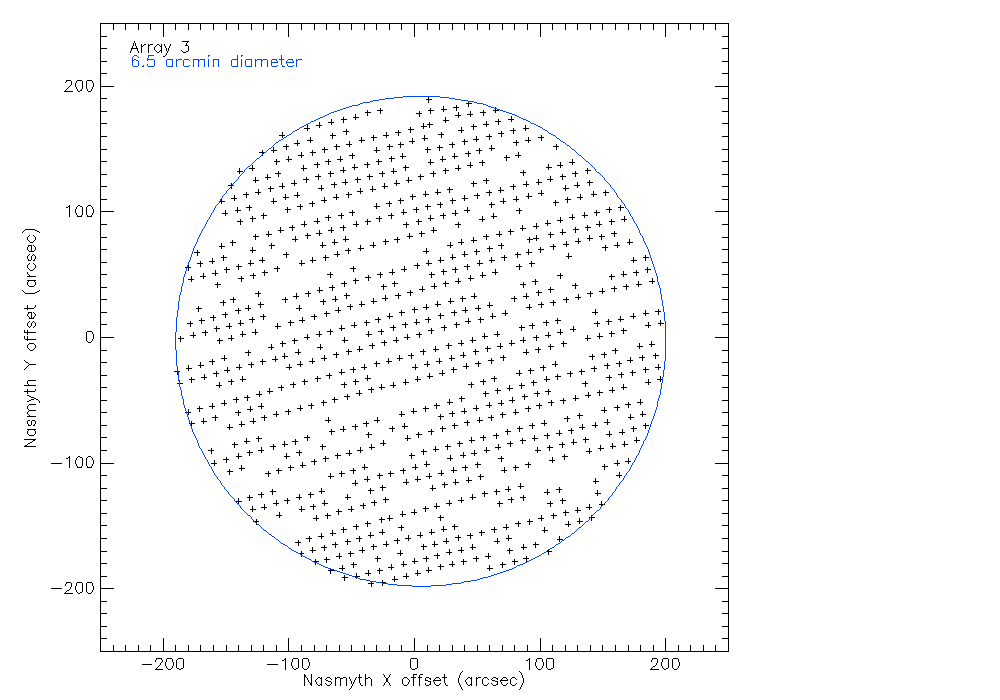
\includegraphics[clip, angle=0, scale = 0.15]{Figures/FOV_A3.png}
\caption{Nasmyth offsets of each array, from beammap 20170226s415 on
  3C84 (N2R9).}
\label{fig:fov_ex}
\end{center}
\end{figure}

% moved to the average FOV section
%\begin{table}
%\begin{tabular}{|l|l|l|}
%\hline
%Array & Number of valid kids & Fraction of all kids\\
%\hline
%A1 & 793 & 0.75\\
%A2 & 481 & 0.83\\
%A3 & 872 & 0.83\\
%\hline
%\end{tabular}
%\end{table}

In order to determine the pointing offsets of each KID w.r.t. the reference sky
coordinates as commanded by the telescope tracking system, we perform a
``beammap'', that is to say we map a bright and compact source, most of the time
a planet, with a elevation step small enough to meet Nyquist sampling at the 1mm
beam scale, namely 4.8~arcsec. We observe this planet with a raster scan in
(az,el) coordinates, either with fixed elevation subscans or fixed azimuth
subscans. The former has the advantage of low air mass variation across a
subscan, the latter offers an orthogonal scan direction to the former: the
combination of both gives a more accurage determination of the far side
lobes. The data reduction proceeds in two steps.

\paragraph{Step 1.} We apply a median filter per
KID timeline whose width is 4~FWHM and we project one map per KID in Nasmyth
coordinates. This median filter removes most of atmospheric and low frequency
electronic noise efficiently, albeit a slight ringing and flux loss on the
source. However, at this stage, we are only interested in the location of the
observed planet. To derive the Nasmyth coordinates from the provided (az,el)
coordinates, we build the following quantities at each time $t$

\begin{eqnarray}
dx_t &=& \cos el_t\, daz_t - \sin el_t\, del_t \nonumber \\
dy_t &=& \sin el_t\, daz_t + \cos el_t\, del_t \nonumber
\end{eqnarray}

where $el_t$ is the elevation of the reference pointing direction and $daz$ and
$del$ are the pointing offsets w.r.t to the source in azimuth and elevation as
provided by the tracking system. Note that $daz$ is already corrected by the
$\cos el_t$ factor to have orthonormal coordinates in the tangent plane of the sky
and be immune to the geodesic convergence at the poles. We then fit a 2D
elliptical gaussian on each kid map. The centroid of this gaussian is a first
estimate of the KID offsets, FWHM's, ellipticity and sensitivity. We apply a
first KID selection by removing outliers to the statistics on these
parameters. We also discard manually KIDs that show a cross-talk counter part on
their map. At the end of this first step, we are ready to move to a second
stage.

\paragraph{Step 2.} With the Nasmyth offsets derived in step 1, we are now able to
mask out the planet in each KID timeline. This mask is centered on the planet
location as seen by each kid, it is circular and has a radius of 60~arcsec. We
now build a template timeline (a.k.a. ``common mode'') in two steps. First, we
take the median of all samples of all KIDs that are outside this mask at a given
time $t$. This gives a first estimate of the common mode. Second, we
cross-calibrate each KID on this common mode when the KID is outside the mask
and we coadd all these KID cross-calibrated timelines when they are outside the
mask to have the final common mode. In this sum, each KID TOI is weighted by the
inverse of its variance outside the mask. Once we have this common mode in hand,
we cross-calibrate each TOI on it outside the mask and we subtract it to the
entire KID TOI. When then resume to the projection of each KID TOI in Nasmyth
coordinates like in step 1, and the 2D elliptical gaussian fit on the each kid
map. The centroid coordinates and the FWHM are now the final parameters that can
be derived on the current scan.

This analysis is repeated on all the beam maps, which provides statistics and
precision on each KID parameter, together with estimates on KID performance stability.

{\bf show a screen capture of Katana.}\\

% LP: j'ajoute une phrase pour referencer la Figure \ref{fig:fov}
We present an example of the FOV reconstruction in Fig.~\ref{fig:fov_ex}.

\begin{equation}
FOV diameter = \sqrt{4 N_{tot. kids} * gridstep^2/\pi}
\end{equation}

{\bf give the values of gridstep (pitch) both in mm and arcsec on the sky}\\

The same definition applies to ``Effective FOV'' to avoid extra multiplication
by the fraction of valid pixels

\begin{equation}
F\lambda = gridstep\times D(30m)/\lambda
\end{equation}



%----------------------------------------------------------------------------------------
%	POINTING
%----------------------------------------------------------------------------------------
\section{Pointing accuracy}
\label{se:pointing}
% + RTA pointing estimate method
% + pointing model
% + pointing error (scan-to-scan scattering)

\begin{figure}
\begin{center}
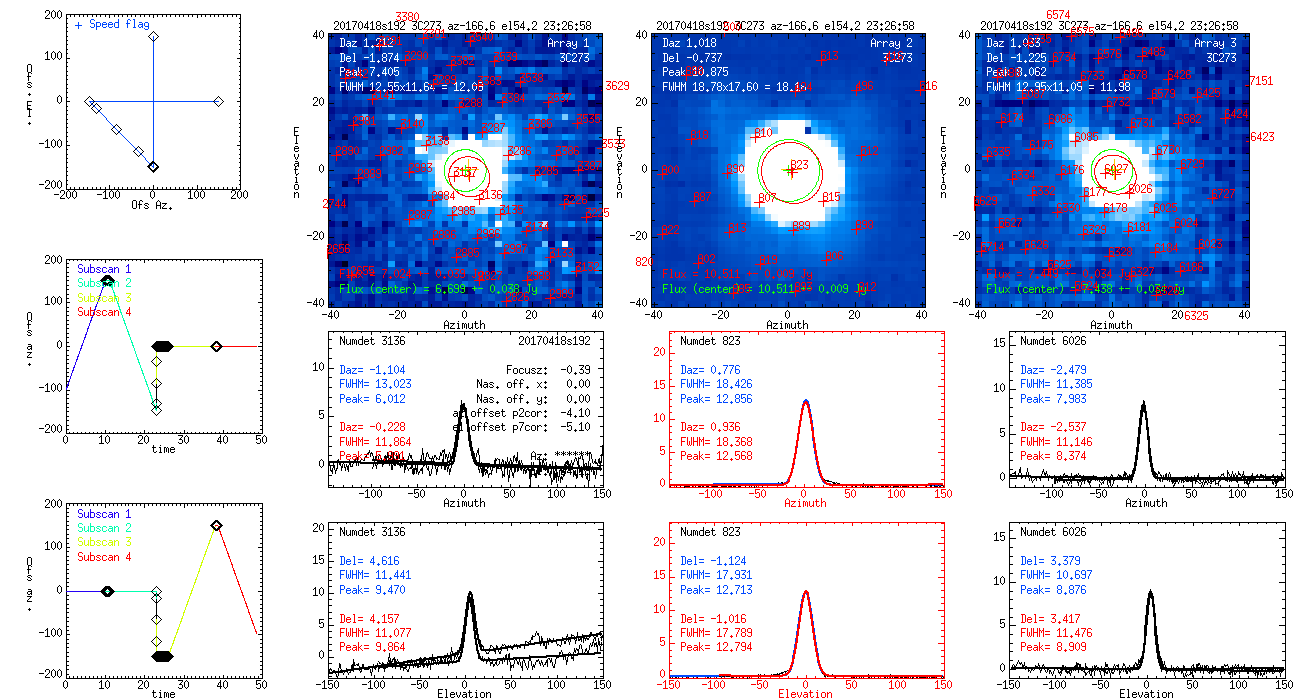
\includegraphics[clip, angle=0, scale = 0.30]{Figures/plot_20170418s192.png}
\caption{Summary plots of the reduction of pointing scan. There is one combined
  map per array to check the overall quality of the scan, and a set of azimuth
  and elevation profiles for one reference detector per array. The 2mm reference
  detector, highlighed in red, is the the pointing reference detector of
  NIKA2. The location of the peak in azimuth and elevation, as observed by the
  reference detector gives the pointing offset of the current scan.}
\label{fig:ptg}
\end{center}
\end{figure}

\begin{figure}
\begin{center}
\includegraphics[clip, angle=0, scale = 0.70]{Figures/pointing_stats_N2R9.eps}
\caption{Pointing offsets during Run9 observations, before and after the
  derivation of Nasmyth offsets with a pointing session on Feb.~26th, 2017.}
\label{fig:pointing_stats_n2r9}
\end{center}
\end{figure}

Based on general operating experience at the 30m telescope, we use the so-called
``pointing'' or ``cross'' scans to monitor the pointing during observations. The
telescope executes a back and forth scan in azimuth and a back and forth scan in
elevation, centered on the observed source. Looking at the timeline profiles of
the reference detector, we fit gaussian profiles and derive the current pointing
offsets of the system in azimuth and elevation. These offsets can then be passed
to PAKO to recenter the next scan (Fig.~\ref{fig:ptg}).

Such scans and their analyses are also used to improve the pointing model
of NIKA2. A pointing session consists in observing about 30 sources on a wide
range of elevations while monitoring the pointing offsets that are measured for
each observation. These offsets and then passed to the IRAM staff who then find
the pointing model parameters that minimize and symetrize the scattering of
these offsets
(cf.~Fig.~\ref{fig:ptg_scattering}). Fig.~\ref{fig:pointing_stats_n2r9} shows
the pointing corrections that had to be applied during Run9, before and after
the derivation of the new Nasmyth offsets. While the absolute values of the
corrections is somewhat arbitrary and set around zero for convenience, the
dispersion of the offsets is the true figure of merit of the pointing
corrections. The distribution of corrections after the corrections (in yellow to
red) is clearly more symetric and narrower than before. The pointing accuracy is
1.62 arcsec rms in azimuth and 1.37 arcsec rms in elevation.



%----------------------------------------------------------------------------------------
%	BEAM PATTERN
%----------------------------------------------------------------------------------------
\section{Beam pattern}
\label{se:beams}
%%
%%
%%      SECTION: BEAM PATTERN 
%%

%% [intro]
%%________________________________________________________

The NIKA2 beam pattern mainly depends on the IRAM 30m telescope and NIKA2 internal optical system characteristics, whereas the detectors themselve might have an impact at sub-dominant level (through e.g. time constants or correlated noises). In this section, first we reconstruct the focus surfaces and present the optimal focus, then we characterize both the main beam, which is modeled as an elliptical Gaussian, and the full beam pattern including error beams up to angular scales of 10 arcmin. 

%% [Optimal Focus]
%%________________________________________________________
\subsection{Optimal focus}

\subsubsection{Focus estimation}

[DESCRIPTION NK-OTF-FOCUS + 1 FIG. D'EXEMPLE]

\subsubsection{Reconstruction of the focus surfaces}

[DESCRIPTION BEAMMAP SEQUENCE + FIGS]


%% [Main beam]
%%________________________________________________________
\subsection{Main beam}

For NIKA2 main beam characterization, we use \emph{Run9} OTF scans of bright point sources, including primary and secondary calibrators. Namely, we consider scans of Uranus, Neptune, 3C273, 3C84, 0316+413, Vesta and MWC349, whereas we avoid CRL2688 and NGC7027, which are slighltly extended. We perform a conservative data selection from the observing conditions by demanding average elevations $\rm{el} \ge 20°$, zenith opacities as estimated by NIKA2 in the 1mm band $\tau_{1\rm{mm}} \le 0.4$, reasonable lateral focus settings $x, y \le 0.5$mm. After selection cuts, our data set includes 130 OTF scans, which consists of a representative sub-sample of a typical NIKA2 observation campaign.    

  
We consider different methods for the main beam characterization: i) Gaussian fits of the beam profile to benefit from the signal-over-noise increase after azimuthally averaging the signal, ii) Elliptical Gaussian fits of the beam map for a better 2D modeling. Cross-checking the outputs from these complementary methods is an important robustess test of our results.   


\subsubsection{profile-based analysis}

[JEAN-FRANCOIS]

\subsubsection{map-based analysis}

NIKA2 main beam two-dimensionnal distribution is modeled using an elliptical Gaussian. We characterize NIKA2 resolution by giving the \emph{FWHM}, defined as
\begin{equation}
  FWHM = 2 \sqrt{2\ln {2}} \sqrt{\sigma_x\sigma_y},
\end{equation}
where $\sigma_x$ and $\sigma_y$ are the Gaussian standard deviation along minor- and major-axis. To avoid the side lobes contamination, we use masked versions of the beam map, in which an annulus of inner radius $r_{\rm{in}}$ and outter radius $r_{\rm{out}}$ is cut out. Whereas $r_{\rm{out}}$ is conservately set to be $100 arcsec$, $r_{\rm{in}}$ can vary to provide the best 2D Gaussian fit. We checked a posteriori that $r_{\rm{in}}$ distributes as $7 \pm 1.5$ arcsec at 1mm and $13 \pm 4$ arcsec at 2mm, in agreement with settings defined in the profile-based analysis.   

Figure~\ref{fig:fwhm_map} shows FWHM distributions obtained from the elliptical Gaussian fit method.


\begin{figure}
\begin{center}
  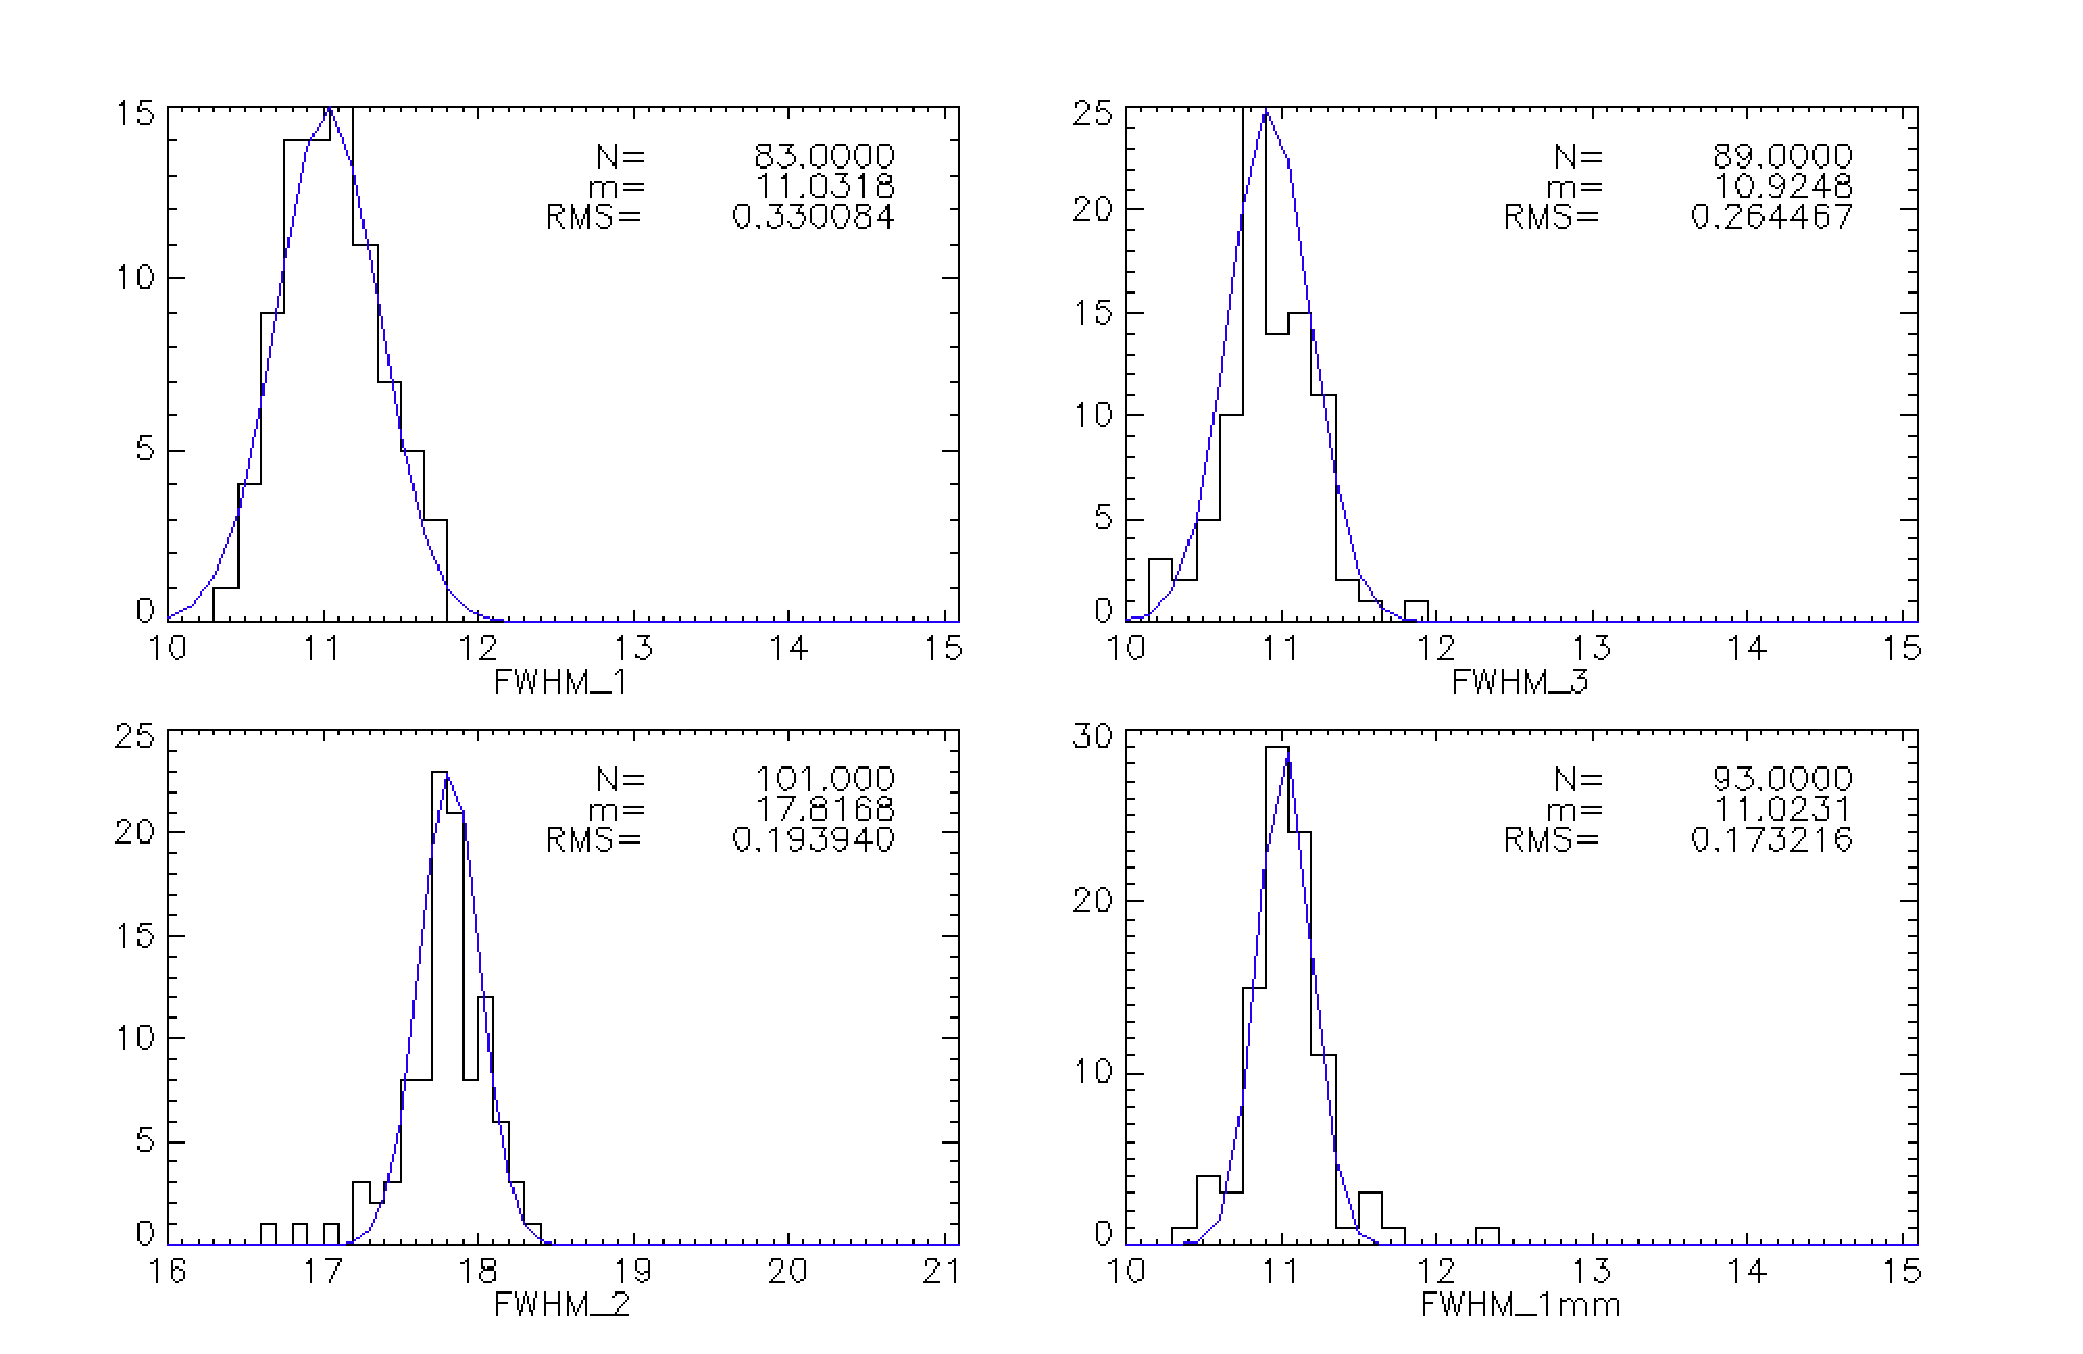
\includegraphics[clip, angle=0, scale=0.4]{Figures/plot_histo_fwhm_run9_calibII_all_nocut.pdf}
\caption{Distribution of the FWHM estimates using 2D Gaussian fits on \emph{N2R9} OTF scans of brigth point sources}
\label{fig:fwhm_map}
\end{center}
\end{figure}


The FWHM estimates using the profile-based and map-based methods are gathered in Tab.~\ref{tab:fwhm}. 
\begin{table}
  \caption[]{FWHM of the NIKA2 main beam in arcsec.}
  \centering
  \begin{tabular}{|l|l|l|l|l|}
    \hline
    Array & profile-based method & map-based method \\
    \hline
    A1       & [TBC] & $11.0 \pm 0.3$ \\
    A3       & [TBC] & $10.9 \pm 0.3$ \\
    A1 \& A3 & [TBC] & $11.0 \pm 0.2$ \\
    A2       & [TBC] & $17.8 \pm 0.2$ \\
    \hline
  \end{tabular}
  \label{tab:fwhm}
\end{table}



%% [Full beam pattern]
%%________________________________________________________
\subsection{Full beam pattern}

\subsubsection{Deep beam maps}
We present the two-dimensional distribution of the beam in Fig.~\ref{fig:beam}. We primary use a map obtained from a combination of deep observations of strong point sources collected during \emph{NIKA2-run8} and \emph{run9}. Namely, we use 'beammap' OTF scans of Uranus (scan id '20170125s223' and '20170125s243'),  Neptune ('20170224s177') and the bright quasar 3C84 ('20170226s415'). However, we checked the stability of our results on single scan maps, combinations of scans for a single source, and combinations of shallower scans but spanning a large range of scanning direction. The data processing includes a mitigation of the correlated noise, which mainly originates from the atmosphere.  We primarly use a subtraction of a common mode estimated from the most correlated detectors (the so-called 'cm one block' method). However, other methods are tested for assessing the immunity of our results to noise residuals.

\begin{figure}
\begin{center}
  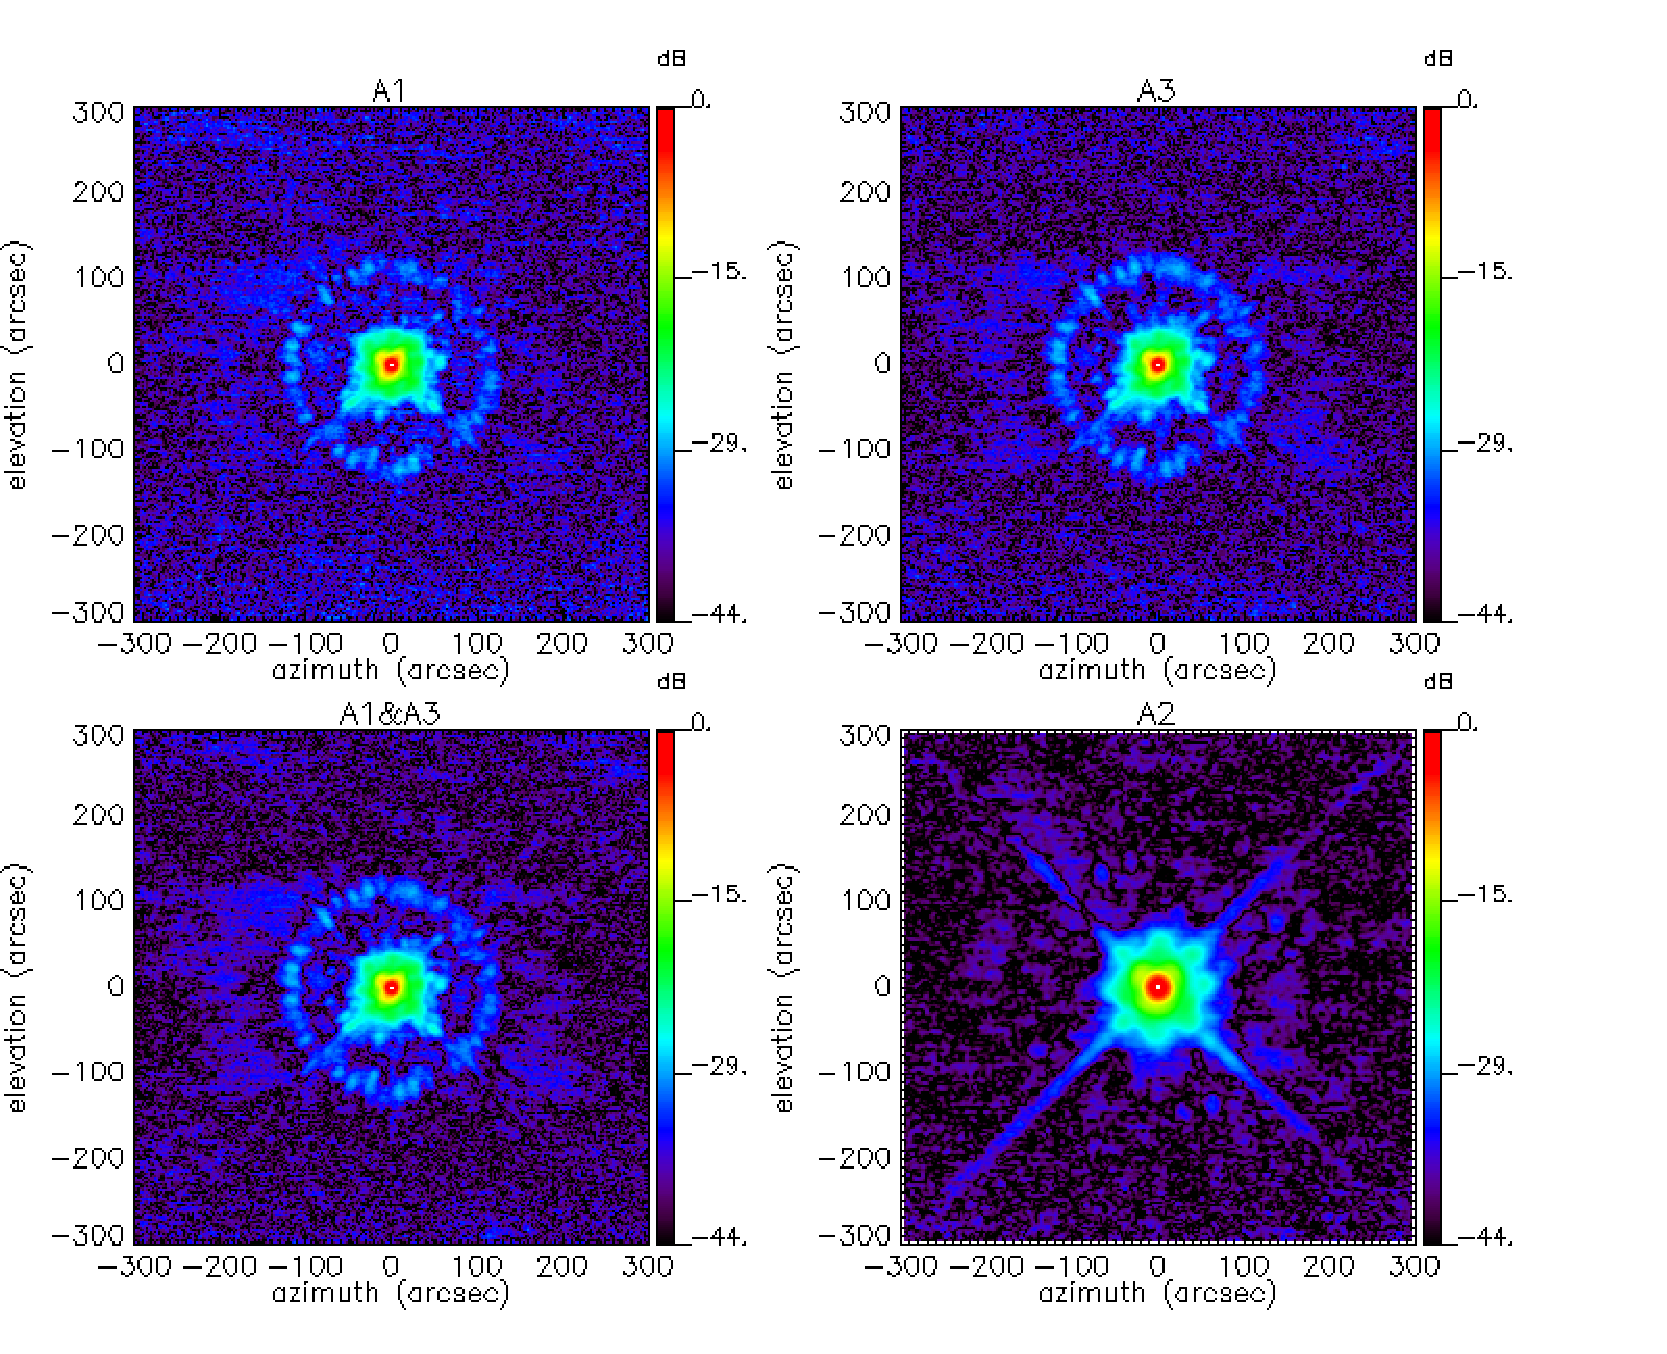
\includegraphics[clip, angle=0, scale=0.4]{Figures/Lobe_map_Combo_v2_dB.pdf}
 \caption{Beam pattern. From upper left to lower right, beam maps of array 1 (labeled 'A1'), array 3 ('A3'), the combination of the 1.15mm arrays ('A1$\&$3') and the 2mm array ('A2') are shown in decibel. These maps, which consist of normalized combination of four long OTF scans of bright point sources, are in celestial coordinates and cover a sky area which extend over 10 arcmin.}
\label{fig:beam}
\end{center}
\end{figure}


The deep NIKA2 beam maps reveal some noticeable features, which are shown in Fig.~\ref{fig:features}. 

\begin{figure}
\begin{center}
  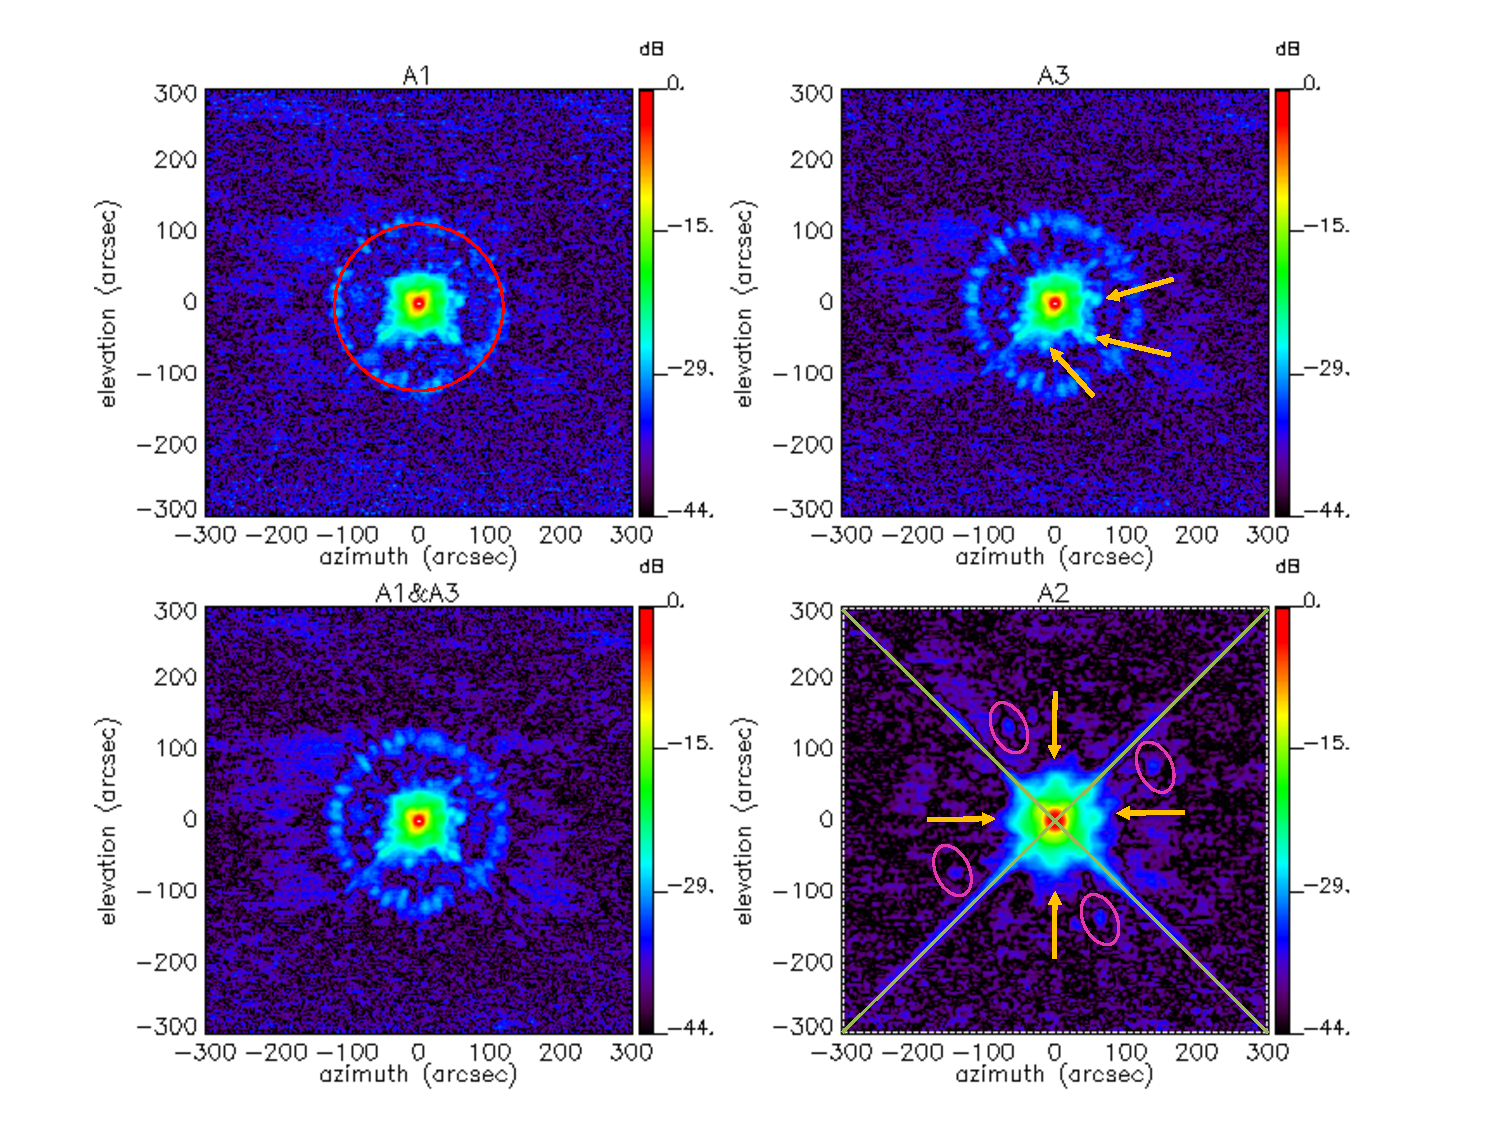
\includegraphics[clip, angle=0, scale=0.4]{Figures/Beams_features.pdf}
\caption{Noticeable features of NIKA2 beam pattern. Red circle: diffraction ring seen in 1-mm maps (the spokes are presumably caused by radial and azimuthal panel buckling (cf. Fig.4 in Greve et al. 2010)); Perpendicular green lines: diffraction pattern caused by quadrupod secondary support structure (prominently seen in 2mm maps); Yellow arrows in the upper right pannel: pattern of 3 spikes seen in 1mm maps of unknown origin; Yellow arrows in the lower right pannel: four symmetrical spokes of the first errorbeam; Pink ellipses: 4 spikes seen in 2mm maps.}
\label{fig:features}
\end{center}
\end{figure}

We further quantify the relative level of the main beam, the first error beam and other features seen in the 2D beam pattern using radial cuts.

[FIGURE JEAN-FRANCOIS]

\begin{figure}
\begin{center}
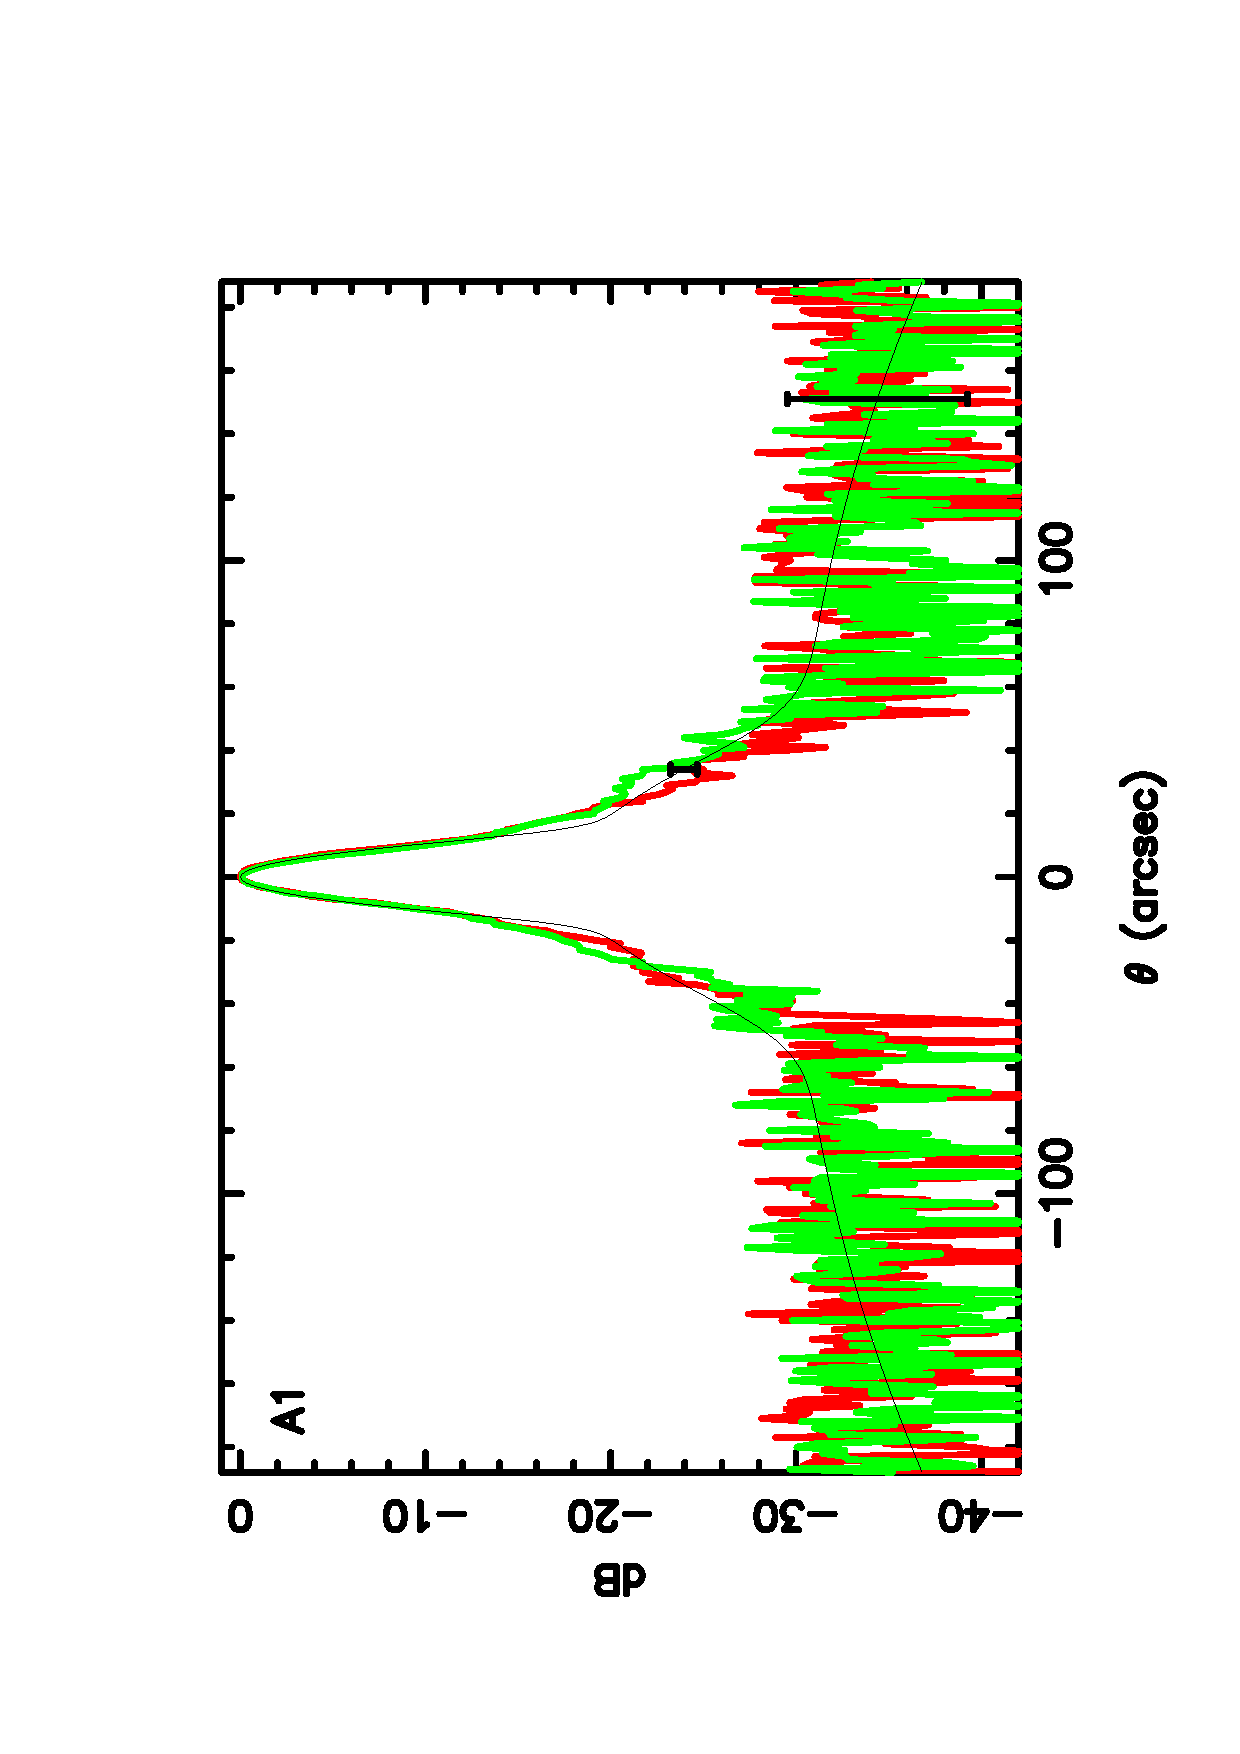
\includegraphics[clip, angle=-90, scale =0.3]{Figures/Array_A1_dB.pdf}
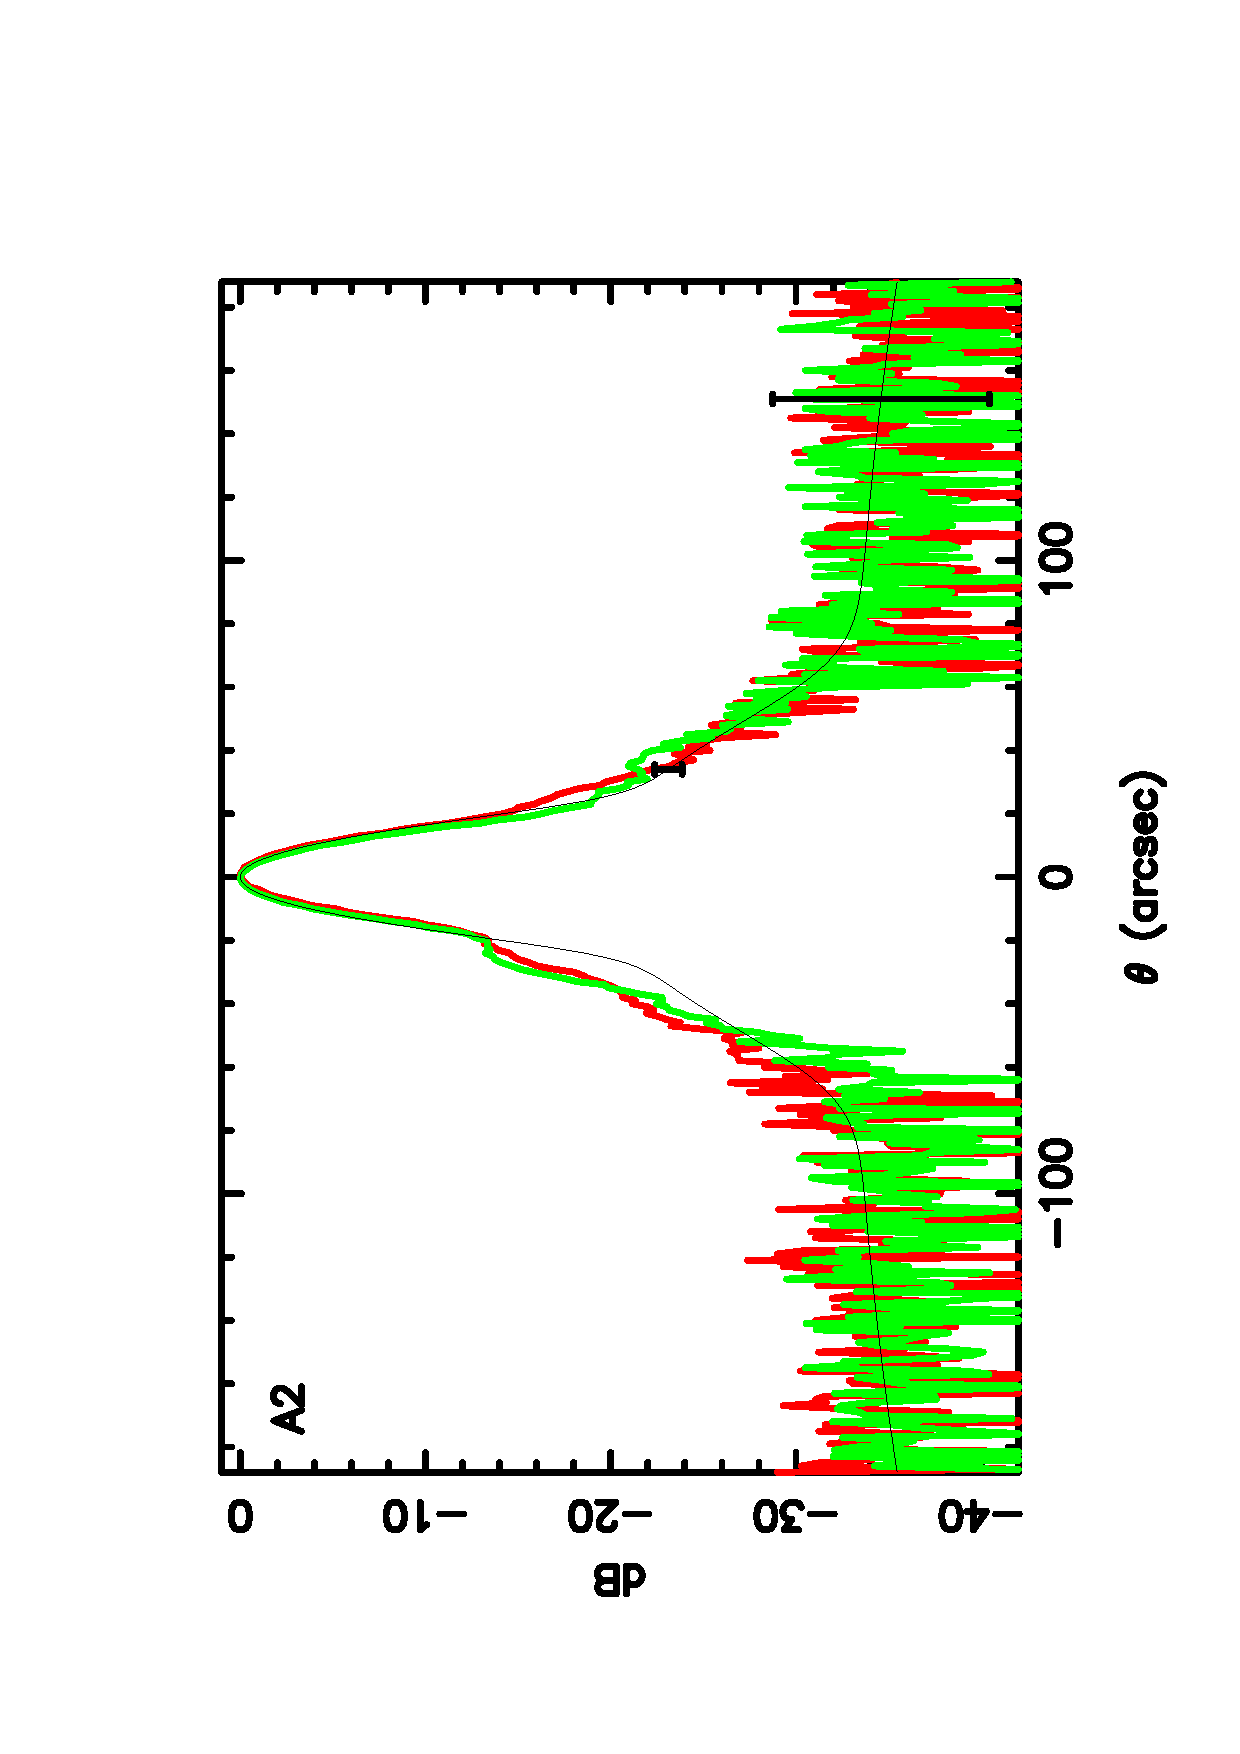
\includegraphics[clip, angle=-90, scale = 0.3]{Figures/Array_A2_dB.pdf}
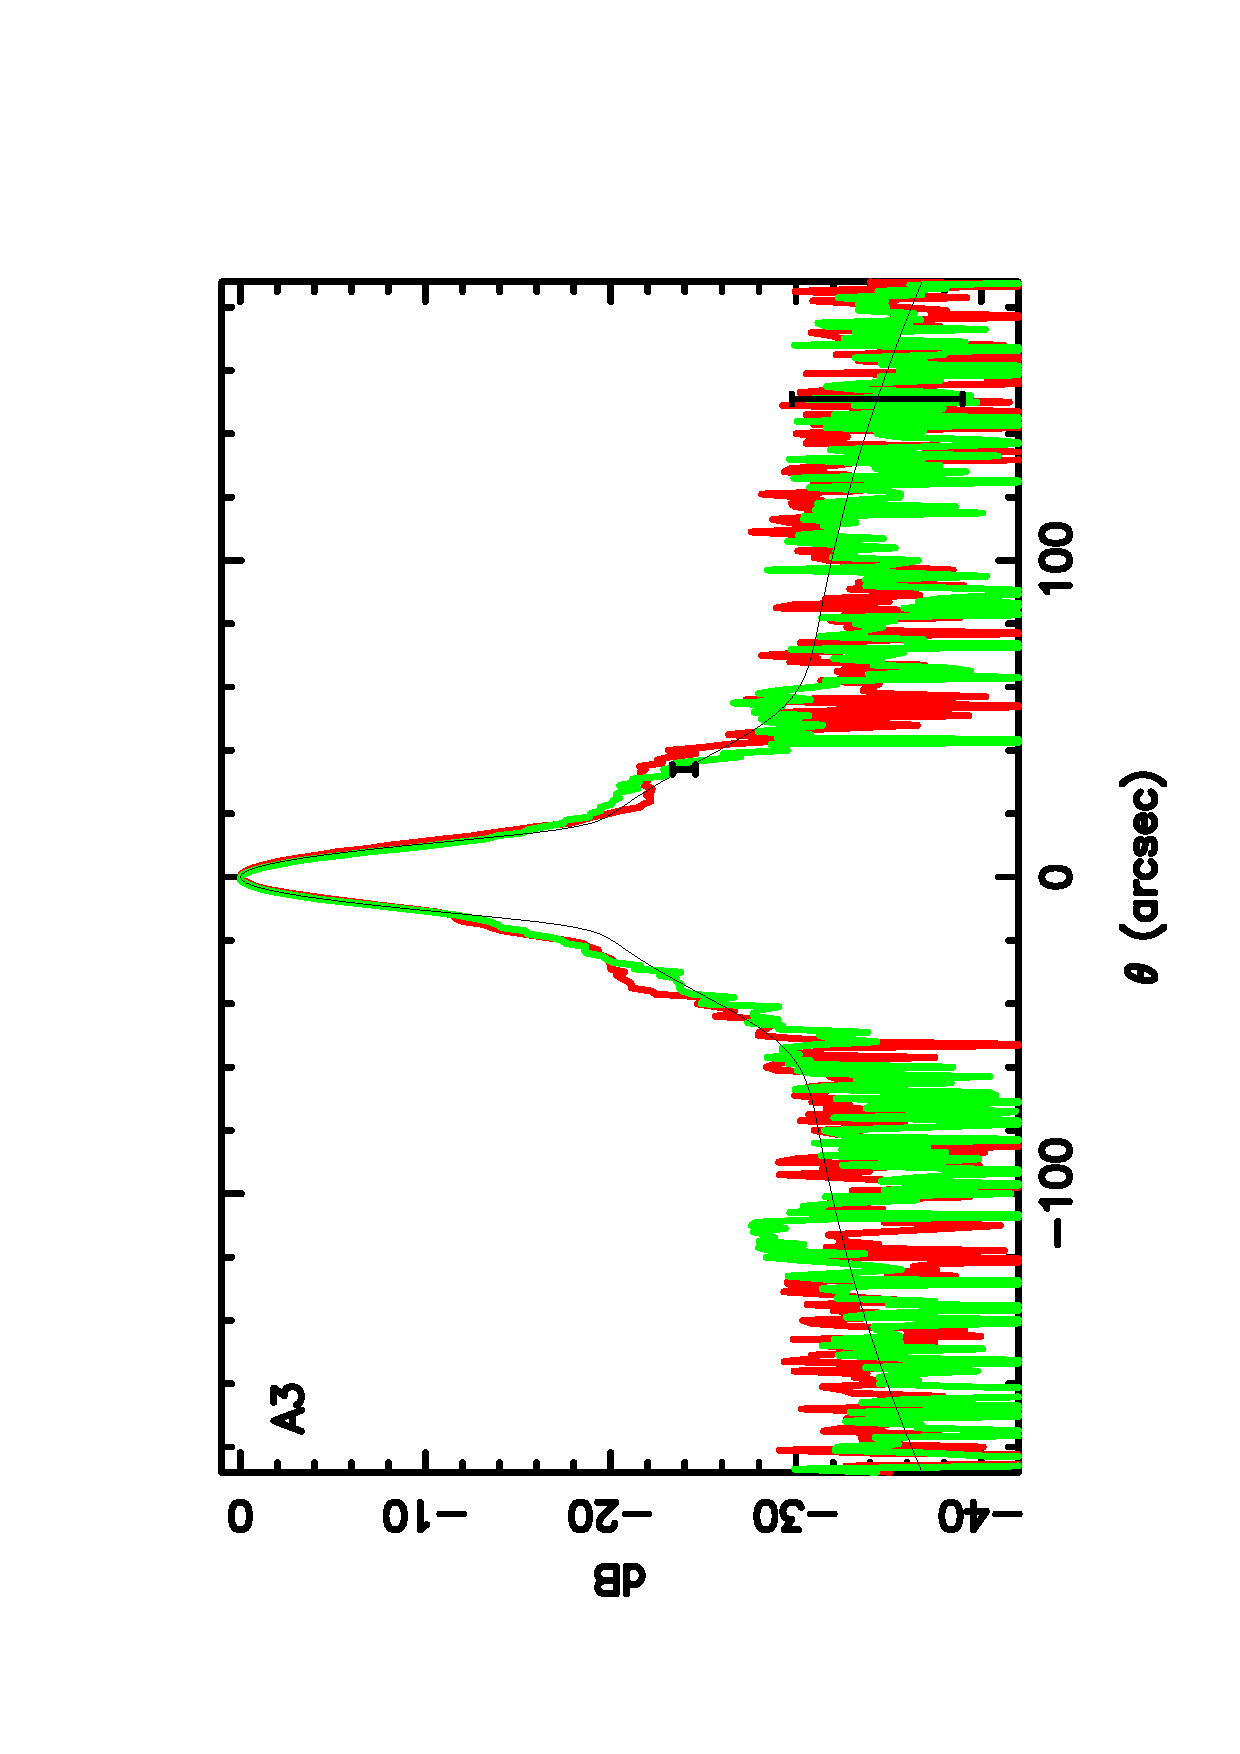
\includegraphics[clip, angle=-90, scale = 0.3]{Figures/Array_A3_dB.pdf}
\caption{Two orthogonal cuts through the beam are shown in red and green and a best fit model made
of three Gaussians is superimposed in black. These cuts were obtained from the high quality map of Uranus on 2017 January 25th.
The main beam starts to depart from the first Gaussian at -12dB. }
\label{fig:beam_dB3}
\end{center}
\end{figure}

The Iram 30-m beam as seen with NIKA2 is shown in
Fig. \ref{fig:beam_db} by means of two orthogonal cuts through Uranus
from a high quality map obtained on 2017 January 25th in excellent conditions
(low opacity $\tau_{225}=0.08$ and elevation $46^{\circ}$).
A model made of three Gaussians centered on the source peak was best
fit {\it by hand} to these cuts and the parameters are reported in
Table \ref{tab:3gauss} [PEUT-ETRE AVANTAGEUSEMENT REPLACED PAR VALEURS DE FLORIAN].
The main beam starts to depart from the first
Gaussian at the level of about -12dB for the three arrays.
We note that for the instrument EMIR on the radiotelescope,
this departure is about -20dB (Kramer, Penalver and Greve 2013).
From parameters in Table \ref{tab:3gauss}, one can estimate that
the source incident power is split about equally between the main beam
and the error beam at 1mm, and these fractions are 70\% and 30\% at 2mm, respectively.
This modelling uses the central
region   $180'' \times 180''$ in size with a uniform noise rms from
a larger area of 8' x 5' on the sky scanned with the arrays. It is expected
that the error beam extend beyond these limits.


\begin{table}
\centering 
\caption[]{Model parameters of the three Gaussian beam.}
\begin{tabular}{|l|l|l|l|l|l|l|}
\hline
               & \multicolumn{3}{c|}{A1 and A3} & \multicolumn{3}{c|}{A2}  \\
\hline
fwhm      & $11.25''$ & $45''$  & $250''$ & $17.75''$ & $56''$  & $420''$ \\
amplitude & 0.984     & 0.015   & 0.0005   &  0.9875   & 0.011   &  0.0005\\
\hline
\end{tabular}
\label{tab:3gauss}
\end{table}


\subsubsection{Beam profile}

\begin{figure*}[h!]
\centering
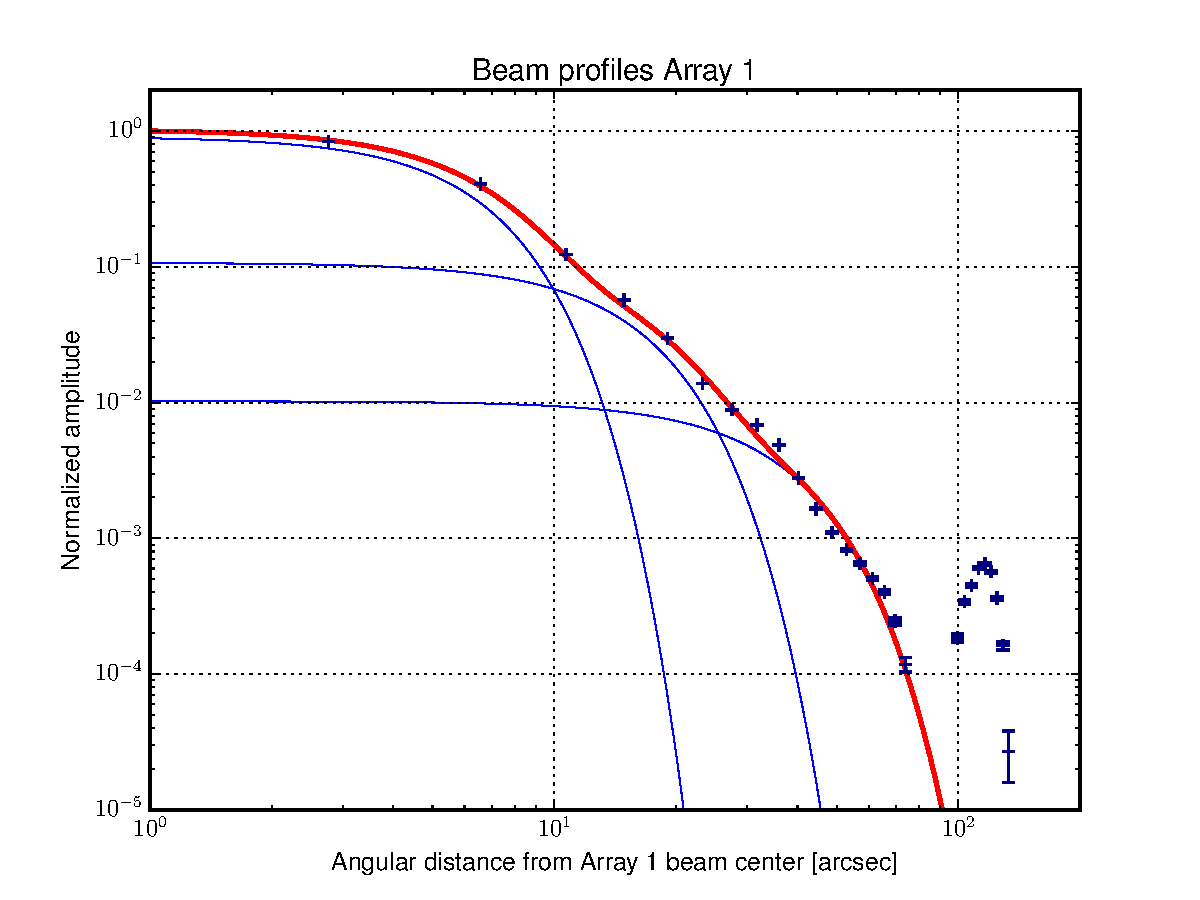
\includegraphics[height=6cm]{Figures/Beam_profiles_A1_FR.pdf}
\hspace{0.5cm}
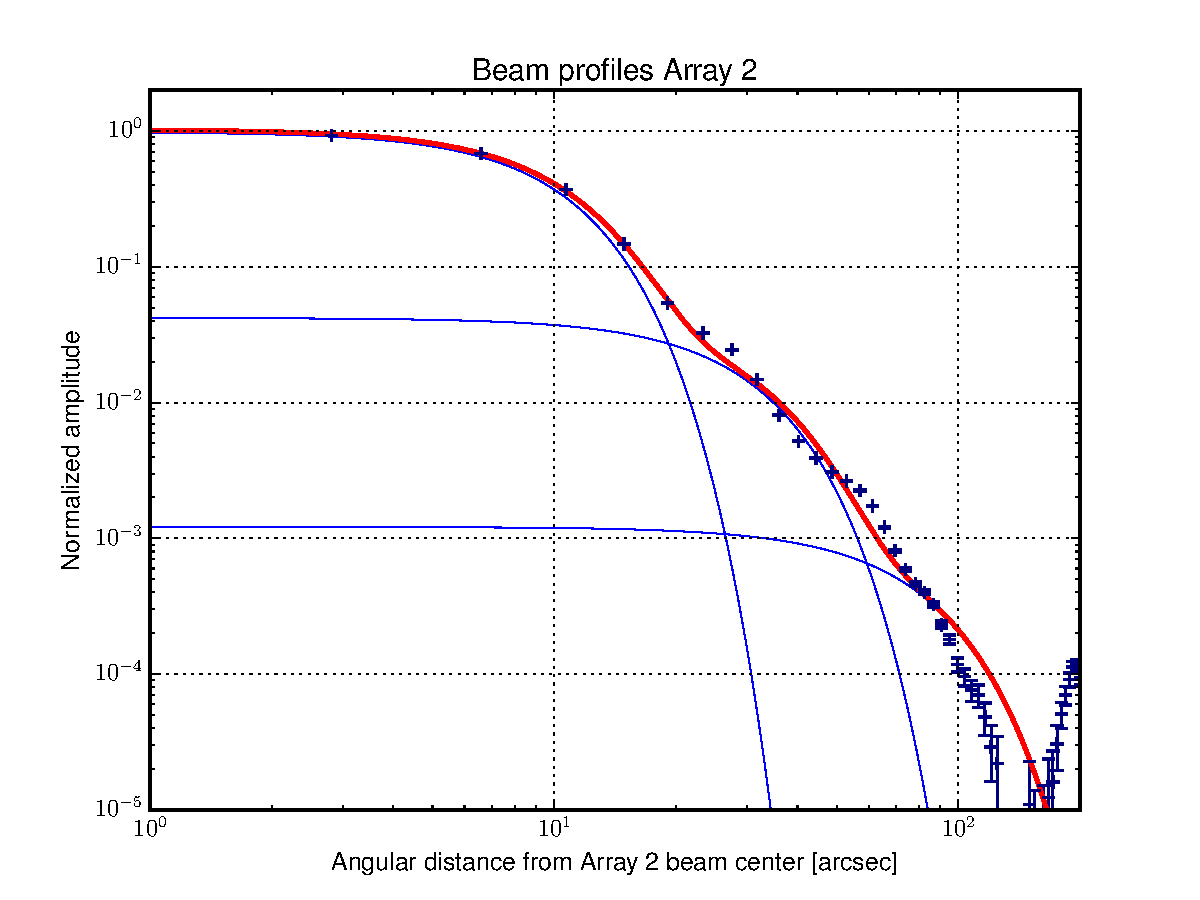
\includegraphics[height=6cm]{Figures/Beam_profiles_A2_FR.pdf}
\hspace{0.5cm}
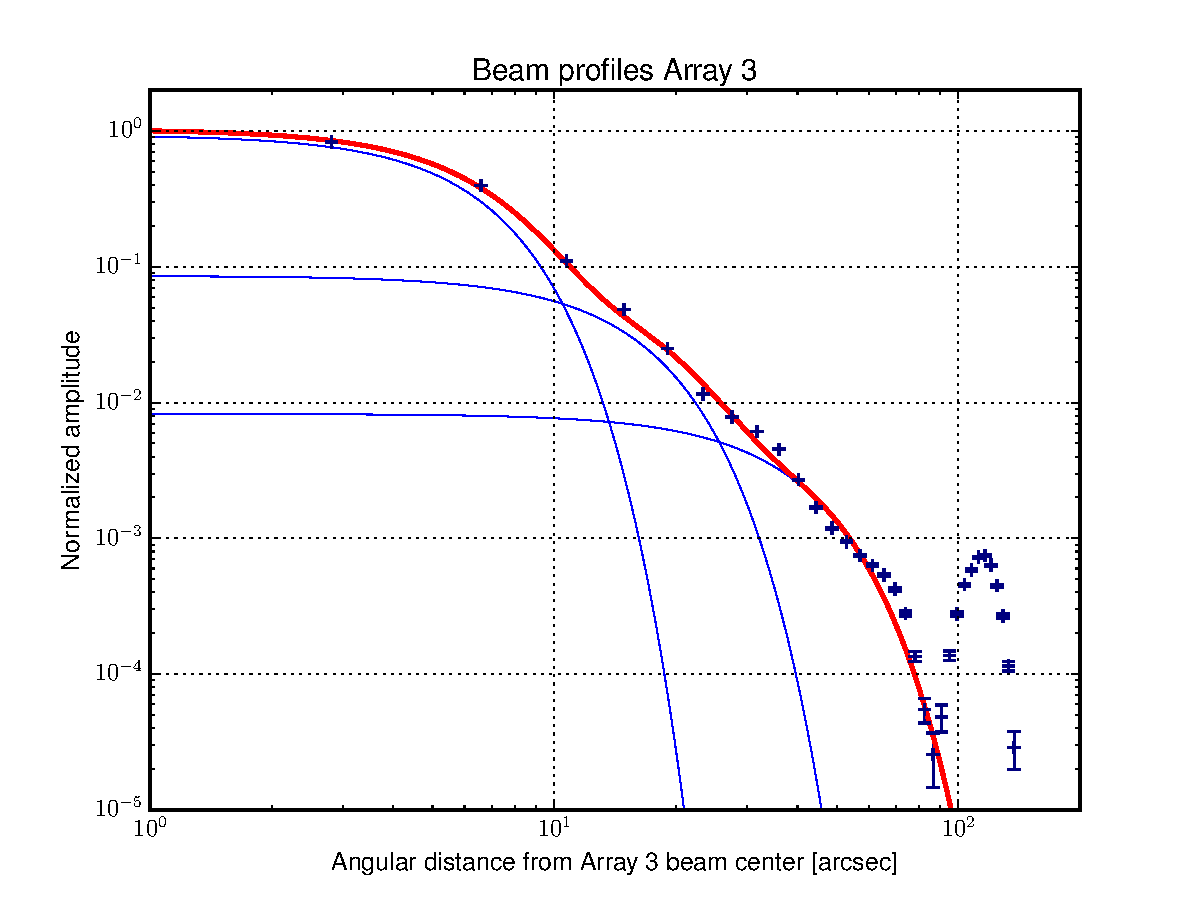
\includegraphics[height=6cm]{Figures/Beam_profiles_A3_FR.pdf}
\caption{{\footnotesize Beam profiles for array 1, 2, and 3.}}
\label{fig:beam_profiles_3G}
\end{figure*}


\subsubsection{Beam efficiency}


%% [STABILITY]
%%________________________________________________________
\subsection{Stability of the beam pattern}

[A FAIRE:

  AJOUTER LES PLOTS DE STABILITE EN FONCTION DE ELEVATION, TAU

]






%----------------------------------------------------------------------------------------
%	CALIBRATION
%----------------------------------------------------------------------------------------
\section{Calibration}
\label{se:calibration}

%
%%
%%
%%

%% [intro]

The calibration of the instrument NIKA2 in its final configuration
of January 24th 2017  is studied in this section  in using the 
 primary calibrators, Uranus and Neptune, and secondary calibrators ; the two largest asteroids Ceres and Vesta, and the three
planetary nebulae NGC7027, CRL2688, and MWC349.

% HA 
\subsection{NIKA2 Photometric System}


\begin{table}[h]
\begin{center}
\begin{tabular}{|c|c|c|}
\hline
     & 1mm & 2mm \\
\hline
Reference frequency $\nu_{0}$ & 260 GHz & 150 GHz \\
\hline
Reference FWHM                      & 12.5  '' & 18.5 '' \\
\hline
\end{tabular}
\caption{NIKA2 reference frequencies and FWHM}
\end{center}
\label{tab:definitions}
\end{table}

\subsubsection{Response of a detector to astronomical source}


Let us consider a source observed at airmass $\sec z$ under
$mm_{H_{2}O}$ of precipitable water, with specific intensity $I_{\nu}$ (in units
of  $W/m^{2}/sr/Hz$) in the direction $\theta, \phi$, where $\theta$
is the off-axis distance and $\phi$ the position angle, illuminating a KID
of the NIKA2 array. 

A KID response located at position $\theta, \phi$
on the focal plane to this signal will be:
\begin{equation}
R(\theta, \phi, \sec z, mm_{H_{2}O}) = G_{k} \int_{0}^{+\infty} I(\nu)
\frac{T'(\nu)}{\left(\frac{\nu}{\nu_{0}}\right)^{2}} e^{\left(-\sec z
  . \tau(\nu,  mm_{H_{2}O})\right)}A\Omega (\nu)  d\nu 
\label{eq:basicphot}
\end{equation}

where the different factors in the integral are:
\begin{itemize}
\item $\frac{T'(\nu)}{\left(\frac{\nu}{\nu_{0}}\right)^{2}}$:  the
  system transmission. $T'(\nu)$ is the transmission as measured in
  section~\ref{se:bandpasses} with a Rayleigh-Jeans source. It is
  divided by $\left(\frac{\nu}{\nu_{0}}\right)^{2}$ to correct for the
  incident spectrum.
\item $e^{\left(-\sec z . \tau(\nu,  mm_{H_{2}O} )\right)}$: the
  atmospheric transmission at airmass  $\sec z$ for an amount of
  precipitable water vapor $mm_{H_{2}O}$ generating an opacity $\tau(\nu)$.
\item $A\Omega (\nu) $: the KID etendue, {\it i. e.} the product of
  its light collecting area by the solid angle it intercept on the
  sky. While the step between  pixels is well known and is measured (see sec~\ref{se:fov}), the
  actual solid angle is not known precisely and is {\em probably} a function of the
  frequency  because the pixels sizes are close to the wavelength of
  operation (2.75 mm at 2mm for example). The collecting $A$ area is the
  projection of the IRAM primary on the cold pupil and is also not
  known very accurately.
\end{itemize}
The integral in eq~\ref{eq:basicphot} gives the total power (units of $W$)
falling on a pixel. The factor $G_{k}$ (units of  $W^{-1}$) convert this
power to ADU. 

By virtue of the conservation of specific intensity in a telescope,
equation~\ref{eq:basicphot} can be rewritten as:
\begin{equation}
R(\theta, \phi, \sec z, mm_{H_{2}O}) = G_{k} A_{pupil}\Omega_{s}\int_{0}^{+\infty} I(\nu)
\frac{T'(\nu)}{\left(\frac{\nu}{\nu_{0}}\right)^{2}} e^{\left(-\sec z
  . \tau(\nu,  mm_{H_{2}O})\right)} \Omega_{beam} (\theta, \phi, \nu)  d\nu 
\label{eq:basicphot2}
\end{equation}
where:
\begin{itemize}
\item $A_{pupil}$ is the area of the entrance pupil ({\it i.e.} the
  dish collecting area).
\item $\Omega_{s}$ is the solid angle of the source seen from the
  entrance pupil.
\item $\Omega_{beam}(\theta, \phi, \nu)$ is the fraction of source signal
  illuminating the KID. It has no units and it is thus normalized so that:
\begin{equation}
\int\int_{4\pi} \Omega_{beam}(\theta, \phi, \nu) \sin \theta d\theta
d\phi = 1 
\label{eq:omegabdef}
\end{equation}
\end{itemize}

Equation~\ref{eq:basicphot2} describe the response of a KID, and it
is quite complex. We will in the following simplify it by making a few
assumptions. Let us first turn ourselves toward the effect of the
atmosphere. 


\subsubsection{Effect of the atmosphere}

In order to study the effects of the atmosphere, let us define the
effective frequency of a source as the weighted frequency of the
passband, taking into account the system and atmospheric transmission,
as well as the shape of the incident spectrum:
\begin{equation}
\nu_{eff}( \sec z, mm_{H_{2}O}) = \frac{ \int_{0}^{+\infty} I(\nu) \frac{T'(\nu)}{\left(\frac{\nu}{\nu_{0}}\right)^{2}} e^{\left(-\sec z
  . \tau(\nu,  mm_{H_{2}O})\right)} \nu d\nu } { \int_{0}^{+\infty} I(\nu) \frac{T'(\nu)}{\left(\frac{\nu}{\nu_{0}}\right)^{2}} e^{\left(-\sec z
  . \tau(\nu,  mm_{H_{2}O})\right)}  d\nu}
\label{eq:nueff}
\end{equation}
In order to compute the atmospheric tramission, we have used
the IRAM atmosphere 2009 models provided in GILDAS, computed for
'midlatwinter' conditions, a temperature of 268 K  and a pressure of 703.5
hPa. $\nu_{eff}$ allows to characterise the impact of the variation of
the atmospheric transmission on the full system transmisison.  Note
that the instrument transmission $T'(\nu)$ is the one measured in
sec~\ref{se:bandpasses}. 

Figure~\ref{fig:nueff} shows the variations of
$\nu_{eff}$ as a function of the water content of the atmosphere for
two elevations (zenith and 20 degree) and two spectral shape (RJ and
flat spectrum), in the two 1mm passbands and in the 2mm passband. 

Typical variations of $\nu_{eff}$ with the spectral shape of the
source range between 1\% and 3\%, and are relatively stable between good
($\tau_{225GHz} \simeq 0.1$) and
poor  ($\tau_{225GHz} \simeq 1.0$) atmospheric conditions for both the
1mm and 2mm bands. 


Let us now examine the effect of elevation.
Under good atmospheric conditions ($\tau_{225GHz} \simeq 0.1$), $\nu_{eff}$ change by
less than 0.3\% betwen zenith and 20 degree elevation. Under poor
conditions ($\tau_{225GHz} \simeq 1.0$), this rises to almost 3\% for
a Rayleigh-Jeans spectrum in the 2mm band, {\it i.e.} larger than the
  variations due to the spectral shape of the source.



\begin{figure}[h]
\begin{tabular}{cc}
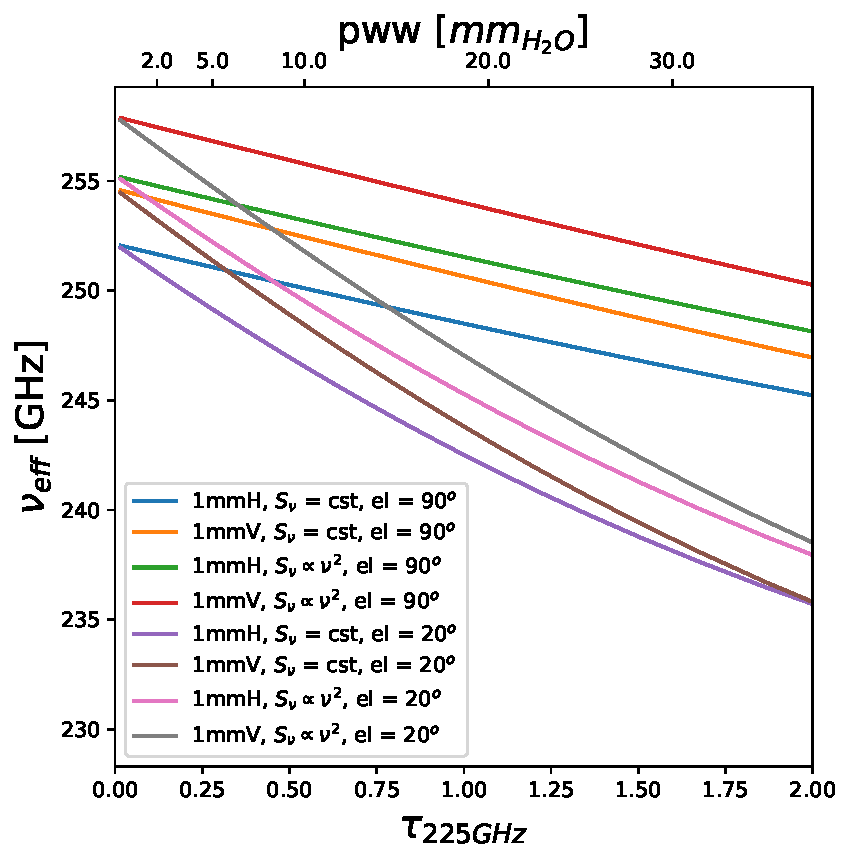
\includegraphics[width=0.5\textwidth]{Figures/atm_nueff_1mm.pdf}
  & 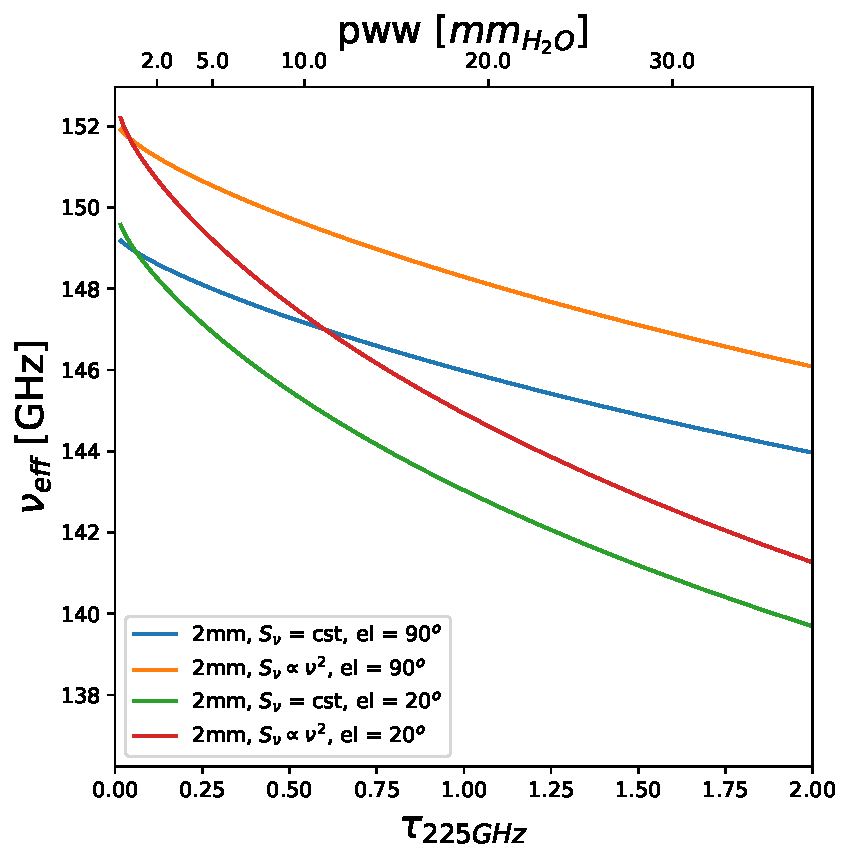
\includegraphics[width=0.5\textwidth]{Figures/atm_nueff_2mm.pdf}
  \\
a) 1mm & b) 2mm \\
\end{tabular}
\caption{Effective frequency as a function of the sky opacity. The
  effective frequency (see text) have been computed for two source
  spectra (RJ and constant), and for two elevations.}
\label{fig:nueff}
\end{figure}

Nevertheless, to a first approximation, we consider the shape of the atmospheric
transmission independent of the elevation and water content, so that  an
effective zenith opacity $\tau_{eff}$
used. 
Equation~\ref{eq:basicphot2} becomes under this assumption: 
\begin{equation}
R(\theta, \phi, \sec z, mm_{H_{2}O}) \simeq G_{k}  A_{pupil}\Omega_{s} e^{\left(-\sec z
  . \tau_{eff}(mm_{H_{2}O})\right)} \int_{0}^{+\infty} I(\nu)
\frac{T'(\nu)}{\left(\frac{\nu}{\nu_{0}}\right)^{2}} T_{atm}(\nu)
\Omega_{beam} (\theta, \phi, \nu) d\nu 
\label{eq:basicphot3}
\end{equation}
where $T_{atm}(\nu)$ is the transmission of the atmosphere at zenith,
and is a function of the frequency only. From the computations made to
plot figure~\ref{fig:nueff}, we derive that this approximation 
is valid below the percent level for $\tau_{225GHz} < 0.35$

The dependance on elevation and opacity can be corrected as shown in
section~\ref{se:skydip}, so that a response outside of atmosphere (in
terms of airmass, but not in terms of transmission) can be derived:
\begin{equation}
R(\theta, \phi) \simeq G_{k}  A_{pupil}\Omega_{s} \int_{0}^{+\infty} I(\nu)
\frac{T'(\nu)}{\left(\frac{\nu}{\nu_{0}}\right)^{2}} T_{atm}(\nu) \Omega_{beam} (\theta, \phi, \nu)  d\nu 
\label{eq:basicphot4}
\end{equation}
Equation~\ref{eq:basicphot4} is the main photometric equation.

Because both $A_{pupil}$ and $ \Omega_{beam} $ are not known with good
accuracy, it is not possible to compute all the terms of
eq.~\ref{eq:basicphot4} from first principles, and a practical way of
calibrating the system must be used: it is done by observing a primary
calibrator.

\subsection{Beammap of a calibrator}

A primary calibrator is a source whose spectral irradiance is
known. For NIKA2, we use two planets as primary calibrators, Uranus
and Neptune.



The specific intensity $I_{c}(\nu)$ of the
calibrator is:
\begin{equation}
I_{c}(\nu) =  \frac{S_{c}(\nu)}{\Omega_{s}} =\frac{ S_{c}
(\nu_{0})}{\Omega_{S}} f(\frac{\nu}{\nu_{0}})  
\end{equation}
Where $S_{c}(\nu)$ is the spectral irradiance of the calibrator (units
of $W/m^{2}/Hz$) or Jy. We parametrize the source spectral irradiance
as a function of a reference frequency $\nu_{0}$ that we choose
arbitrarily to be: $\nu_{0} = 150$~GHz for the 2mm array and $\nu_{0}
= 260$~GHz for both 1mm arrays. 


Equation~\ref{eq:basicphot4} becomes:
\begin{equation}
R(\theta, \phi) \simeq G_{k}  A_{pupil}  S_{c} (\nu_{0}) \int_{0}^{+\infty} f(\frac{\nu}{\nu_{0}})  
\frac{T'(\nu)}{\left(\frac{\nu}{\nu_{0}}\right)^{2}} T_{atm}(\nu) \Omega_{beam} (\theta, \phi, \nu)  d\nu 
\label{eq:basicphot5}
\end{equation}

Let further parametrize the beam as a function
of the effective frequency as defined in eq~\ref{eq:nueff},
considering that its frequency dependency is only due to the diffrection law,
hence a variation as $1/\nu$.

With this in hand, we can write the equation of a beammap using a
single KID with eq~\ref{eq:basicphot3}. At each position ($\theta,
\phi$) on the beam map we have:
\begin{equation}
R_{c}(\theta, \phi) =  G_{k} A_{pupil} S_{c} (\nu_{0})  \int_{0}^{+\infty}
f(\frac{\nu}{\nu_{0}}) \Omega_{b}(\nu_{0}, \theta \times \frac{\nu}{\nu_{0}},
\phi) \frac{T'(\nu)}{\left(\frac{\nu}{\nu_{0}}\right)^{2}}
T_{atm}(\nu) d\nu
\label{eq:beammap}
\end{equation}

\subsection{Calibration in FWHM$_{0}$ beam}

This map is fitted with au gaussian of fixed width: FWHM$_{0}$ (we
recall that $2 \sqrt{2\ln{2}} \sigma_{0} =  FWHM_{0}$).
\begin{equation} 
R_{c}(\theta, \phi) = \frac{A_{c}}{2 \pi \sigma_{o}^{2}}
e^{-\frac{\theta^{2}}{2\sigma_{0}^{2}}}  + \epsilon(\theta, \phi)
\end{equation}
where $\epsilon(\theta, \phi)$ are the residuals of the fit.

Assuming that the fit is not biased, we have:
\begin{equation} 
\int\int R_{c}(\theta, \phi) d\theta d\phi = A_{c}
\end{equation}
because errors average out so that:
\begin{equation} 
\int\int \epsilon (\theta, \phi) d\theta d\phi = 0
\end{equation}
But we also know that integral of the beammap should give the power
emitted by the source. Therefore we form the map:
\begin{equation}
M_{c}(\theta, \phi) = R_{c}(\theta, \phi)   S_{c} (\nu_{0}) / A_{c}
\end{equation}
Where  $S_{c} (\nu_{0})$ is the spectral irradiance of the calibrator
at a reference frequency $\nu_{0}$ given in
table~\ref{tab:definitions}. This map has units of $W/m^{2}/Hz$. Note
that the choice of the reference frequency is arbitrary, it is a
convention. By construction, integrating over the map we have:

\begin{equation}
\int\int M_{c}(\theta, \phi) d\theta d\phi = S_{c}(\nu_{0})
\end{equation}



Similarly, a point source with spectral irradiance $S_{s}(\nu)$ will
generate a response at position $(\theta, \phi)$
\begin{equation}
R_{s}(\theta, \phi) =  G_{k} A_{pupil}  \int_{0}^{+\infty}
S_{s}(\nu) \Omega_{b}(\nu_{0}, \theta \times \frac{\nu}{\nu_{0}},
\phi) \frac{T'(\nu)}{\left(\frac{\nu}{\nu_{0}}\right)^{2}}
T_{atm}(\nu) d\nu
\end{equation}
Note here that the effective frequency for the beam is not necessarily
the same as the one for the primary calibrator, as it depends on the
source spectrum.


This beammap will be fitted with a gaussian of fixed width:
\begin{equation} 
R_{s}(\theta, \phi)  = \frac{A_{s}}{2 \pi \sigma_{o}^{2}}
e^{-\frac{\theta^{2}}{2\sigma_{0}^{2}}}  + \epsilon(\theta, \phi)
\end{equation}

The quoted flux for the source is then:
\begin{equation}
S(\nu_{0}) =  S_{c} (\nu_{0})  \times \frac{A_{s}}{A_{c}}
\end{equation}

In other words, the quoted flux is the flux that should have the
calibrator in order to generate a response that would be fitted with a
gaussian of fixed width and the same amplitude as the source.
Let us form the map:

\begin{equation}
M_{s}(\theta, \phi) = R_{s}(\theta, \phi)   S_{c} (\nu_{0}) / A_{c}
\end{equation}

 {\em The map $M_{\theta, \phi}$ is said to be calibrated in Jy / FWHM$_{0}$ beam.}

If we have a single point source in M, we have when we fit a gaussian
of fixed width:
\begin{equation}
\int \int M_{s}(\theta, \phi) \sin \theta d\theta d\phi = A_{s}  S_{c} (\nu_{0}) /
A_{c} = S(\nu_{0})
\end{equation}


Note that the quoted flux {\em is not} the flux of the source at the
reference frequency. In order to find the flux of the source at the
reference frequency, a color correction has to be applied
\begin{equation}
S_{s}(\nu_{0}) = S(\nu_{0})  C_{s}
\end{equation}

\subsection{Color correction for point sources measured with fixed
  gaussian fit}


When a source is measured 
\begin{equation} 
C_{s} = S_{s} (\nu_{0}) / S(\nu_{0}) = S_{s}(\nu_0) / S_{c} (\nu_{0})  \times \frac{A_{c}}{A_{s}}
\end{equation}


\begin{equation} 
C_{s} = S_{s}(\nu_{0}) / S_{c} (\nu_{0})  \times \frac{\int \int
M_{c}(\theta, \phi) \sin \theta d\theta d\phi }{\int \int
M_{s}(\theta, \phi) \sin \theta d\theta d\phi }
\end{equation}

\begin{equation}
C_{s} = S_{s}(\nu_{0}) / S_{c} (\nu_{0})  \times \frac{
  \int\int G_{k} A_{pupil} S_{c}(\nu_{0})\int_{0}^{+\infty} f(\frac{\nu}{\nu_{0}}) \Omega_{b}(\nu_{0}, \theta \times \frac{\nu}{\nu_{0}},
\phi) \frac{T'(\nu)}{\left(\frac{\nu}{\nu_{0}}\right)^{2}} 
T_{atm}(\nu) d\nu \sin \theta d\theta d\phi}
{\int \int G_{k}
A_{pupil} \int_{0}^{+\infty} S_{s}(\nu) \Omega_{b}(\nu_{0}, \theta \times \frac{\nu}{\nu_{0}},
\phi) \frac{T'(\nu)}{\left(\frac{\nu}{\nu_{0}}\right)^{2}} 
T_{atm}(\nu) d\nu \sin \theta d\theta d\phi
}
\end{equation}

which simplifies into:
\begin{equation}
C_{s} = S_{s}(\nu_{0})  \times \frac{
  \int_{0}^{+\infty} f(\frac{\nu}{\nu_{0}}) \int\int \Omega_{b}(\nu_{0}, \theta \times \frac{\nu}{\nu_{0}},
\phi)  \sin \theta d\theta d\phi \frac{T'(\nu)}{\left(\frac{\nu}{\nu_{0}}\right)^{2}} 
T_{atm}(\nu) d\nu}
{
\int_{0}^{+\infty} S_{s}(\nu) \int \int \Omega_{b}(\nu_{0} \theta \times \frac{\nu}{\nu_{0}},
\phi) \sin \theta  d\theta d\phi \frac{T'(\nu)}{\left(\frac{\nu}{\nu_{0}}\right)^{2}} 
T_{atm}(\nu) d\nu 
}
\end{equation}

We have:
\begin{equation}
\int\int \Omega_{b}(\nu_{0}, \theta \times \frac{\nu}{\nu_{0}},
\phi)  \sin \theta  d\theta d\phi = 1
\end{equation}

So that:
\begin{equation}
C_{s} = S_{s}(\nu_{0})  \times \frac{
  \int_{0}^{+\infty} f(\frac{\nu}{\nu_{0}}) \frac{T'(\nu)}{\left(\frac{\nu}{\nu_{0}}\right)^{2}} 
T_{atm}(\nu) d\nu}
{
\int_{0}^{+\infty} S_{s}(\nu)  \frac{T'(\nu)}{\left(\frac{\nu}{\nu_{0}}\right)^{2}} 
T_{atm}(\nu) d\nu 
}
\end{equation}



\subsection{Calibration in surface brightness}






 


\subsection{Reference flux densities of the calibrators}

% HA text
The two main calibrators of NIKA2 are the giant planets Uranus and
Neptune. Mars can also be used as primary calibrator, but care must be
taken to use a flux correspoding to the date of the
observations. Secondary calibrators were also observed during the
commissioning campaign. 

\subsubsection{Uranus and Neptune}
For the flux densities of Neptune we use the ESA model Version 5 from
available  \url{https://www.cosmos.esa.int/web/herschel/calibrator-models}. For
Uranus, we use the ESA model Version 4 available from the same
source.  Both models provide the planet brightness temperature in the
Rayleigh-Jeans approximation as a function of the frequency. The
resulting flux is therefore: 
\begin{equation}
S_{\nu} = \Omega \times \frac{2 \nu^{2} k T_{RJ}}{c^2}
\end{equation}
where $\Omega$ is the solid angle of the planet on the sky. Following
Bendo et al. (2013) and correcting their equation 12 we have:
\begin{equation}
\Omega = \pi \frac{r_{e} r_{p-a}}{D^{2}} 
\label{eq:omega}
\end{equation}
where $r_{e}$ is the equatorial radius of the planet and $r_{p-a}$ is
its apparent polar radius, and $D$ the distance to the
planet. $r_{p-a}$ can be computed from the sub-observer latitude $\phi$
(e.g. the latitude of the observed as seen from the planet in the
planet equatorial reference frame) and $r_{p}$ the polar radius of the
planet as:
\begin{equation}
r_{p-a} = \sqrt{r_{p}^2 \cos^{2}\phi + r_{e}^2 \sin^{2} \phi}
\end{equation}
All quantities to compute the planet flux are obtained from the NASA
Horizons web site \url{https://ssd.jpl.nasa.gov/horizons.cgi}, and are
listed in table~\ref{tab:planetphysparam}

\begin{table}
\begin{center}
\begin{tabular}{|c|c|c|}
\hline
     & Uranus & Neptune \\
\hline
$r_{e}$ [km]  & 25559 & 24764 \\ 
\hline
$r_{p}$ [km]  & 24973 & 24341  \\
\hline
$\phi$         & Ob-lat & Ob-lat \\
\hline
$D$   [AU]    & delta   & delta \\
\hline
\end{tabular}
\end{center}
\caption{Physical quatities used for the Uranus and Neptune fluxes
  computation (equation~\ref{eq:omega}. Ob-lat and delta are quatities tabulated by NASA
  Horizons system as a function of the date}
\label{tab:planetphysparam}
\end{table}

To compute the planet fluxes for a given date, we use the python
photometry package available at
\url{https://github.com/haussel/photometry}.
 
The model spectra are linarly interpolated in log space at the
reference frequencies of the NIKA2 bandpasses. Fluxes for all NIKA2
calibration runs are listed in table~\ref{tab:fluxPred}, together with
the expected variation between the start and end of a run. 

The Uranus and Neptune models have been compared to Planck
observations of these planets (Planck intermediate results LII, Planck
Collaboration in press). For Uranus, the model used in the comparison
is the ESA V2, and it is found to overpredict by 4K (about 4\%) the
observed RJ temperature at 143~GHz and to agree at 217 GHz, and
underpredict at 353 GHz. We use for NIKA2 calibration ESA model V4,
that predict a flux respectively -3.3\%, 0.3\% and 4.7\% higher in the
the 143, 217 and 353 GHz, that would lead to a percent
accuracy with respect to Planck observations. 

For Neptune, the same study compared Planck observation with the ESA V5
model, {\it i. e.} the same one used for NIKA2 calibration. For this
planet, temperatures are found to disagree at most by 5K, i.e 4.1\%,
with the same trend with frequency as observed for Uranus. All thing
considered, this study confirm that Uranus ESA V4 and Neptune ESA V5
models are accurate to 5\% for predicting planet fluxes. Calibration
values tabulated in table~\ref{tab:flucPred} show that the variations
of Uranus and Neptune over the duration of a typical NIKA2 run are
negligible compared to the model accuracy. On the other hand, not
taking into account the planet shape and orientation with respect to
the observer in the computations of its solid angle can lead to errors
between 1 and 2\% as illustrated in the Python notebook
\url{https://github.com/haussel/photometry/blob/master/notebooks/planet_fluxes.ipynb}
distributed with the software. 



\begin{table}
\centering
\begin{tabular}{|l|r|r|r|r|r|r|}
\hline
NR$^{a}$  & JD$^{b}$ & $\Delta t$ $^{c}$ & $S_{\nu}$(260 GHz)  $^{d}$& $S_{\nu}$(150  GHz)$^{e}$  & $\Delta S_{\nu}/  S_{\nu} ^{f}$  \\
\hline
         & d  &  d        & Jy               & Jy                 &                                                                    \%  \\
\hline
         &    &            & \multicolumn{3}{|c|}{Uranus}\\
\hline
13 & 2457330.5 &  12 & 45.59 & 17.65 & -0.89\\
14 & 2457354.5 &  8 & 44.44 & 17.21 & -1.07\\
15 & 2457409.5 &  20 & 40.62 & 15.73 & -3.22\\
16 & 2457455.5 &  14 & 38.27 & 14.82 & -1.16\\
18 & 2457660.0 &  25 & 46.06 & 17.83 & +1.25\\
19 & 2457690.0 &  7 & 46.09 & 17.85 & -0.32\\
20 & 2457732.0 &  7 & 44.14 & 17.09 & -1.04\\
21 & 2457764.5 &  4 & 41.82 & 16.19 & -0.69\\
22 & 2457809.0 &  7 & 39.08 & 15.13 & -0.83\\
23 & 2457865.0 &  7 & 37.96 & 14.70 & +0.14\\
24 & 2457915.4 &  5 &  39.49 & 15.29 & +0.66 \\
\hline
         &    &            & \multicolumn{3}{|c|}{Neptune}\\
\hline
13 & 2457330.5 &  12 & 17.09 & 7.18 & -1.26\\
14 & 2457354.5 &  8 & 16.64 & 6.99 & -0.92\\
15 & 2457409.5 &  20 & 15.76 & 6.62 & -1.35\\
16 & 2457455.5 &  14 & 15.55 & 6.53 & +0.19\\
18 & 2457660.0 &  25 & 17.65 & 7.41 & -1.30\\
19 & 2457690.0 &  7 & 17.24 & 7.24 & -0.68\\
20 & 2457732.0 &  7 & 16.46 & 6.91 & -0.79\\
21 & 2457764.5 &  4 & 15.92 & 6.68 & -0.34\\
22 & 2457809.0 &  7 & 15.56 & 6.53 & -0.08\\
23 & 2457865.0 &  7 & 15.89 & 6.67 & +0.57\\
24 & 2457915.4 &  5 & 16.73 & 7.02 & +0.56 \\
\hline
         &    &            & \multicolumn{3}{|c|}{Mars}\\
\hline
13 & 2457330.5 &  12 & 146.19 & 48.30 & +7.75\\
14 & 2457354.5 &  8 & 175.88 & 58.14 & +8.70\\
15 & 2457409.5 &  20 & 319.71 & 105.62 & +27.68\\
16 & 2457455.5 &  14 & 666.46 & 218.49 & +30.37\\
18 & 2457660.0 &  25 & 597.17 & 199.44 & -21.61\\
19 & 2457690.0 &  7 & 439.23 & 146.24 & -4.82\\
20 & 2457732.0 &  7 & 311.78 & 103.98 & -4.89\\
21 & 2457764.5 &  4 & 239.37 & 79.54 & -2.12\\
22 & 2457809.0 &  7 & 174.99 & 57.94 & -4.94\\
23 & 2457865.0 &  7 & 123.61 & 40.61 & -5.44\\
24 & 2457915.4 &  5 & 102.08 & 33.68 & +0.59 \\
\hline
\end{tabular}
\caption{NIKA2 Planet fluxes. a: Nika Run, b: Julian Date when the
  model are computed, c: Run duration, d, e: total fluxes at 260 and
  150 GHz, f: varition of the 150 GHz flux density over the duration
  of the run}
\label{tab:fluxPred}
\end{table}


\subsubsection{Mars}
For Mars, we use the model of Belloche \&  Amri (2006) available at
\url{http://www.lesia.obspm.fr/perso/emmanuel-lellouch/mars/index.php},
with default parameters. Model output is computed at the two reference
frequencies of NIKA2, 150 and 260~GHz.

Fluxes of Mars are tabulated in table~\ref{tab:fluxPred}. In many
cases, the variations of Mars flux during the course of a run are
larger than the model uncertainty (5\%), and should be recomputed at
more frequent times. 

% End HA edit

\subsubsection{Secondary calibrators: asteroids}

The asteroids Ceres and Vesta have been modeled by Muller et al (2014) in accounting for 
size, shape, spin-properties, albedo, and thermal properties and in adjusting to PACS, SPIRE and HIFI observations
of Herschel with an accuracy of 5\%. 
Thomas Mueller has tabulated flux densities at different wavelengths, in particular at 1300$\mu$m, every five days
until 2020 \footnote{http://www.iram.es/IRAMES/mainWiki/Continuum/Calibrators}.
We have used the prediction at  1300$\mu$m made for  23rd february 2017
and extrapolated it  to the central frequencies of the arrays in using a Rayleigh-Jeans
spectrum expected for Ceres and Vesta. Their flux densities in
Table~\ref{tab:fluxPred} are for this date. Over the five days of  run 9 (february 23 - 28), the
flux densities  at 1300$\mu$m  have decreased by  3\% 
for Ceres and  by 6\%  for Vesta in Muller's tables but we have not corrected for this effect in our analysis below.  

The secondary calibrator MWC349A is a young Be star, part of a stellar binary system, surrounded by a disk. Its radio
continuum emission originates in an ionized bipolar outflow (Tafoya et al 2004).
MWC349 has been monitored with the  Plateau de Bure interferometer
and shown to be only slightly angularly resolved, making it a point source for the 30-metre telescope. We have adopted
its flux densities from this monitoring \footnote{http://www.iram.fr/IRAMFR/IS/IS2012/presentations/krips-fluxcalibration.pdf}.
The secondary calibrator CRL2688 is an Asympotic Giant Branch star. Its radio continuum emission is mostly from circumstellar dust and
is somewhat extended  (Knapp et al 1994).
Its flux densities at $850\mu$m  and $450\mu$m  have been stable at the 5\% level as monitored by SCUBA2 (Dempsey et al 2013).
We have extrapolated their flux densities to the central frequencies
of the arrays with a power law of index $\alpha=-2.47$ derived from these SCUBA2 measurements.
The secondary calibrator NGC7027 is a young, dusty, carbon rich Planetary Nebula with an ionized core.
It is extended in the continuum and molecular lines (Bieging et al 1991) and  is not a point source for the telescope.
Its  most recent flux densities are reported at $1100\mu$m  and $2000\mu$m by Hoare et al (1992). It has been reported
to decrease by $\sim$ 0.145 percent/yr in the optically thin part of its spectrum above  $6$ GHz from VLA
observations (Zijlstra, van Hoof \& Perley 2008, and Hafez et al, 2008) that makes these flux densities uncertain by 3.6\%
at present. Its SED from cm wavelengths to optical is also presented in Hafez, Y.A. et al (2008).
The flux densities adopted at the central frequencies of the arrays for these three calibrators are in Table~\ref{tab:fluxPred}.





%\begin{table}
%%\centering
%\label{tab:fluxPred}
%\caption[]{Flux densities of calibrators at the reference frequencies
 % of arrays for Run9 (computed for 2017-02-24T00:00) and Run10
  %(computed for 2017-04-21T00:00)}
%\begin{tabular}{|l|r|r|}
%\hline
%\multicolumn{1}{|c}{}  & \multicolumn{2}{|c|}{flux densities (Jy)}  \\
%\hline
%         &    A1, A3      &  A2   \\
 %       &  260 GHz    & 150 GHz \\
%\hline
%\multicolumn{1}{|c}{}  & \multicolumn{2}{|c|}{Run9}  \\
%
%\hline
%Uranus   &  39.10 & 15.14 \\
%Neptune  & 15.56 & 6.53 \\
%\hline
%\multicolumn{1}{|c}{}  & \multicolumn{2}{|c|}{Run10}  \\
%Uranus   &  37.95 & 14.69 \\%
%Neptune  & 15.56 & 6.67  \\
%\end{tabular}
%\label{tab:fluxPred}
%\end{table}

%Vesta    &   0.99   &  0.35 &   1.01  \\
%Ceres    &   0.89   &  0.31 &   0.91   \\
%MWC349   &   2.2    &  1.6  &   2.2   \\
%NGC7027  &   3.61   &  4.42 &   3.61  \\
%CRL2688  &   3.03   &  0.83 &   3.03  \\
%\hline
%\end{tabular}
%\label{tab:fluxPred}
%\end{table}




%\begin{table}
%\centering
%\label{tab:fluxPred}
%\caption[]{Reference flux densities of calibrators at central frequencies of arrays.}
%\begin{tabular}{|l|c|c|c|}
%\hline
%\multicolumn{1}{|c}{}  & \multicolumn{3}{|c|}{flux densities (Jy)}  \\
%\hline
%         &    A1      &  A2   &   A3    \\
 %        &  255GHz    & 152GHz  &  258GHz \\
%\hline
%Uranus   &  37.12   & 16.35 &  37.810 \\
%Neptune  &  15.28   &  6.84 &  15.58  \\
%Vesta    &   0.99   &  0.35 &   1.01  \\
%Ceres    &   0.89   &  0.31 &   0.91   \\
%MWC349   &   2.2    &  1.6  &   2.2   \\
%NGC7027  &   3.61   &  4.42 &   3.61  \\
%CRL2688  &   3.03   &  0.83 &   3.03  \\
%\hline
%\end{tabular}
%\label{tab:fluxPred}
%\end{table}



\begin{figure}
\begin{center}
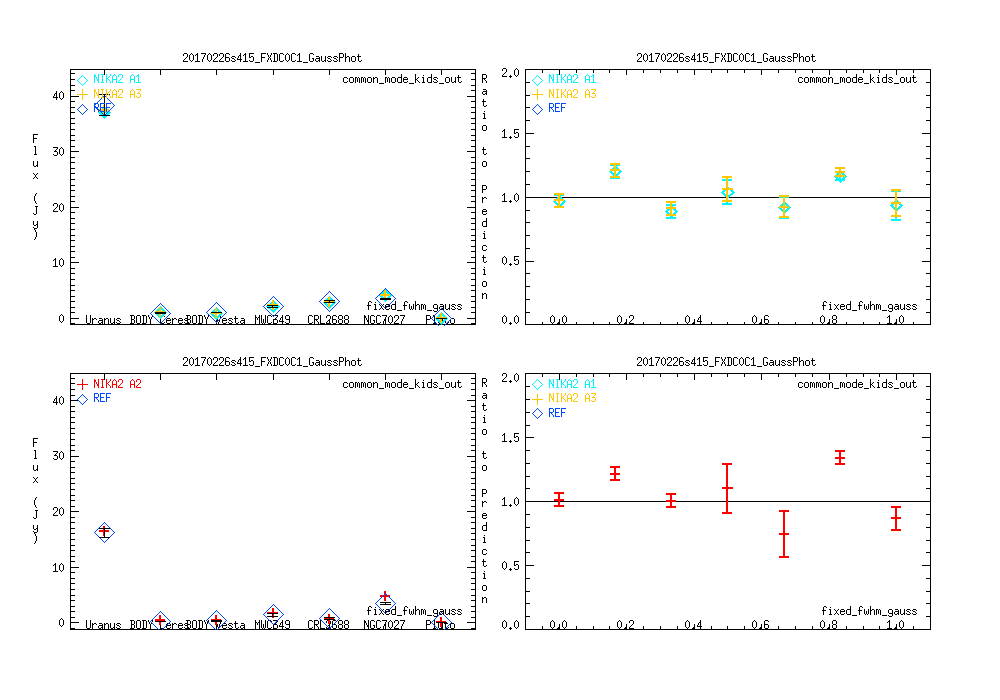
\includegraphics[clip, angle=0, scale = 0.4]{Figures/Calibrators_N2R9_20170226s415_FXDC0C1_GaussPhotFluxType_fixed_fwhm_gauss.png}
\caption{Decorrelation mask: 100 or 60 arcsec, KID cross-calib with fixed fwhm
  (12.5 and 18.5), then absolute photometry with the same fixed fwhm. Note:
  NGC7027 not point like and not corrected for here. Error bars from NIKA2
  measurements and abs. cal. uncertainties by JFL.}
\label{fig:fov}
\end{center}
\end{figure}


\subsection{Calibration stability across the run}

\begin{figure}
\begin{center}
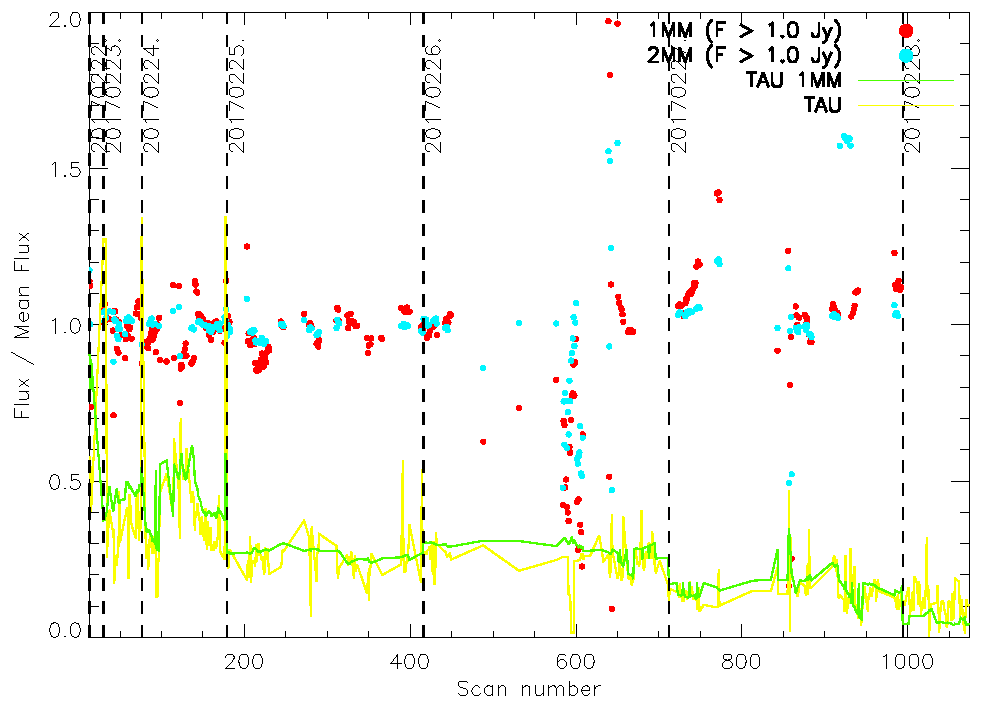
\includegraphics[clip, angle=0, scale = 0.7]{Figures/FluxIndScans/flux_ratio_run22.pdf}
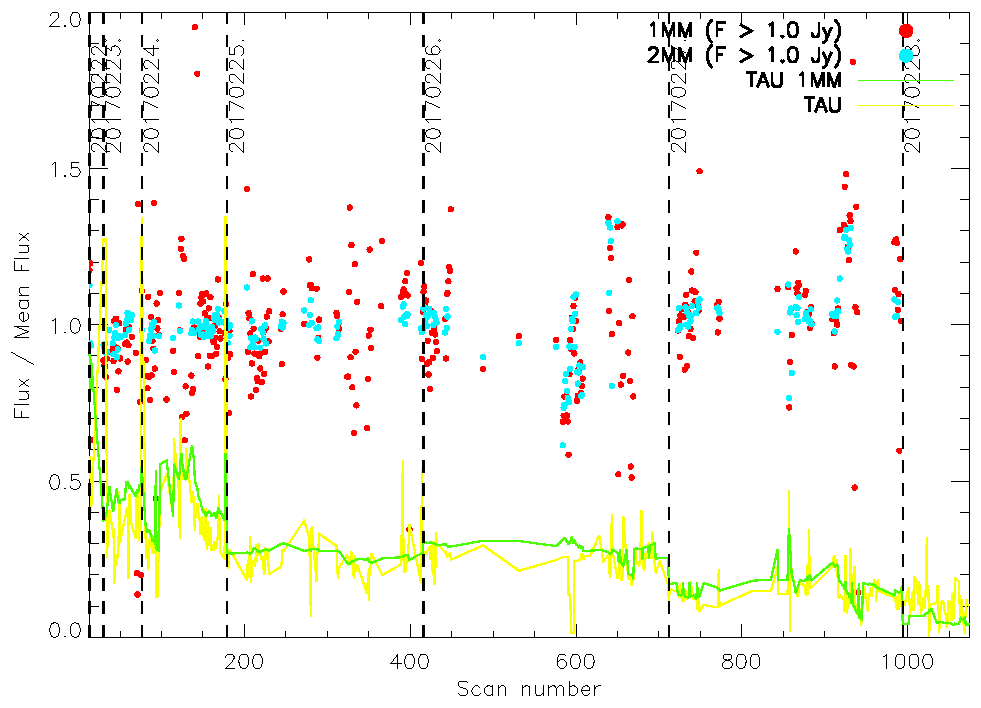
\includegraphics[clip, angle=0, scale = 0.7]{Figures/FluxIndScans/flux_ap_ratio_run22.pdf}
\caption{Ratio between the measured flux per scan and the averaged flux for all sources observed in N2R9. We considered both fixed FWHM (top) and aperture photometry fluxes for the 1 (red) and 2 (cyan) mm channels. }
\label{fig:fluxvsscan}
\end{center}
\end{figure}

\begin{figure}
\begin{center}
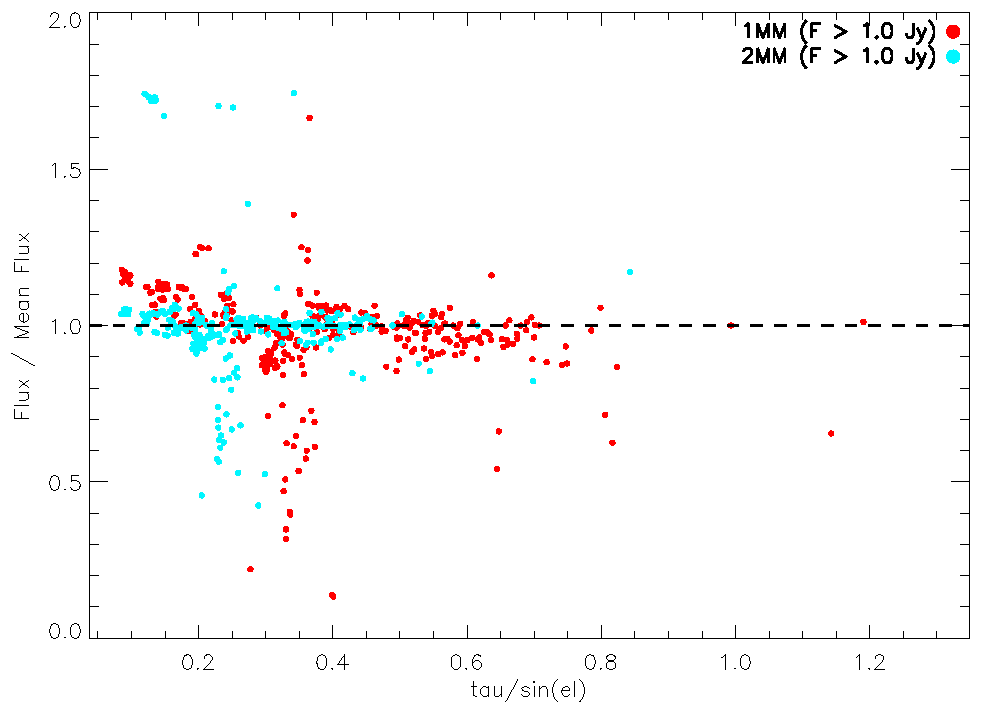
\includegraphics[clip, angle=0, scale = 0.7]{Figures/FluxIndScans/flux_ratio_rz_run22.pdf}
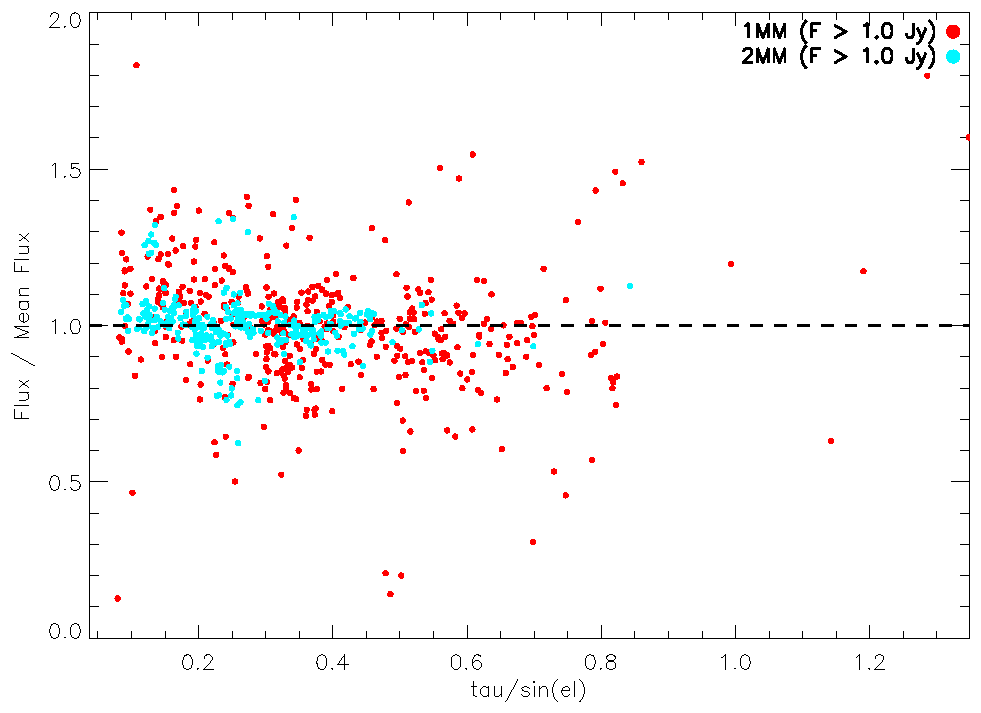
\includegraphics[clip, angle=0, scale = 0.7]{Figures/FluxIndScans/flux_ap_ratio_rz_run22.pdf}
\caption{Ratio between the measured flux per scan and the averaged flux as a function atmospheric backgroud for all sources observed in N2R9. We considered both fixed FWHM (top) and aperture photometry fluxes for the 1 (red) and 2 (cyan) mm channels. }
\label{fig:fluxvsbackground}
\end{center}
\end{figure}



%----------------------------------------------------------------------------------------
%	NOISE DESCRIPTION
%----------------------------------------------------------------------------------------
\section{Noise description: TOI and maps}
\label{se:noise}

\subsection{Dark detectors at 1 mm}
%\begin{figure}
%\begin{center}
%\includegraphics[clip, angle=0, scale = 0.7]{Figures/}
%\includegraphics[clip, angle=0, scale = 0.7]{Figures/FluxIndScans/}
%\caption{ Other stuff}
%\label{fig:fluxvsbackground}
%\end{center}
%\end{figure}


%----------------------------------------------------------------------------------------
%	DARK TESTS
%----------------------------------------------------------------------------------------
\subsection{Dark tests}
\label{se:dark}
\section{Detector-Detector correlation matrix}

For this work we have used several decorrelation methods trying to identify possible multiple components in the noise. Notice that in the following the atmospheric signal will be considered simply as correlated sky noise. The main decorrelation methods used are:

\begin{enumerate}
\item[CM] {\bf Common mode decorrelation}. We search for a common mode template using all detectors of the same array. To avoid bias from bad detectors we consider the median common mode.

\item[PCA] {\bf Principal Component Analysis}. For each NIKA2 array independently we decompose the covariance matrix in principal components. From those we derive up to 10 independent templates corresponding to the largest eigenvalue values.

\item[BC] {\bf Best correlated pixels}. For each detector in a given array we identify those detectors which are more correlated to it (a minimum of 14). Using those detectors we compute a common mode as in method CM. 

\item[ALL] {\bf All detectors}. For earch detector of a given array we use all other detectors of the same array as templates and perform a linear fit.

\end{enumerate}

We present in Figure~\ref{corrs299} the detector noise correlation matrices computed for the N2R7 dark scan 20161211s299 for the three arrays (A1, A2, and A3 from left to right). From top to bottom we present the correlation matrices for the raw data (no decorrelation), and for the CM, PCA, and BC decorrelated data. For each array the extent and name (from letter A to T) of the electronic boxes is indicated on the left of the figure. Notice that each electronic box consists of 5 subbands. \\

In the case of the raw data we observe very different structures for the three arrays. In arrays A1 and A2, we observe significant structure going from very correlated detectors to fully uncorrelated ones. This is observed even within a given electronic box or even between detectors from the same electronic subband. By contrast in A3 the detectors seems to be fully correlated. After CM decorrelation we observe that there is still significant correlation and anti-correlation for some detectors. In particular we observe a very clear pattern in A2 for electronic box A. In the case of the PCA decorrelated data the correlation matrix becomes much more diagonal although still shows significant level correlation within electronic subbands. We also notice that using the BC decorrelation improves with respect to the CM decorrelation but it is worse than the PCA case. These results tends indicate various electronic or detector related noise components. \\

In Figure~\ref{corrs72} we show the noise correlation matrices for the N2R7 faint source scan 20161213s72. As expected the raw data noise correlation is dominated by atmospheric noise and we observe full correlation between detectors. After decorrelation the results are very similar to those found for N2R7 dark scan 20161211s299. There is residual significant correlation and anti-correlation after CM decorrelation. PCA decorrelation leads to a more diagonal correlation matrices. For the BC decorrelation the results are worse (more residual correlation and anti-correlation) and close to those of the CM decorrelation. As before there are good indications of multiple electronic-detector noise components. It is interesting to note that the detector-electronic noise correlation patterns seems to be the same for dark tests and for sky data. 

We have repeated the same analysis on scans of the N2R4 both for dark tests, scan 20160504s97, and faint sources, scan 20160313s87. We find few significant differences with respect to previoius results. In the case of the dark test and for the raw data, the A1 and A2 detectors seems to be more correlated. Furthermore A2 show more significant correlation after CM decorrelation for electronic boxes B and D. Array A1 show also significant residual correlation and anti-correlation after CM et BC decorrelations. For the faint source N2R4 scan 
20160313s87 we observe similar behavior but the pattern of the correlation matrices are not the same that for the dark test scan.

\begin{figure}[ht] % Inline image example
\begin{center}
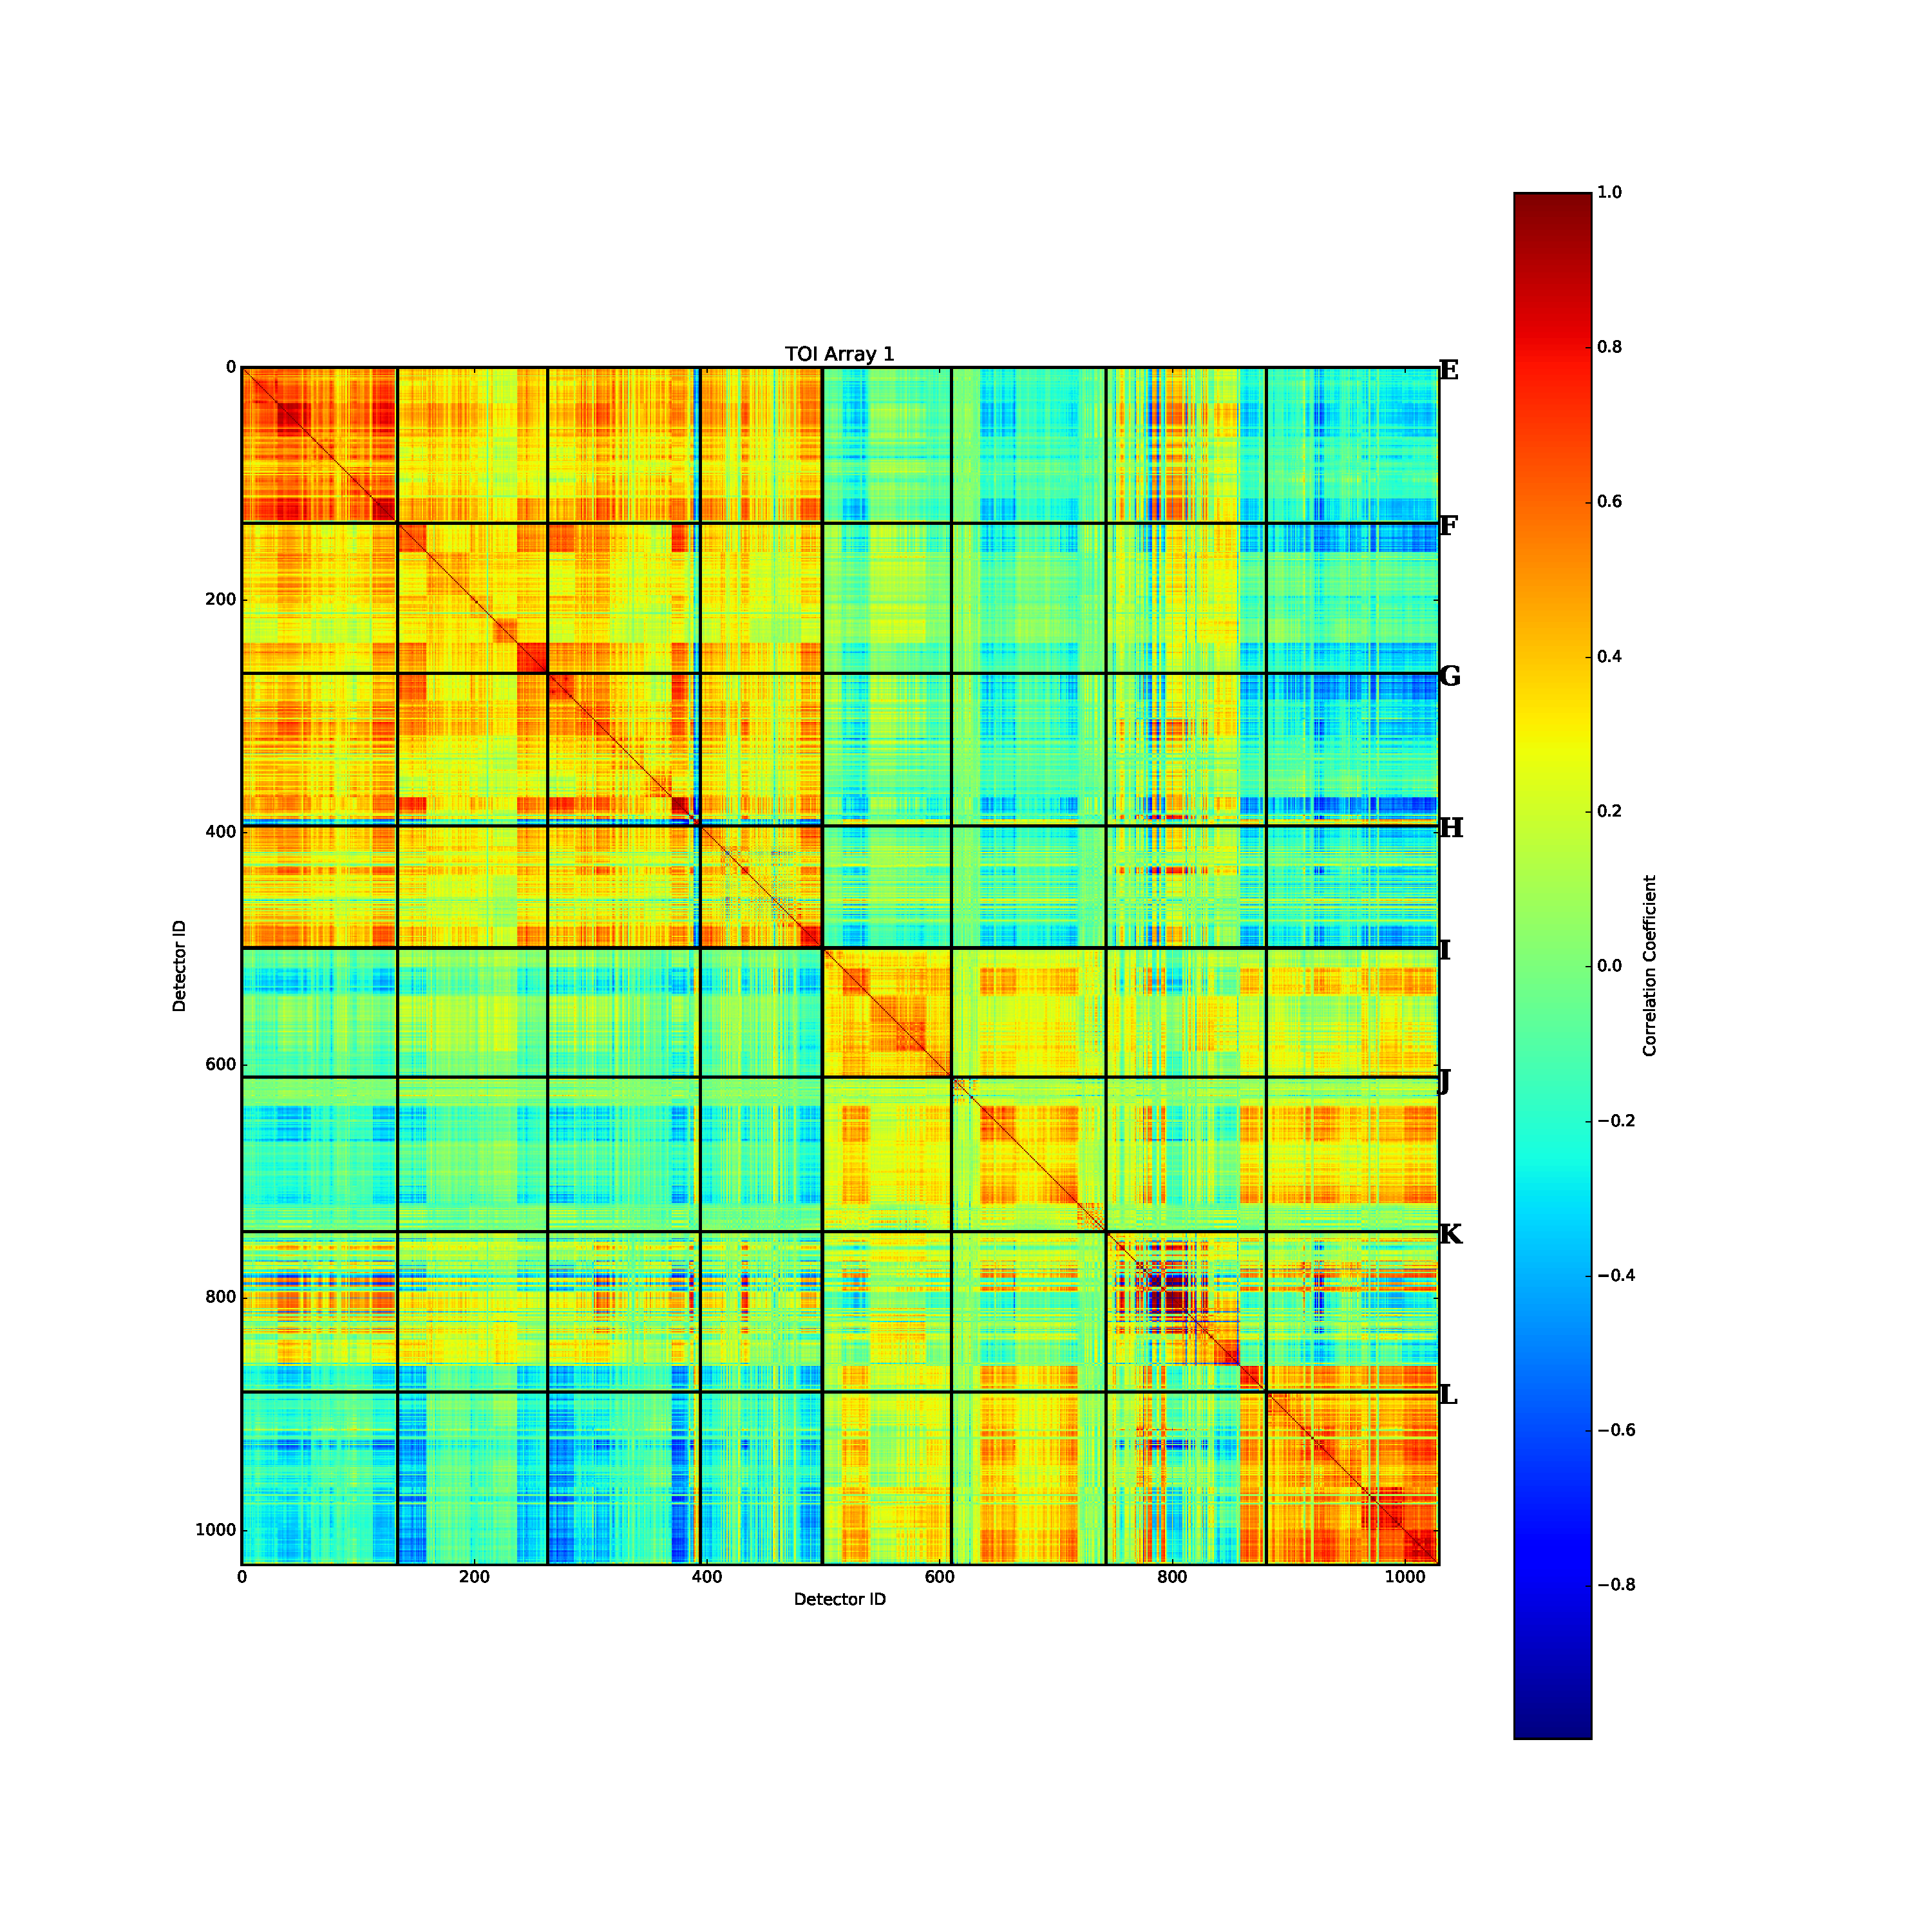
\includegraphics[width=0.3\textwidth]{Figures/DarkTests/corrmat_TOI_array_1_20161211s299.pdf}
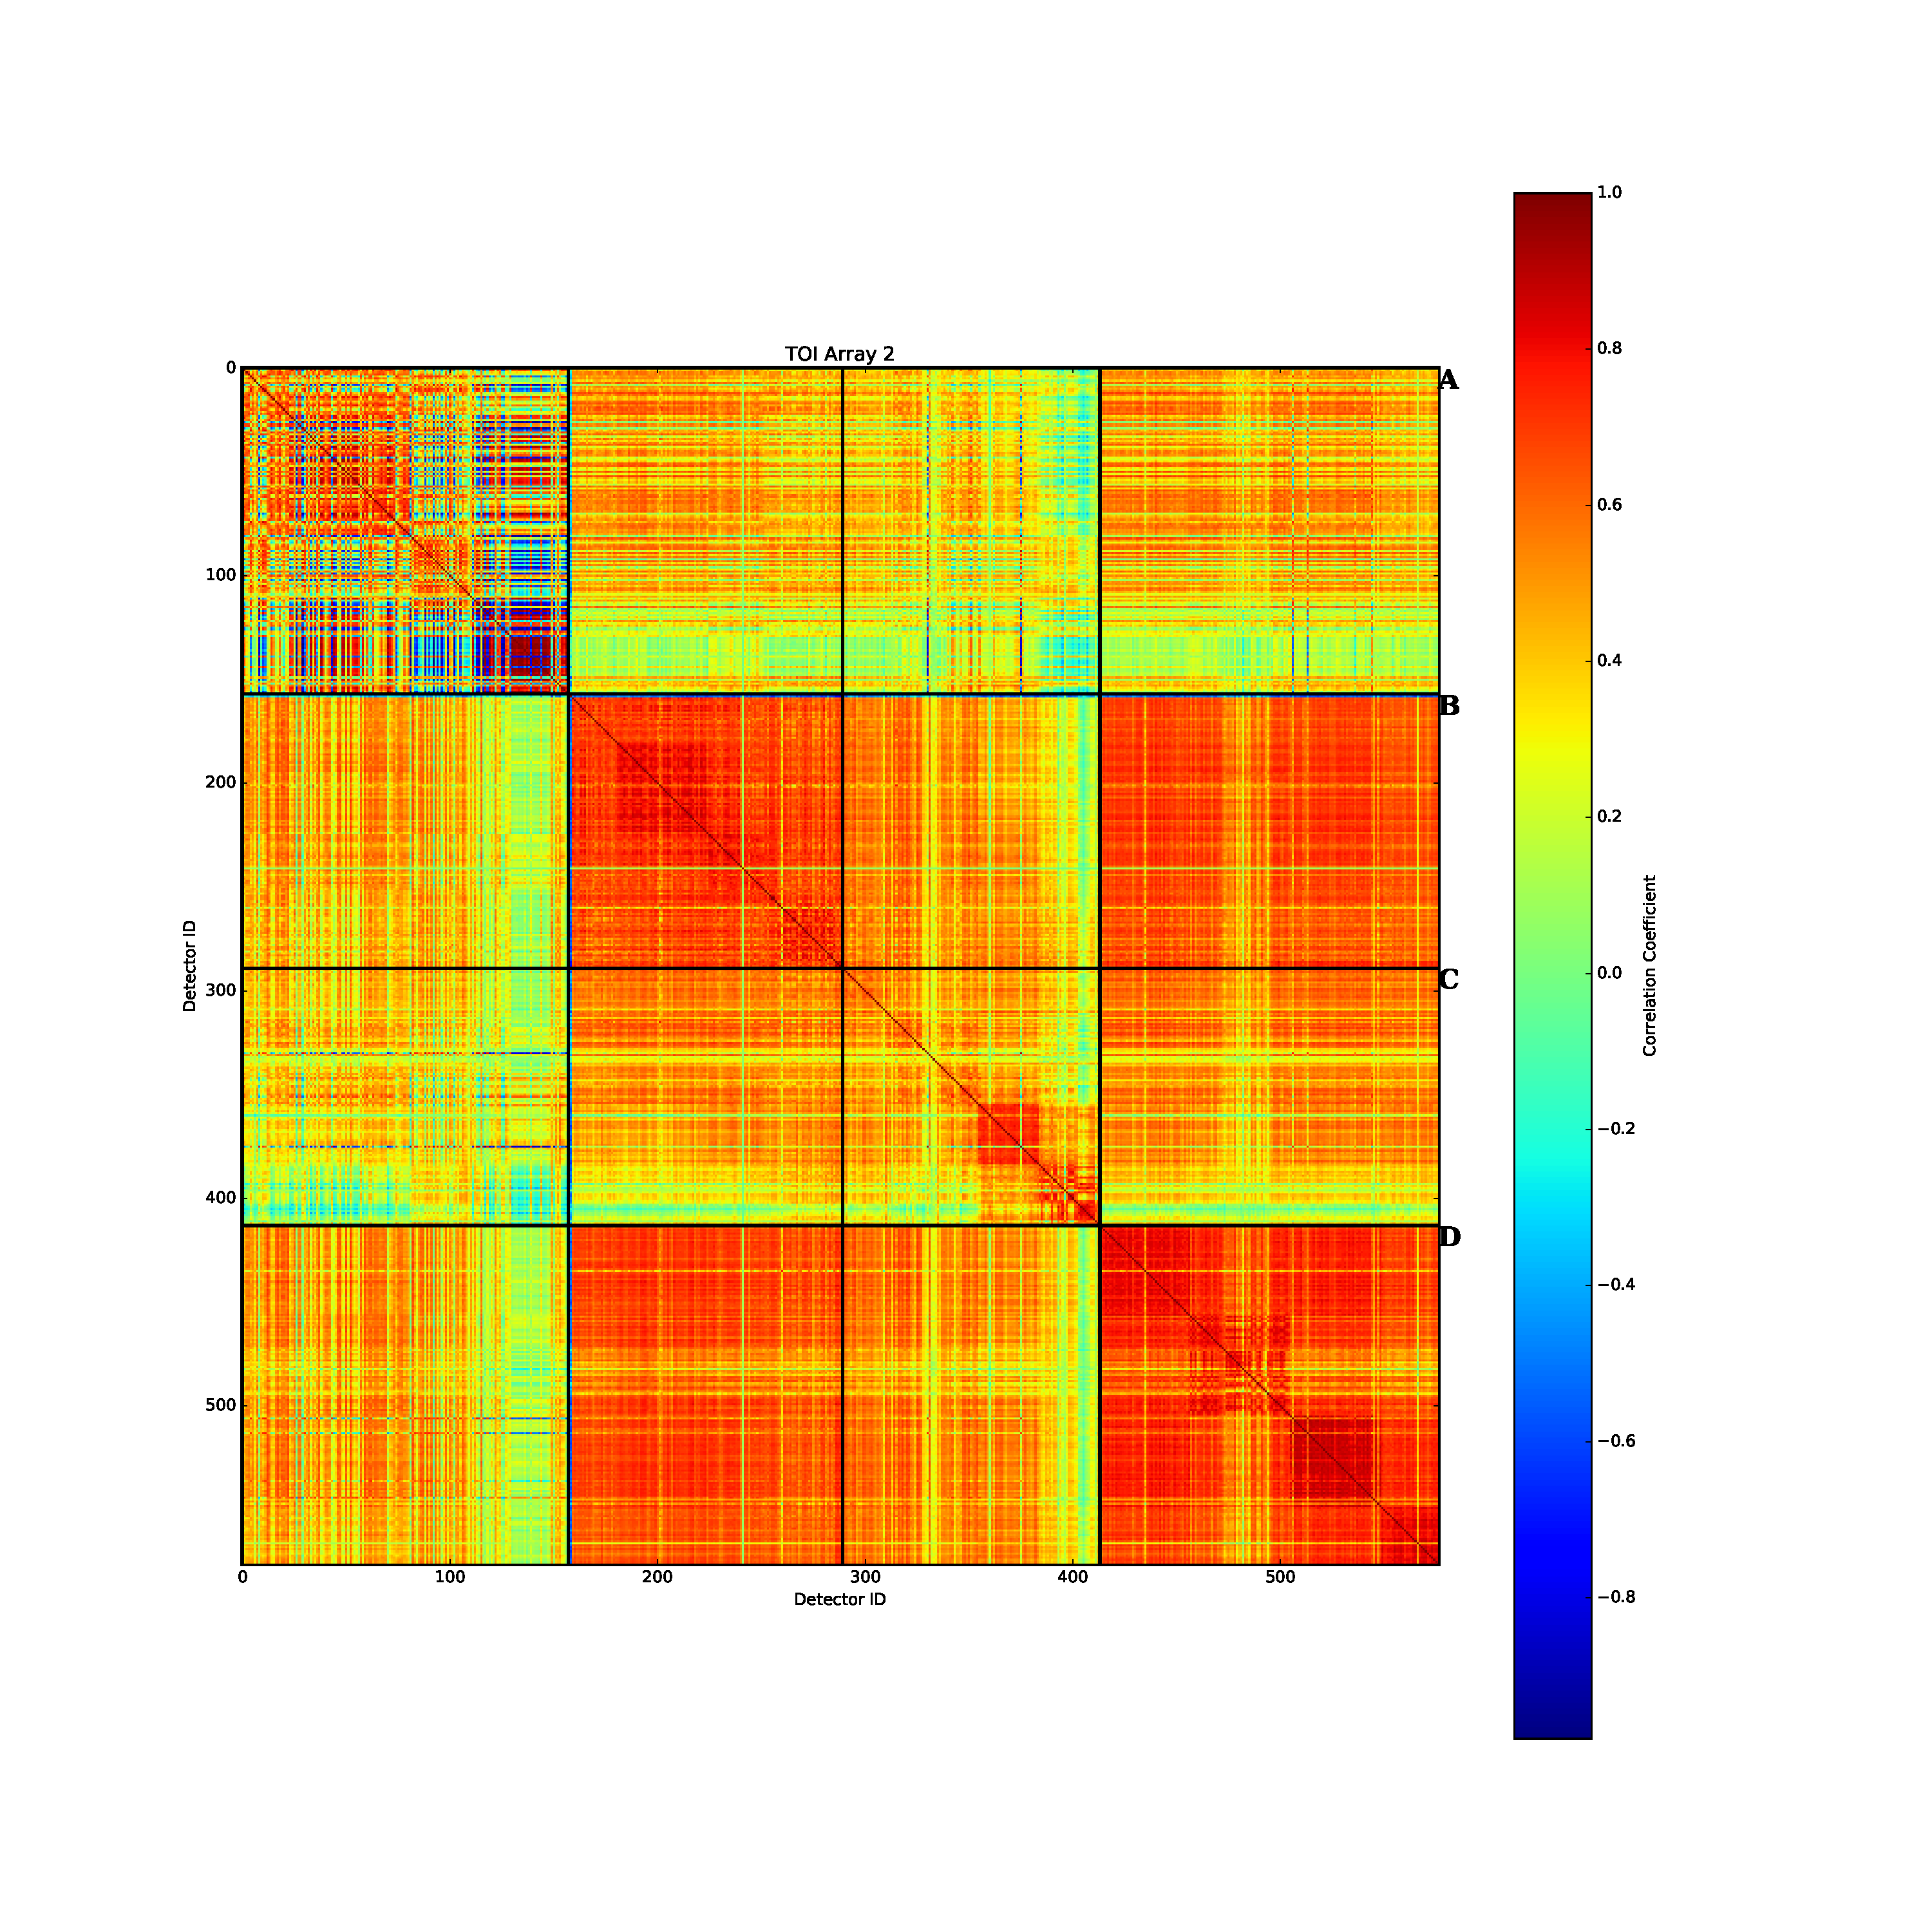
\includegraphics[width=0.3\textwidth]{Figures/DarkTests/corrmat_TOI_array_2_20161211s299.pdf}
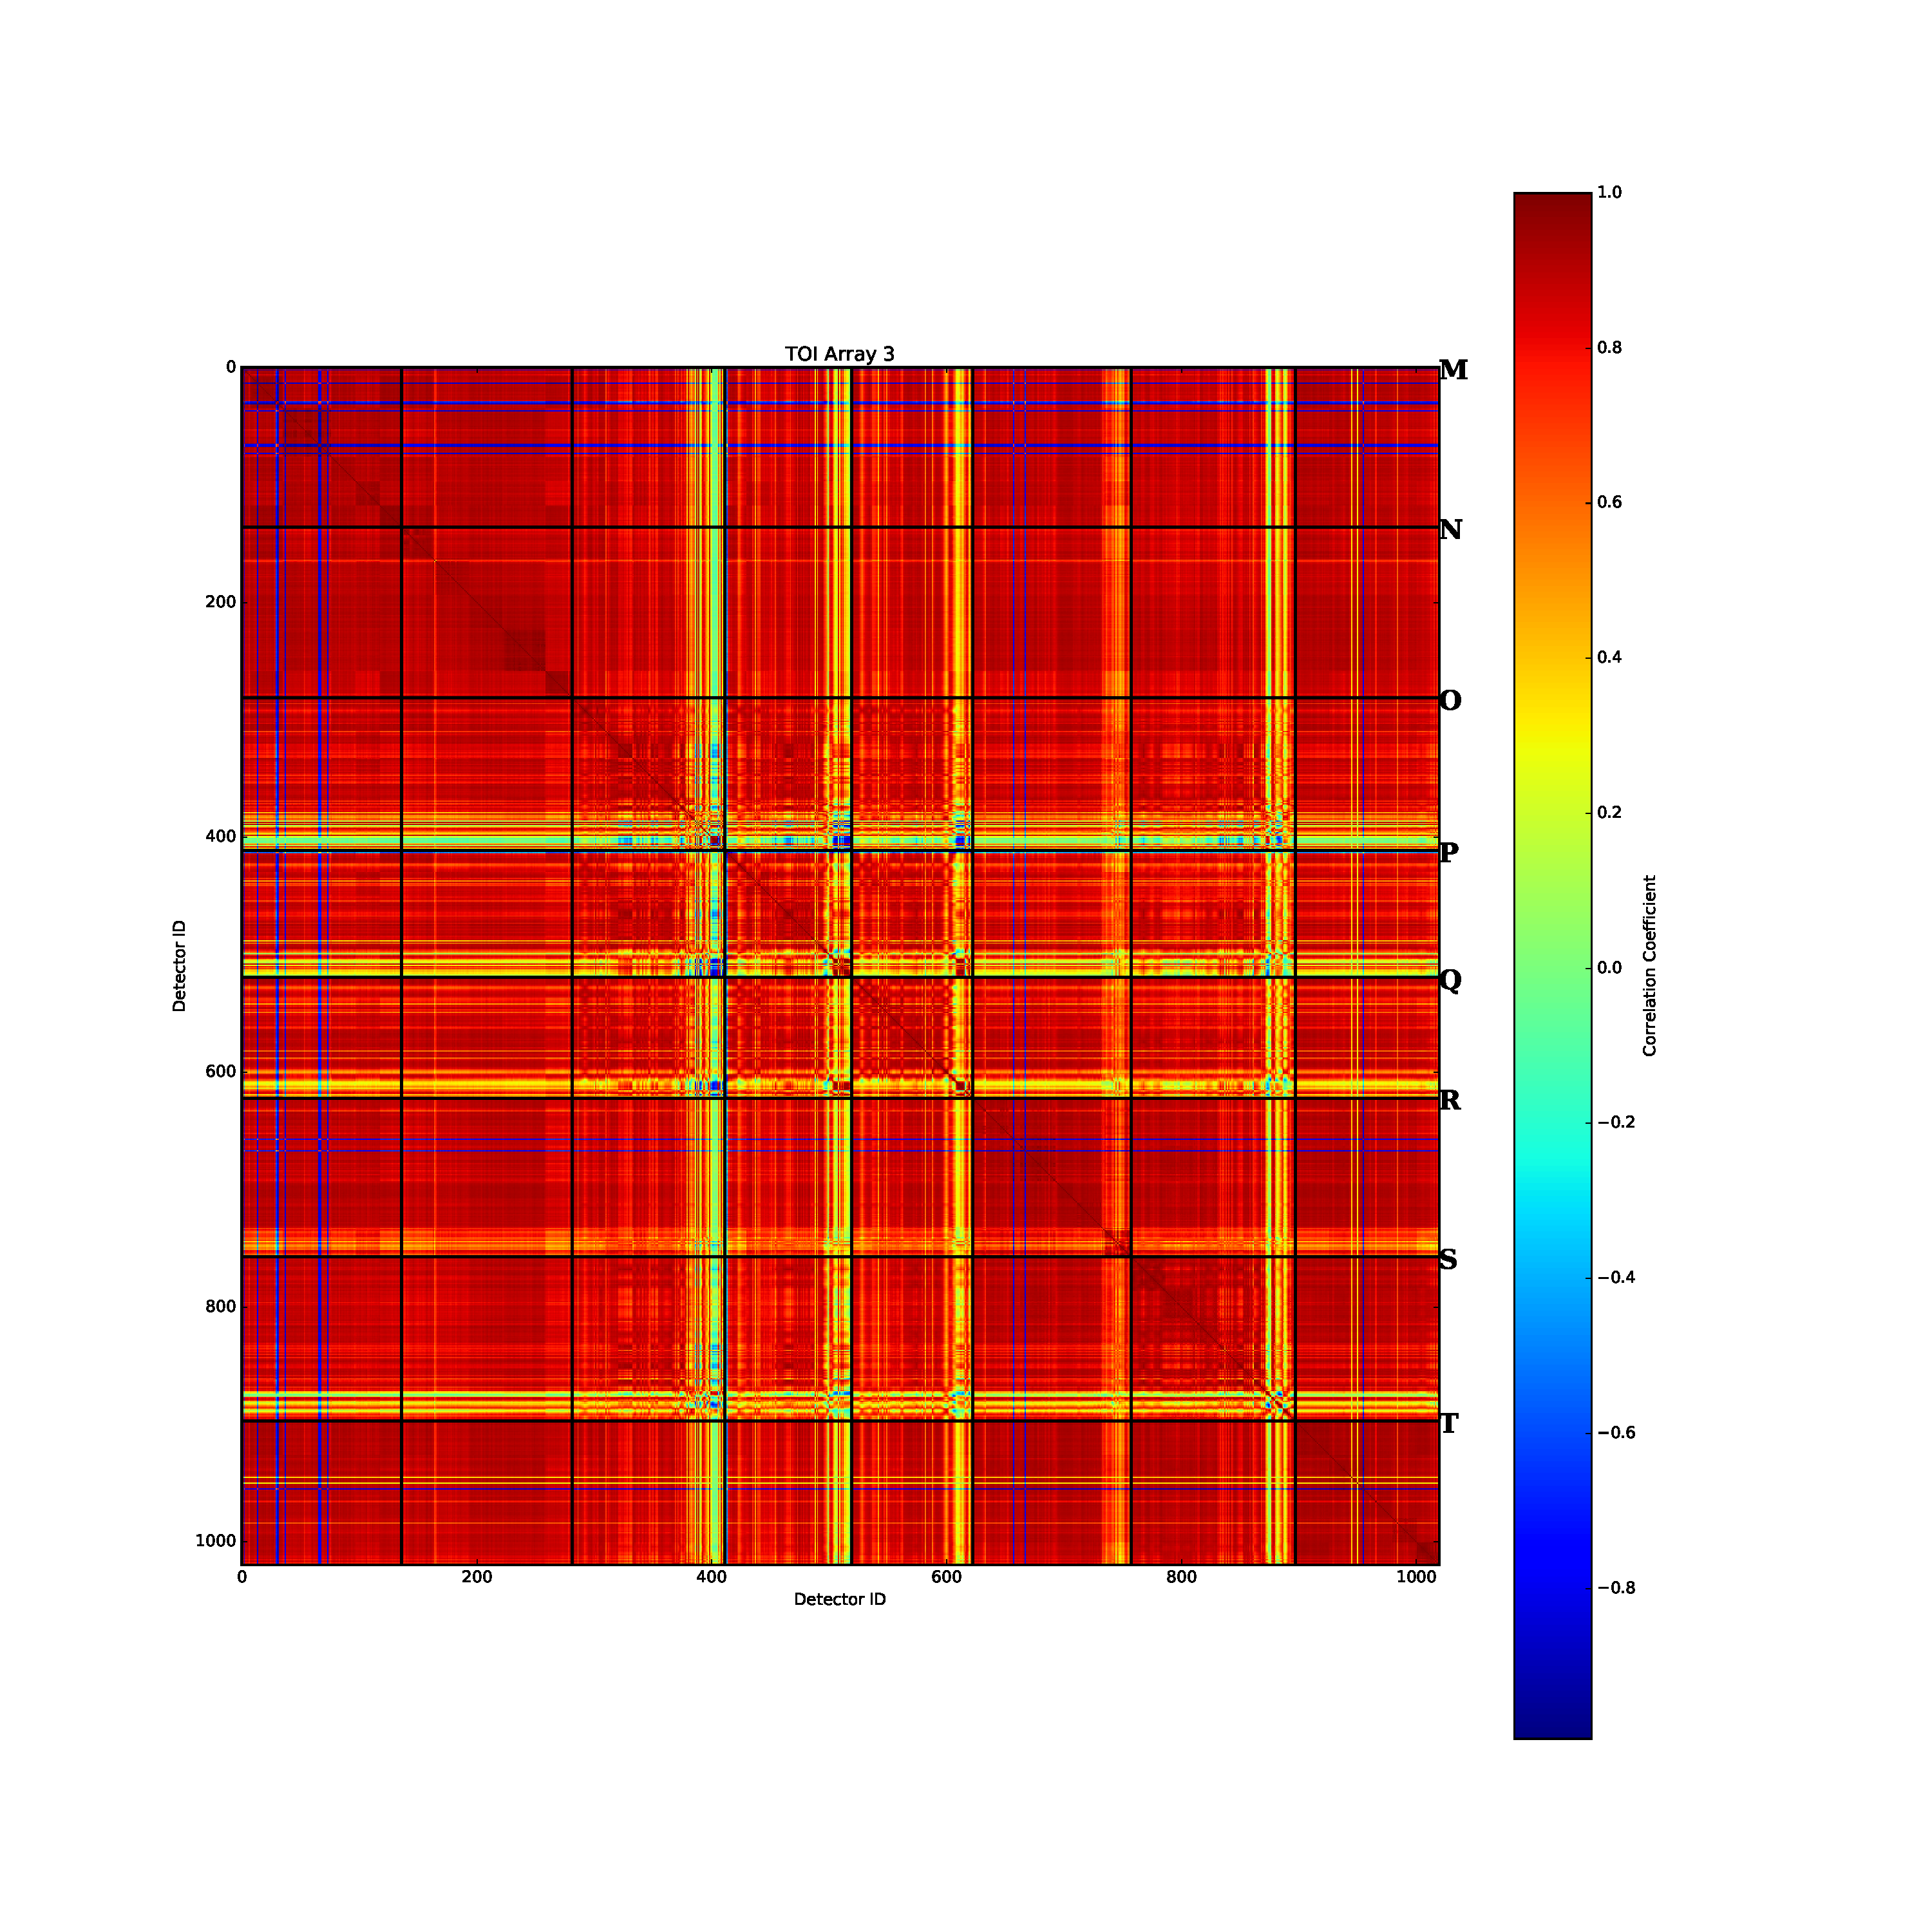
\includegraphics[width=0.3\textwidth]{Figures/DarkTests/corrmat_TOI_array_3_20161211s299.pdf}
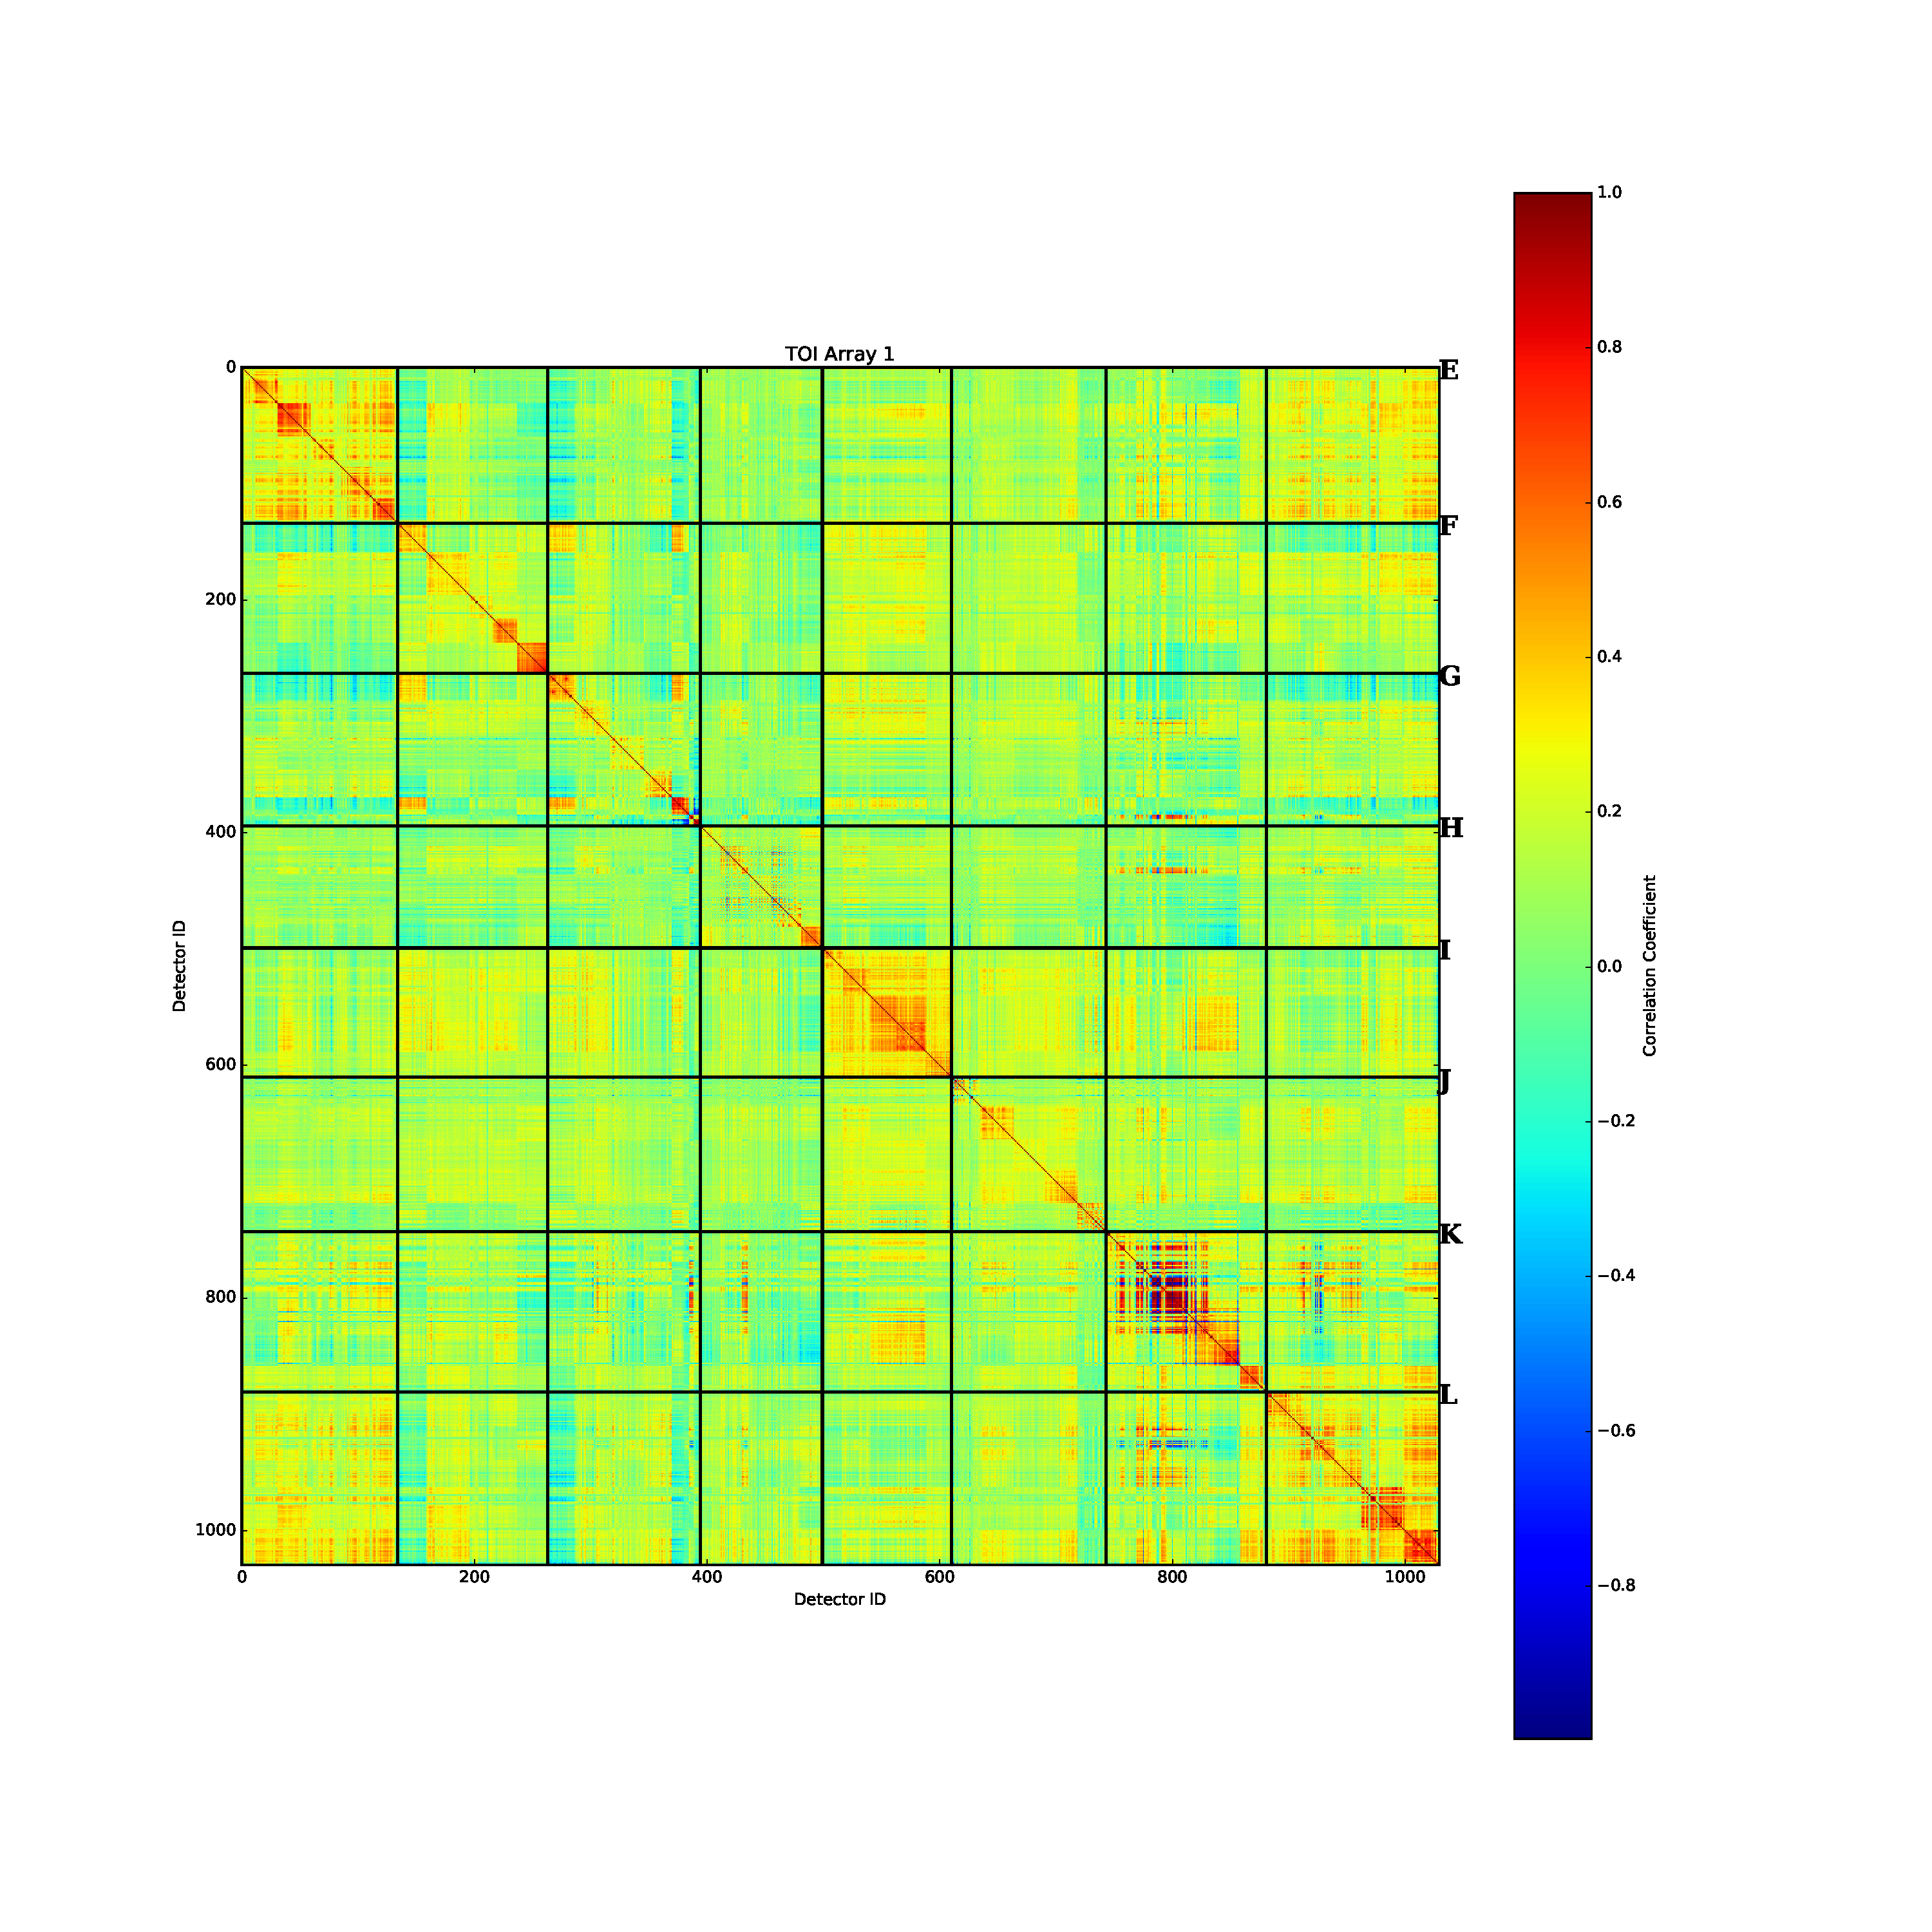
\includegraphics[width=0.3\textwidth]{Figures/DarkTests/corrmat_TOI_CM_array_1_20161211s299.pdf}
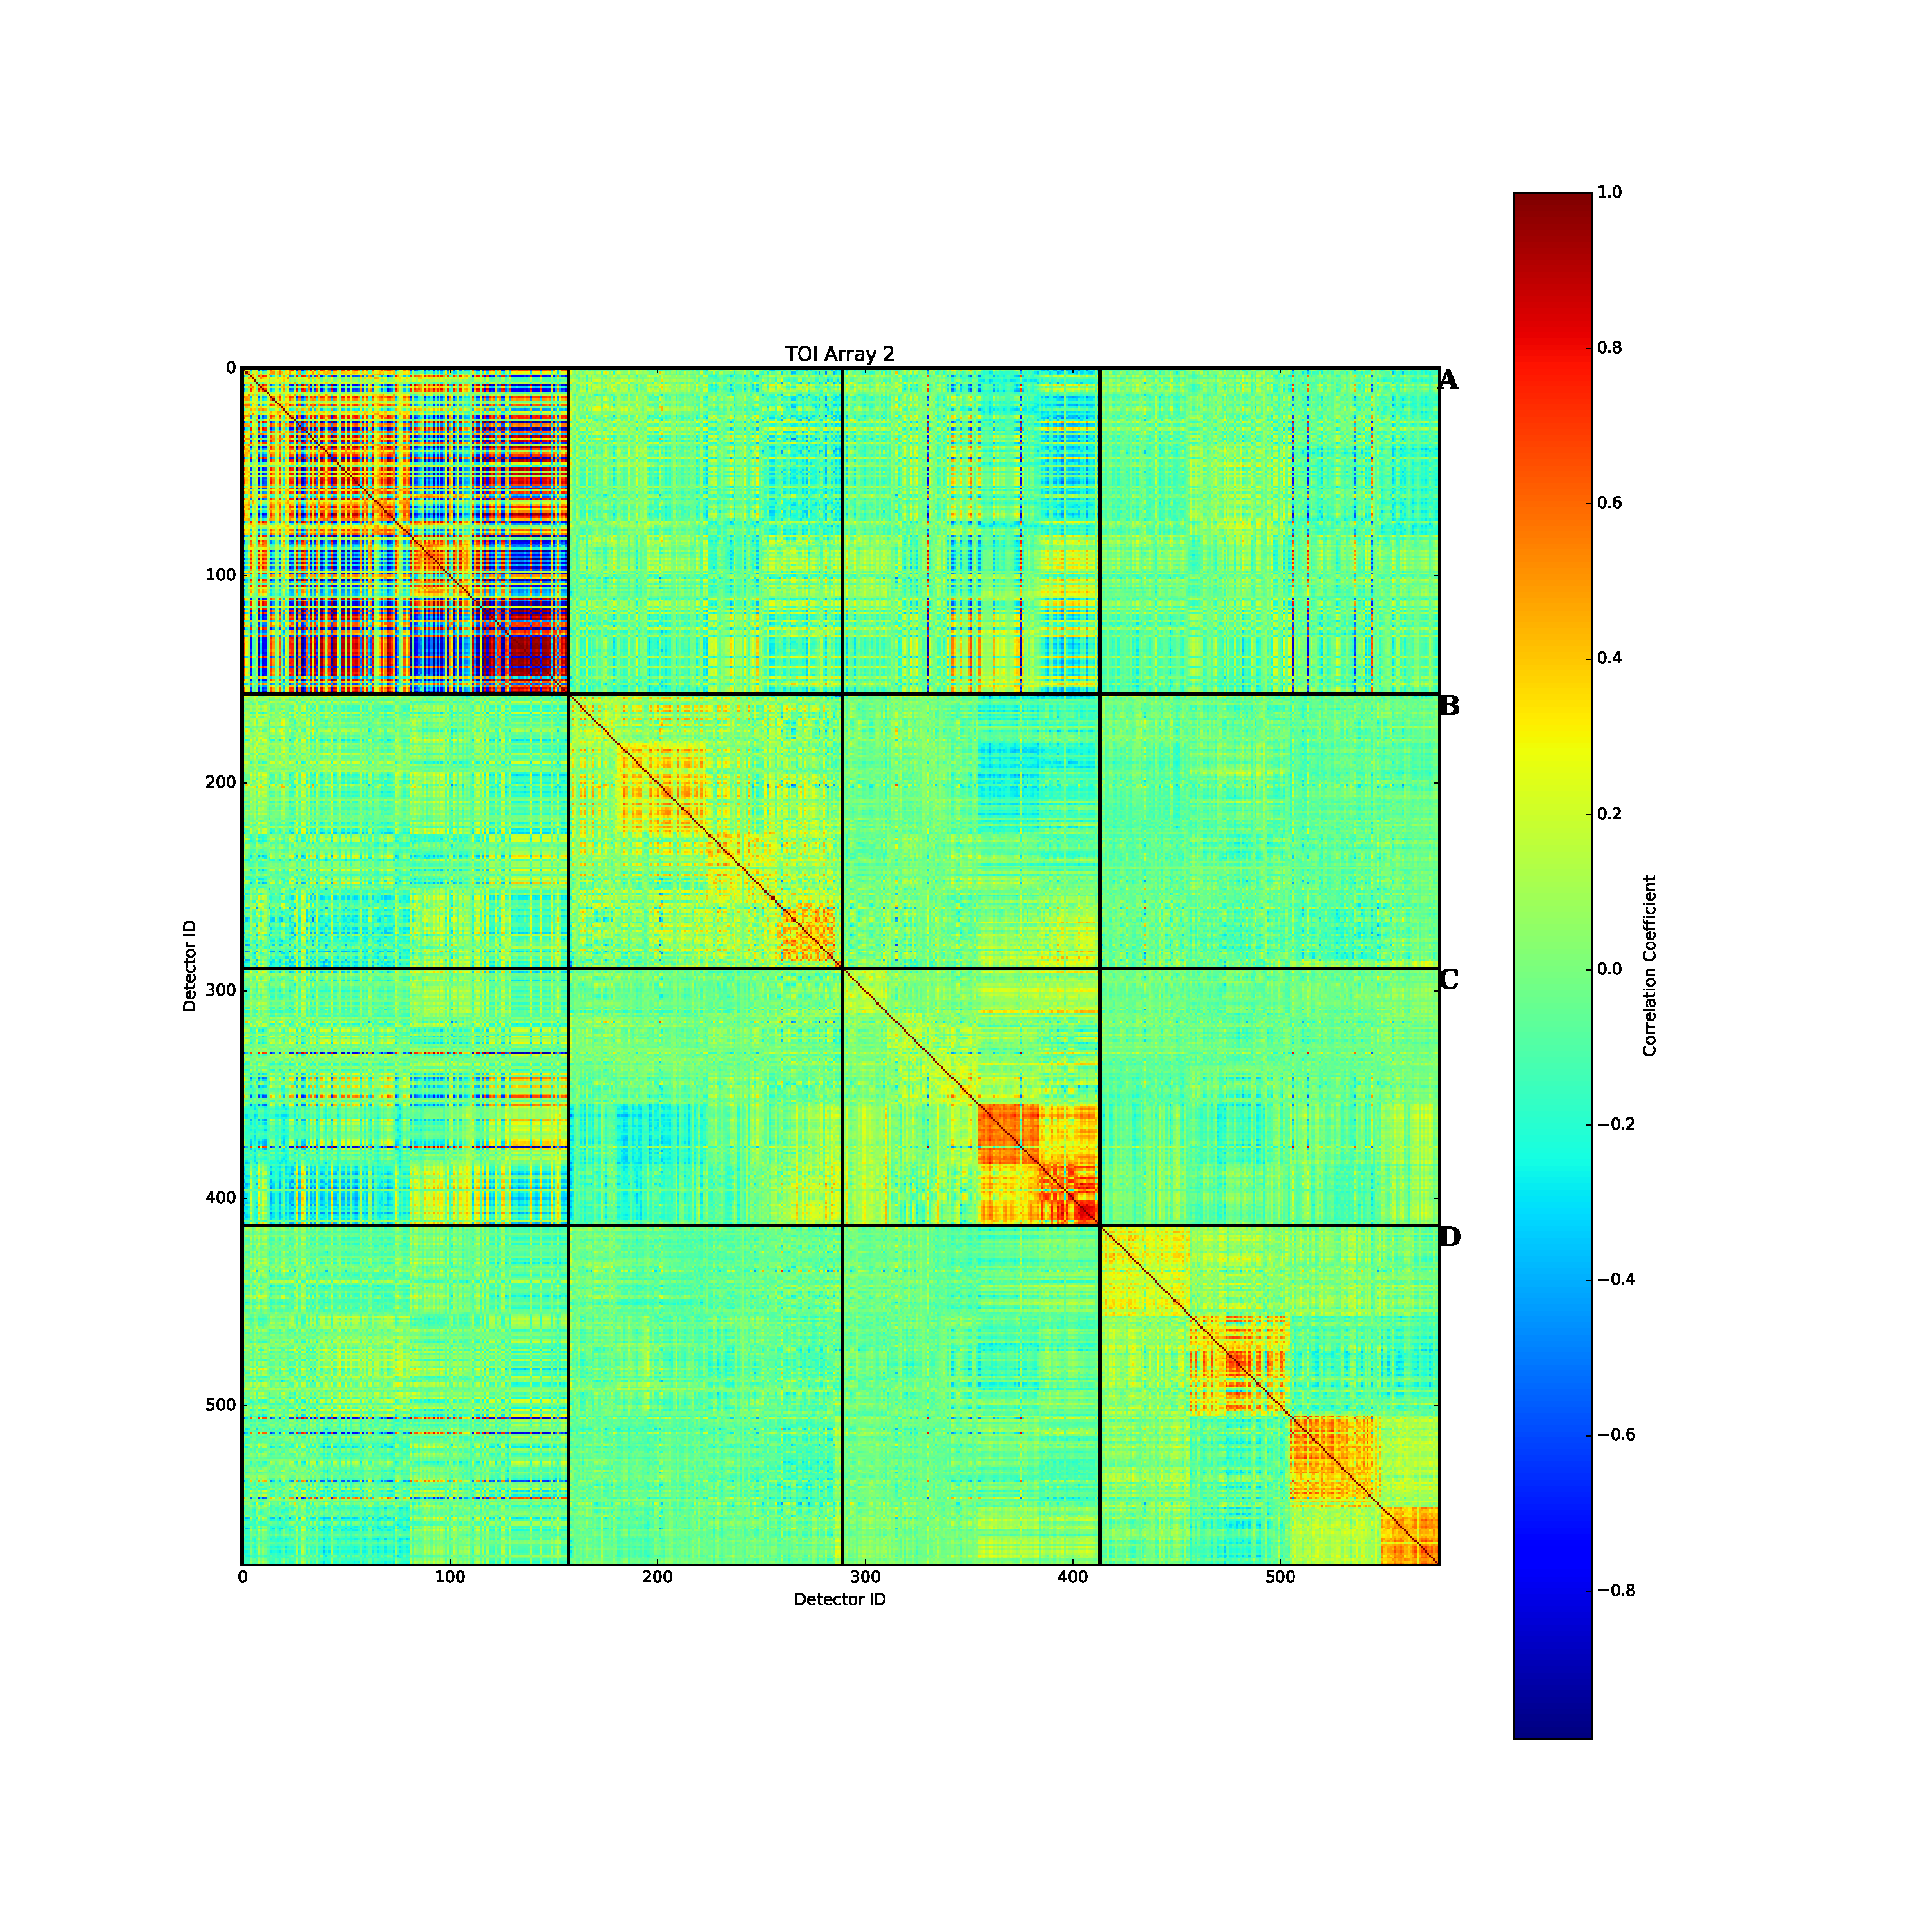
\includegraphics[width=0.3\textwidth]{Figures/DarkTests/corrmat_TOI_CM_array_2_20161211s299.pdf}
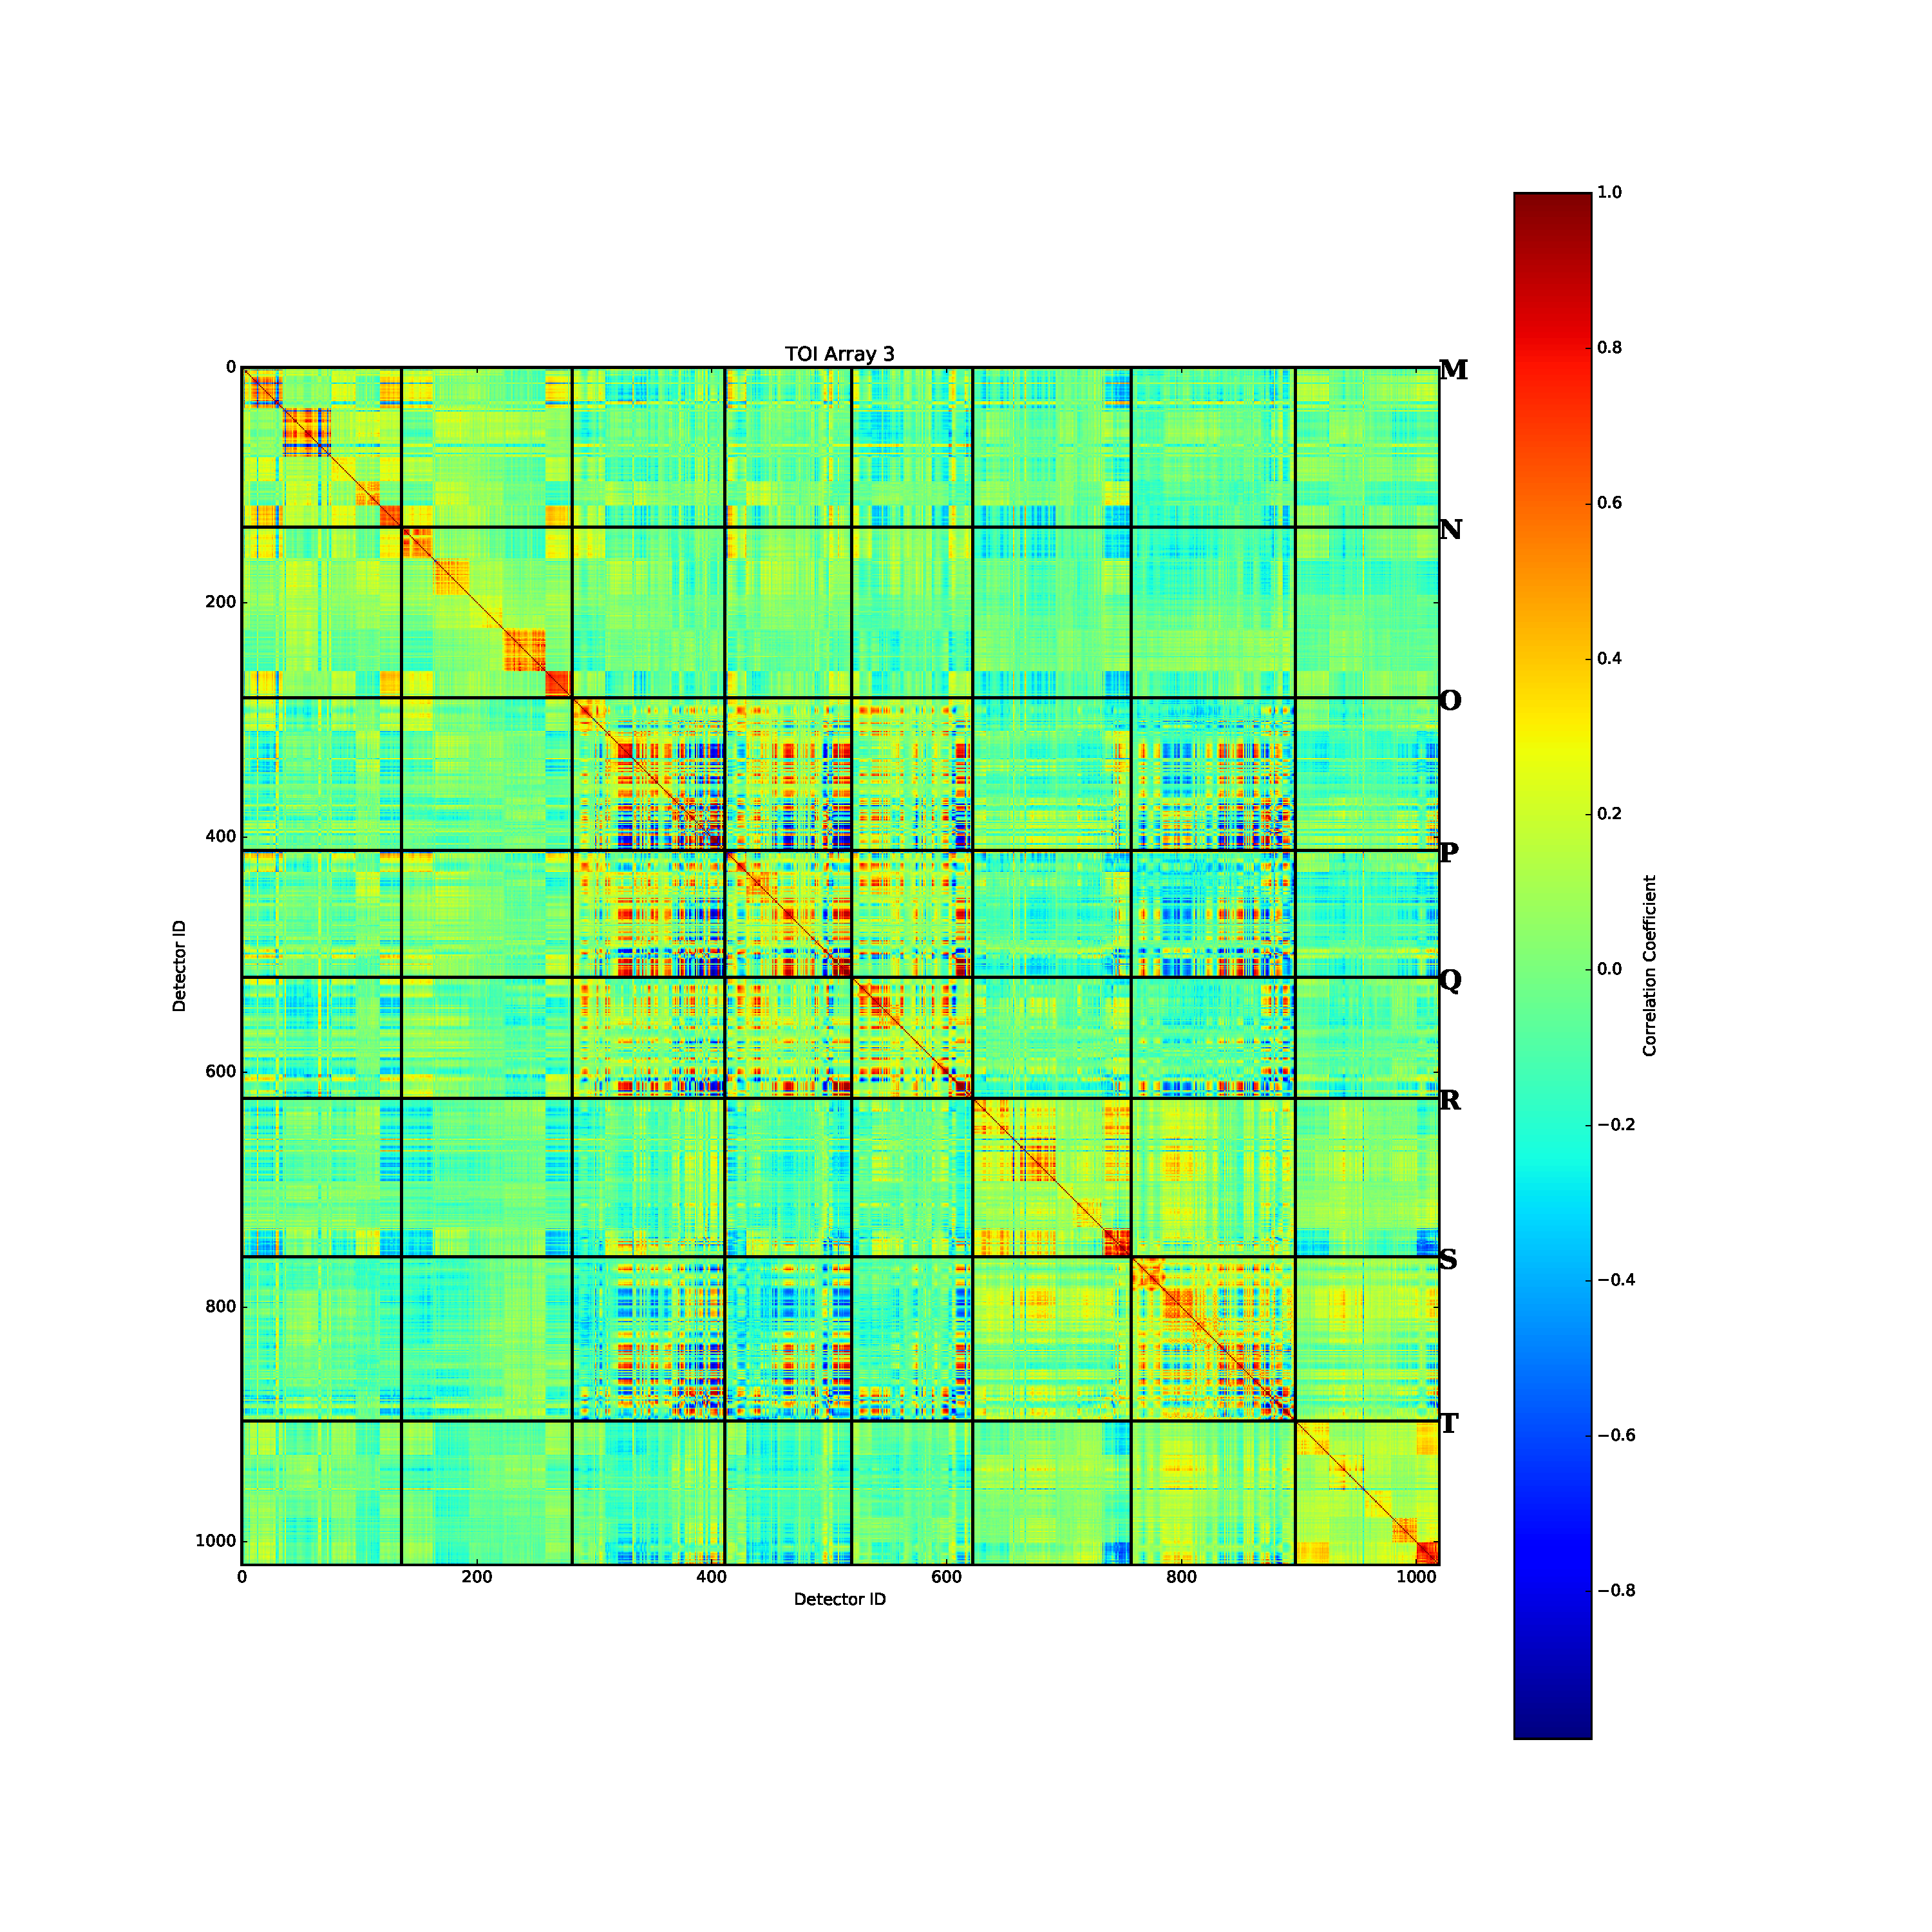
\includegraphics[width=0.3\textwidth]{Figures/DarkTests/corrmat_TOI_CM_array_3_20161211s299.pdf}
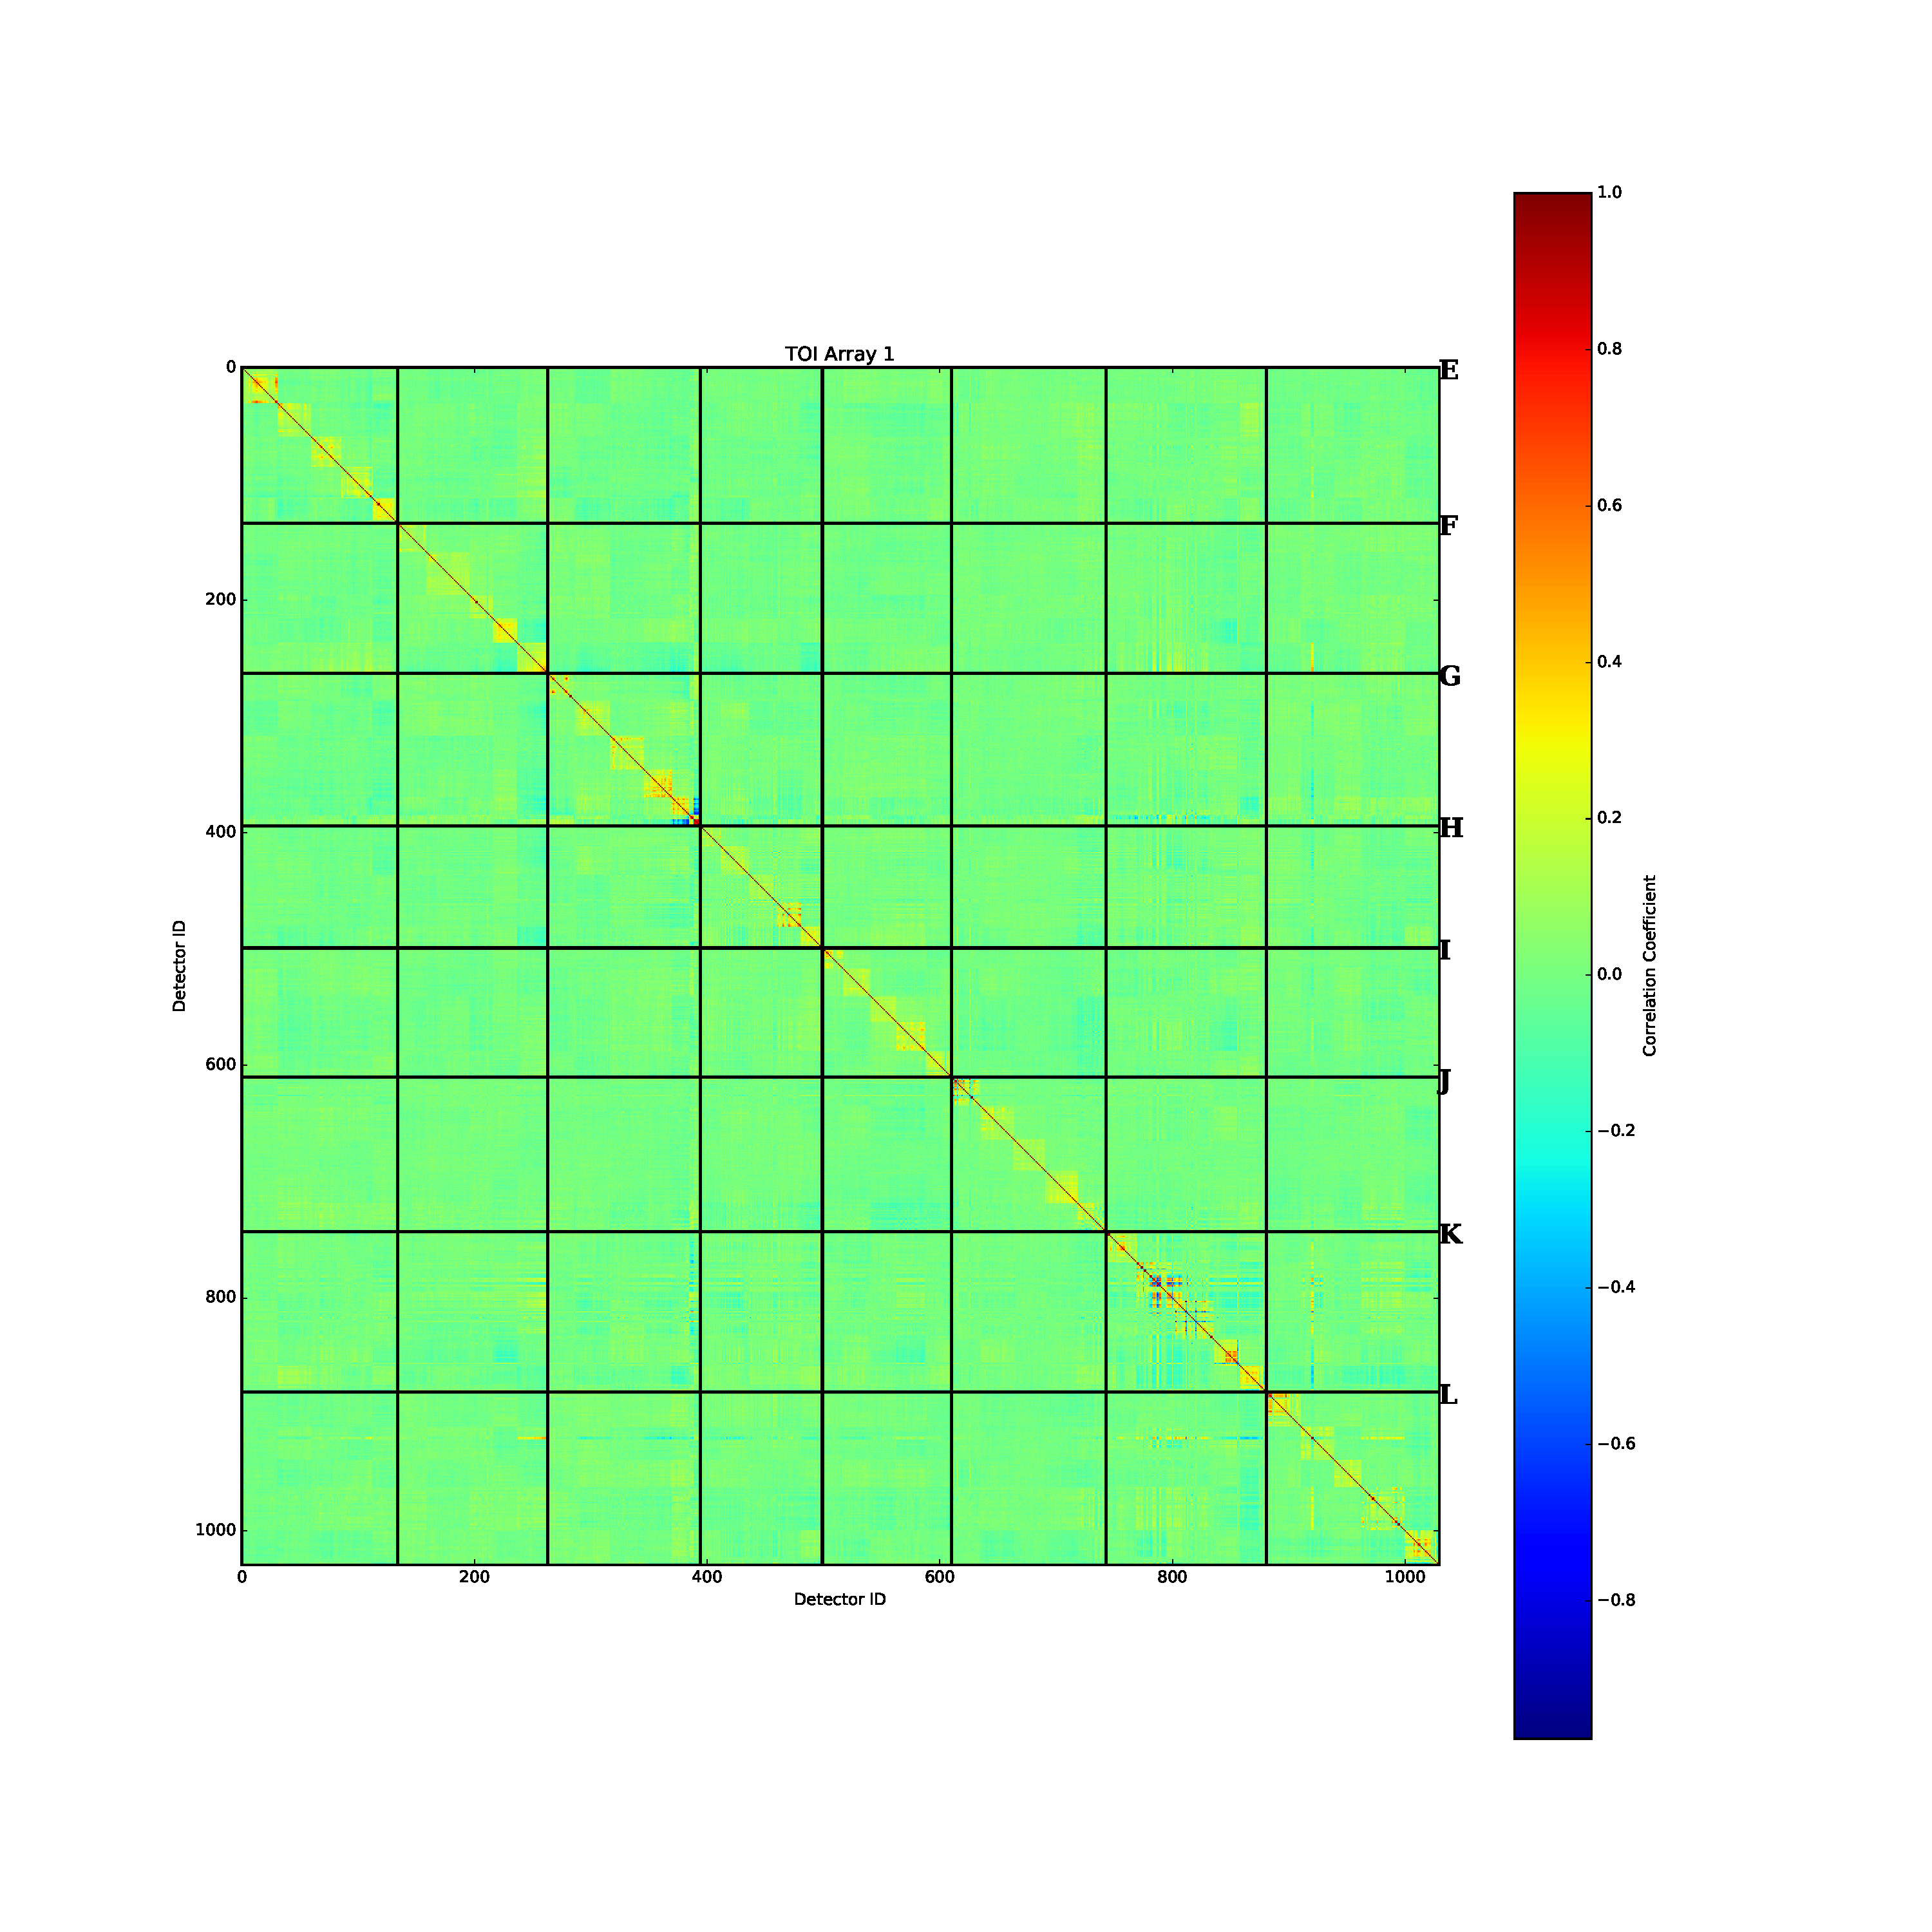
\includegraphics[width=0.3\textwidth]{Figures/DarkTests/corrmat_TOI_PCA_array_1_20161211s299.pdf}
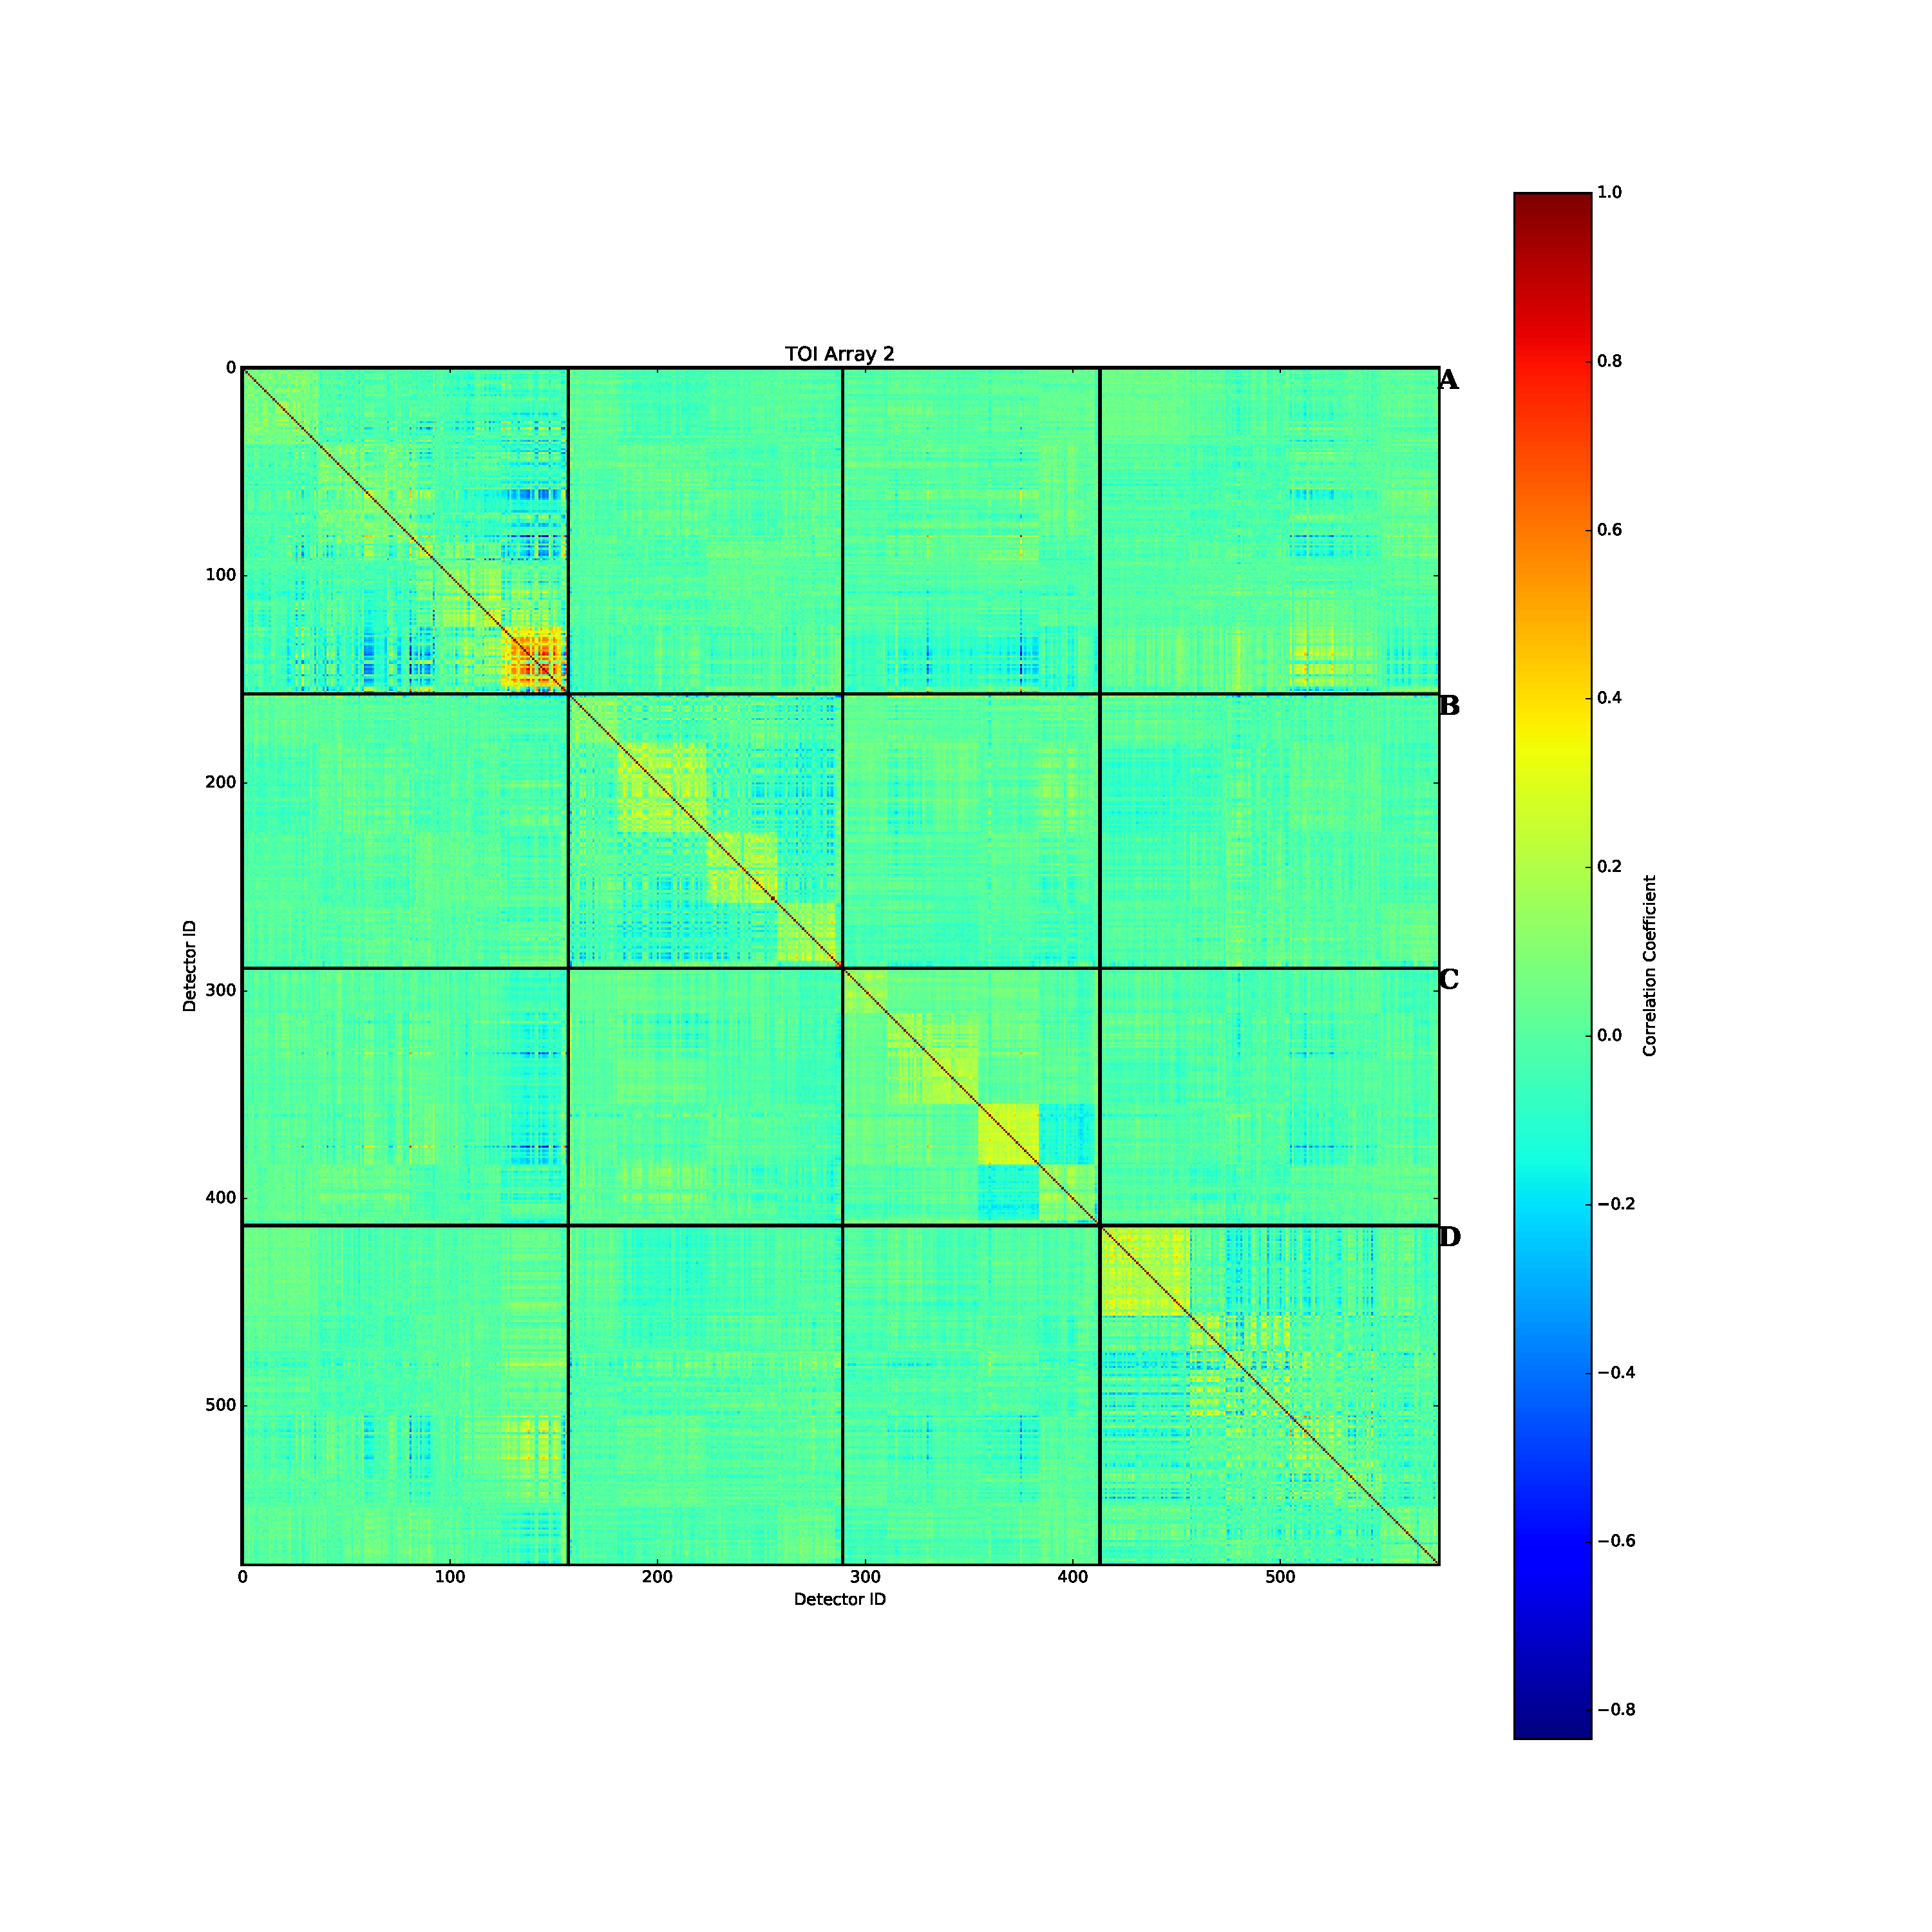
\includegraphics[width=0.3\textwidth]{Figures/DarkTests/corrmat_TOI_PCA_array_2_20161211s299.pdf}
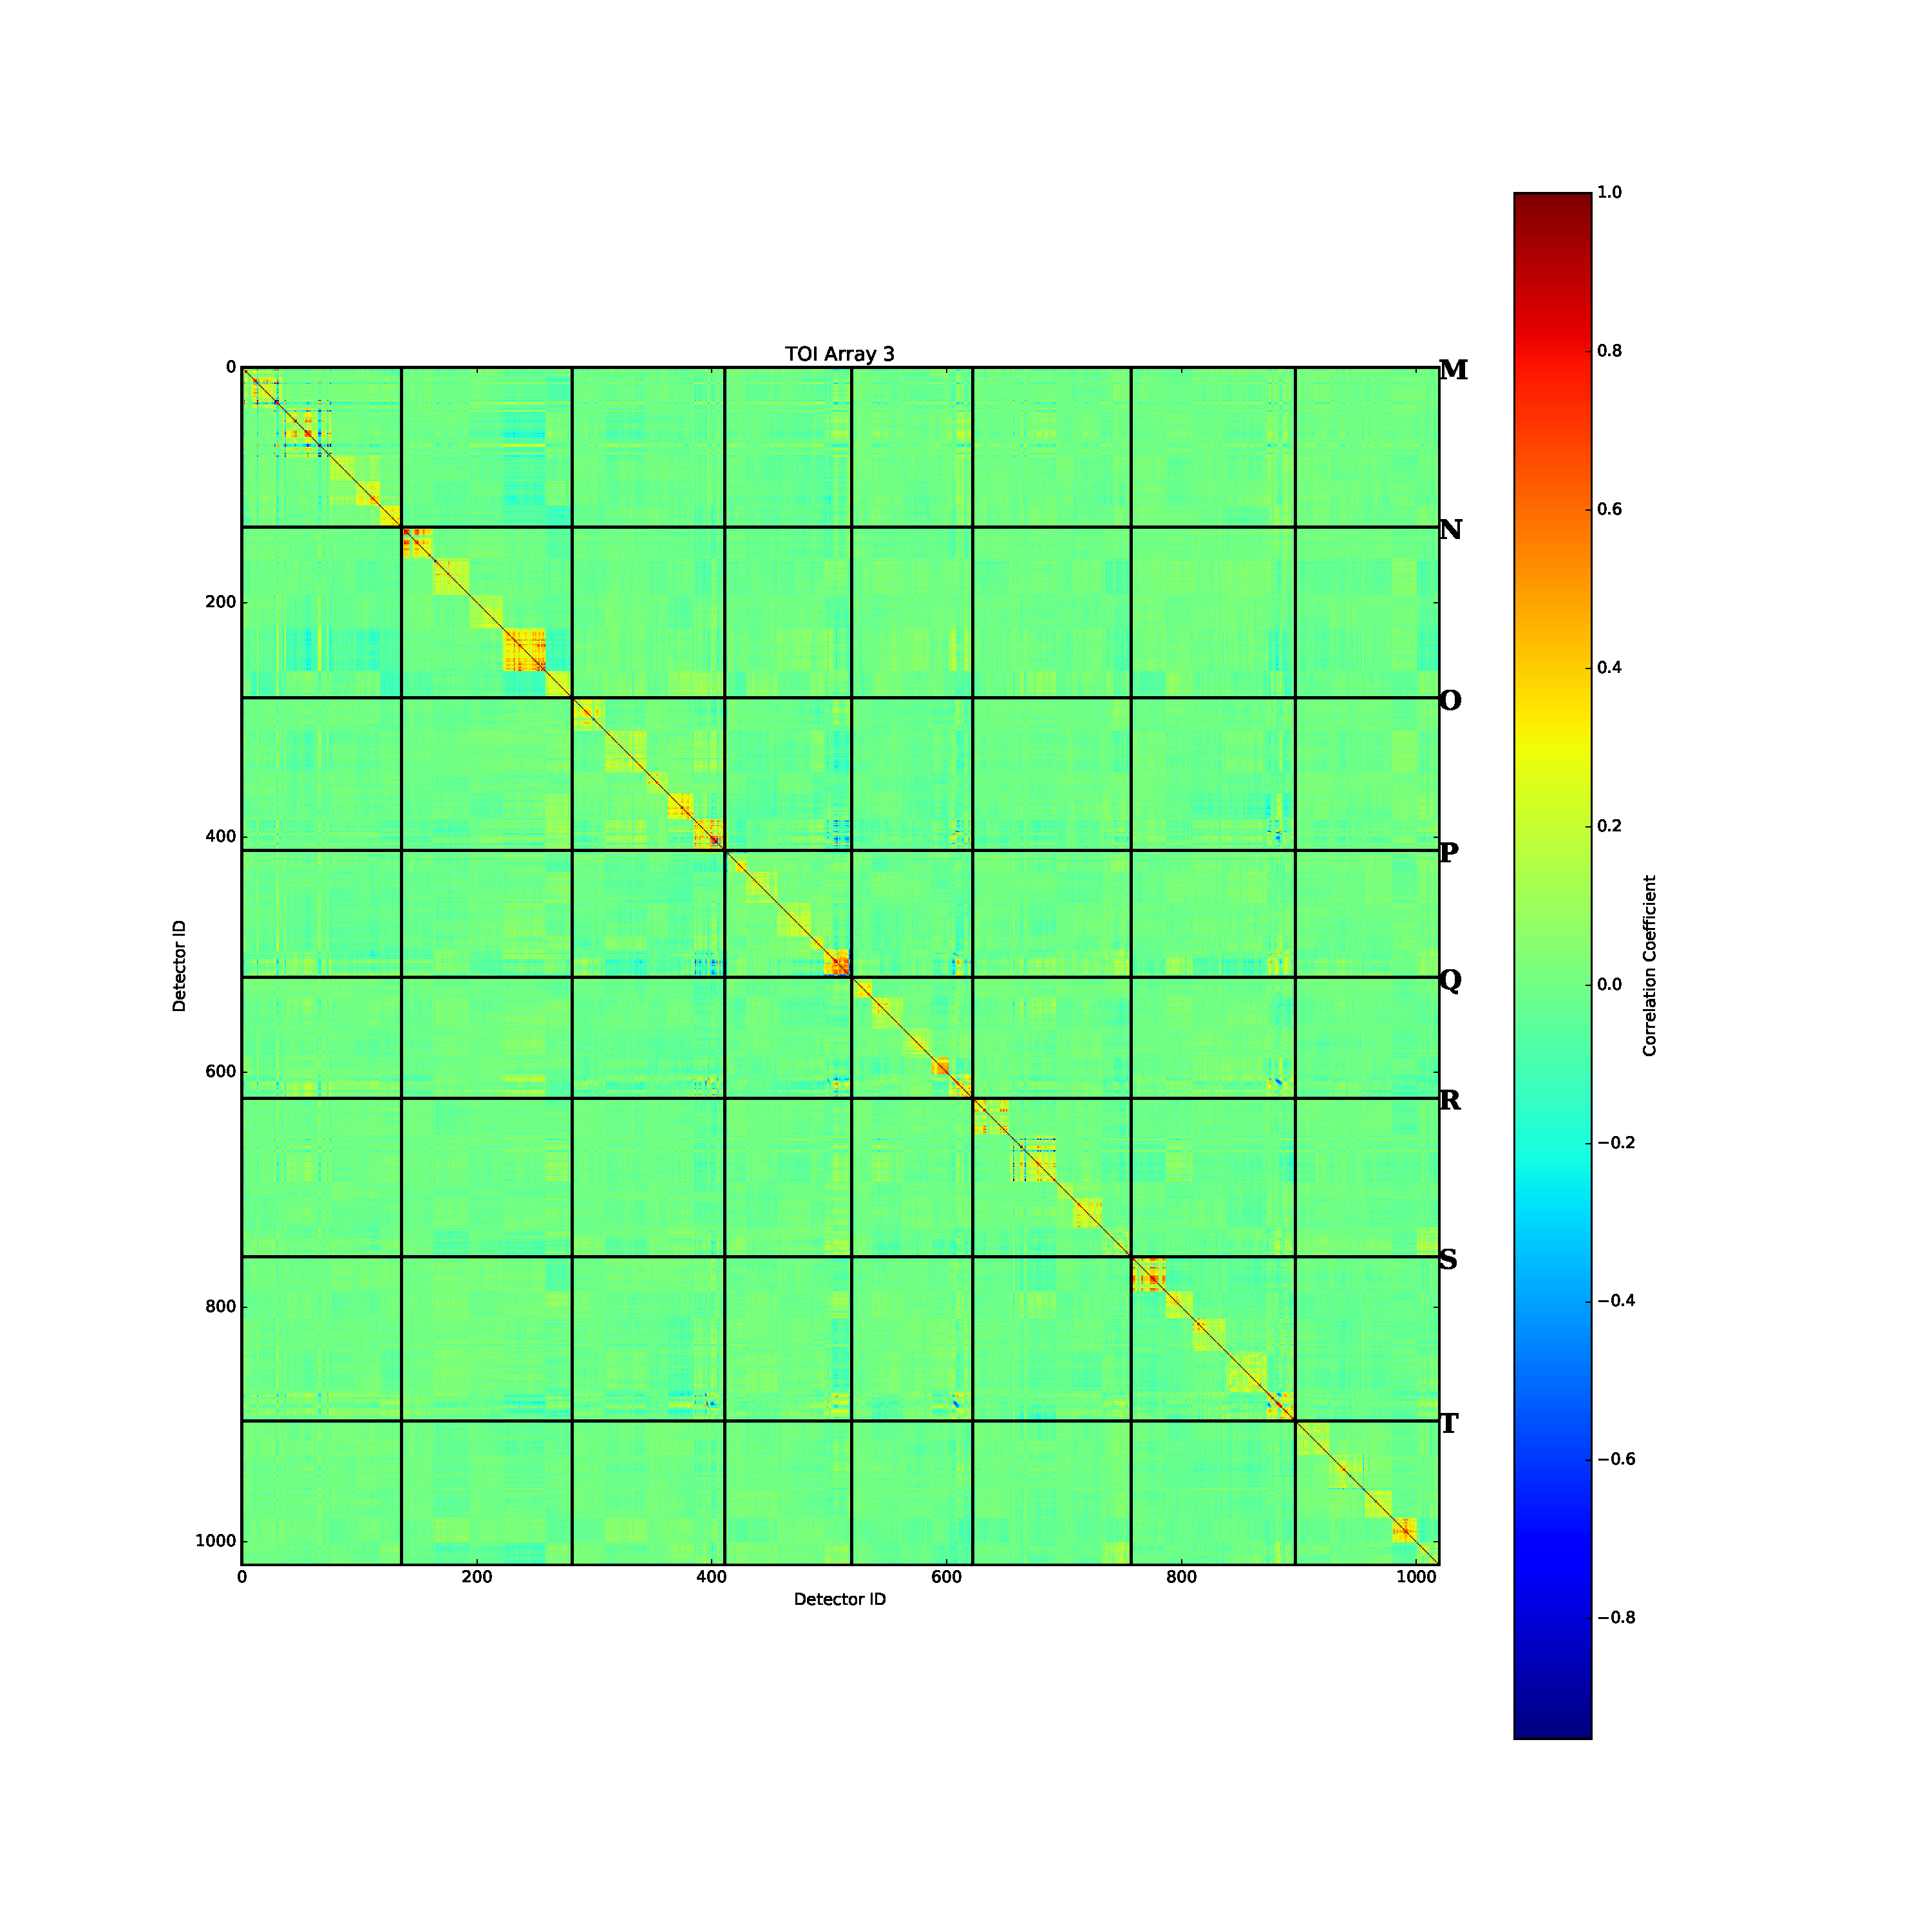
\includegraphics[width=0.3\textwidth]{Figures/DarkTests/corrmat_TOI_PCA_array_3_20161211s299.pdf}
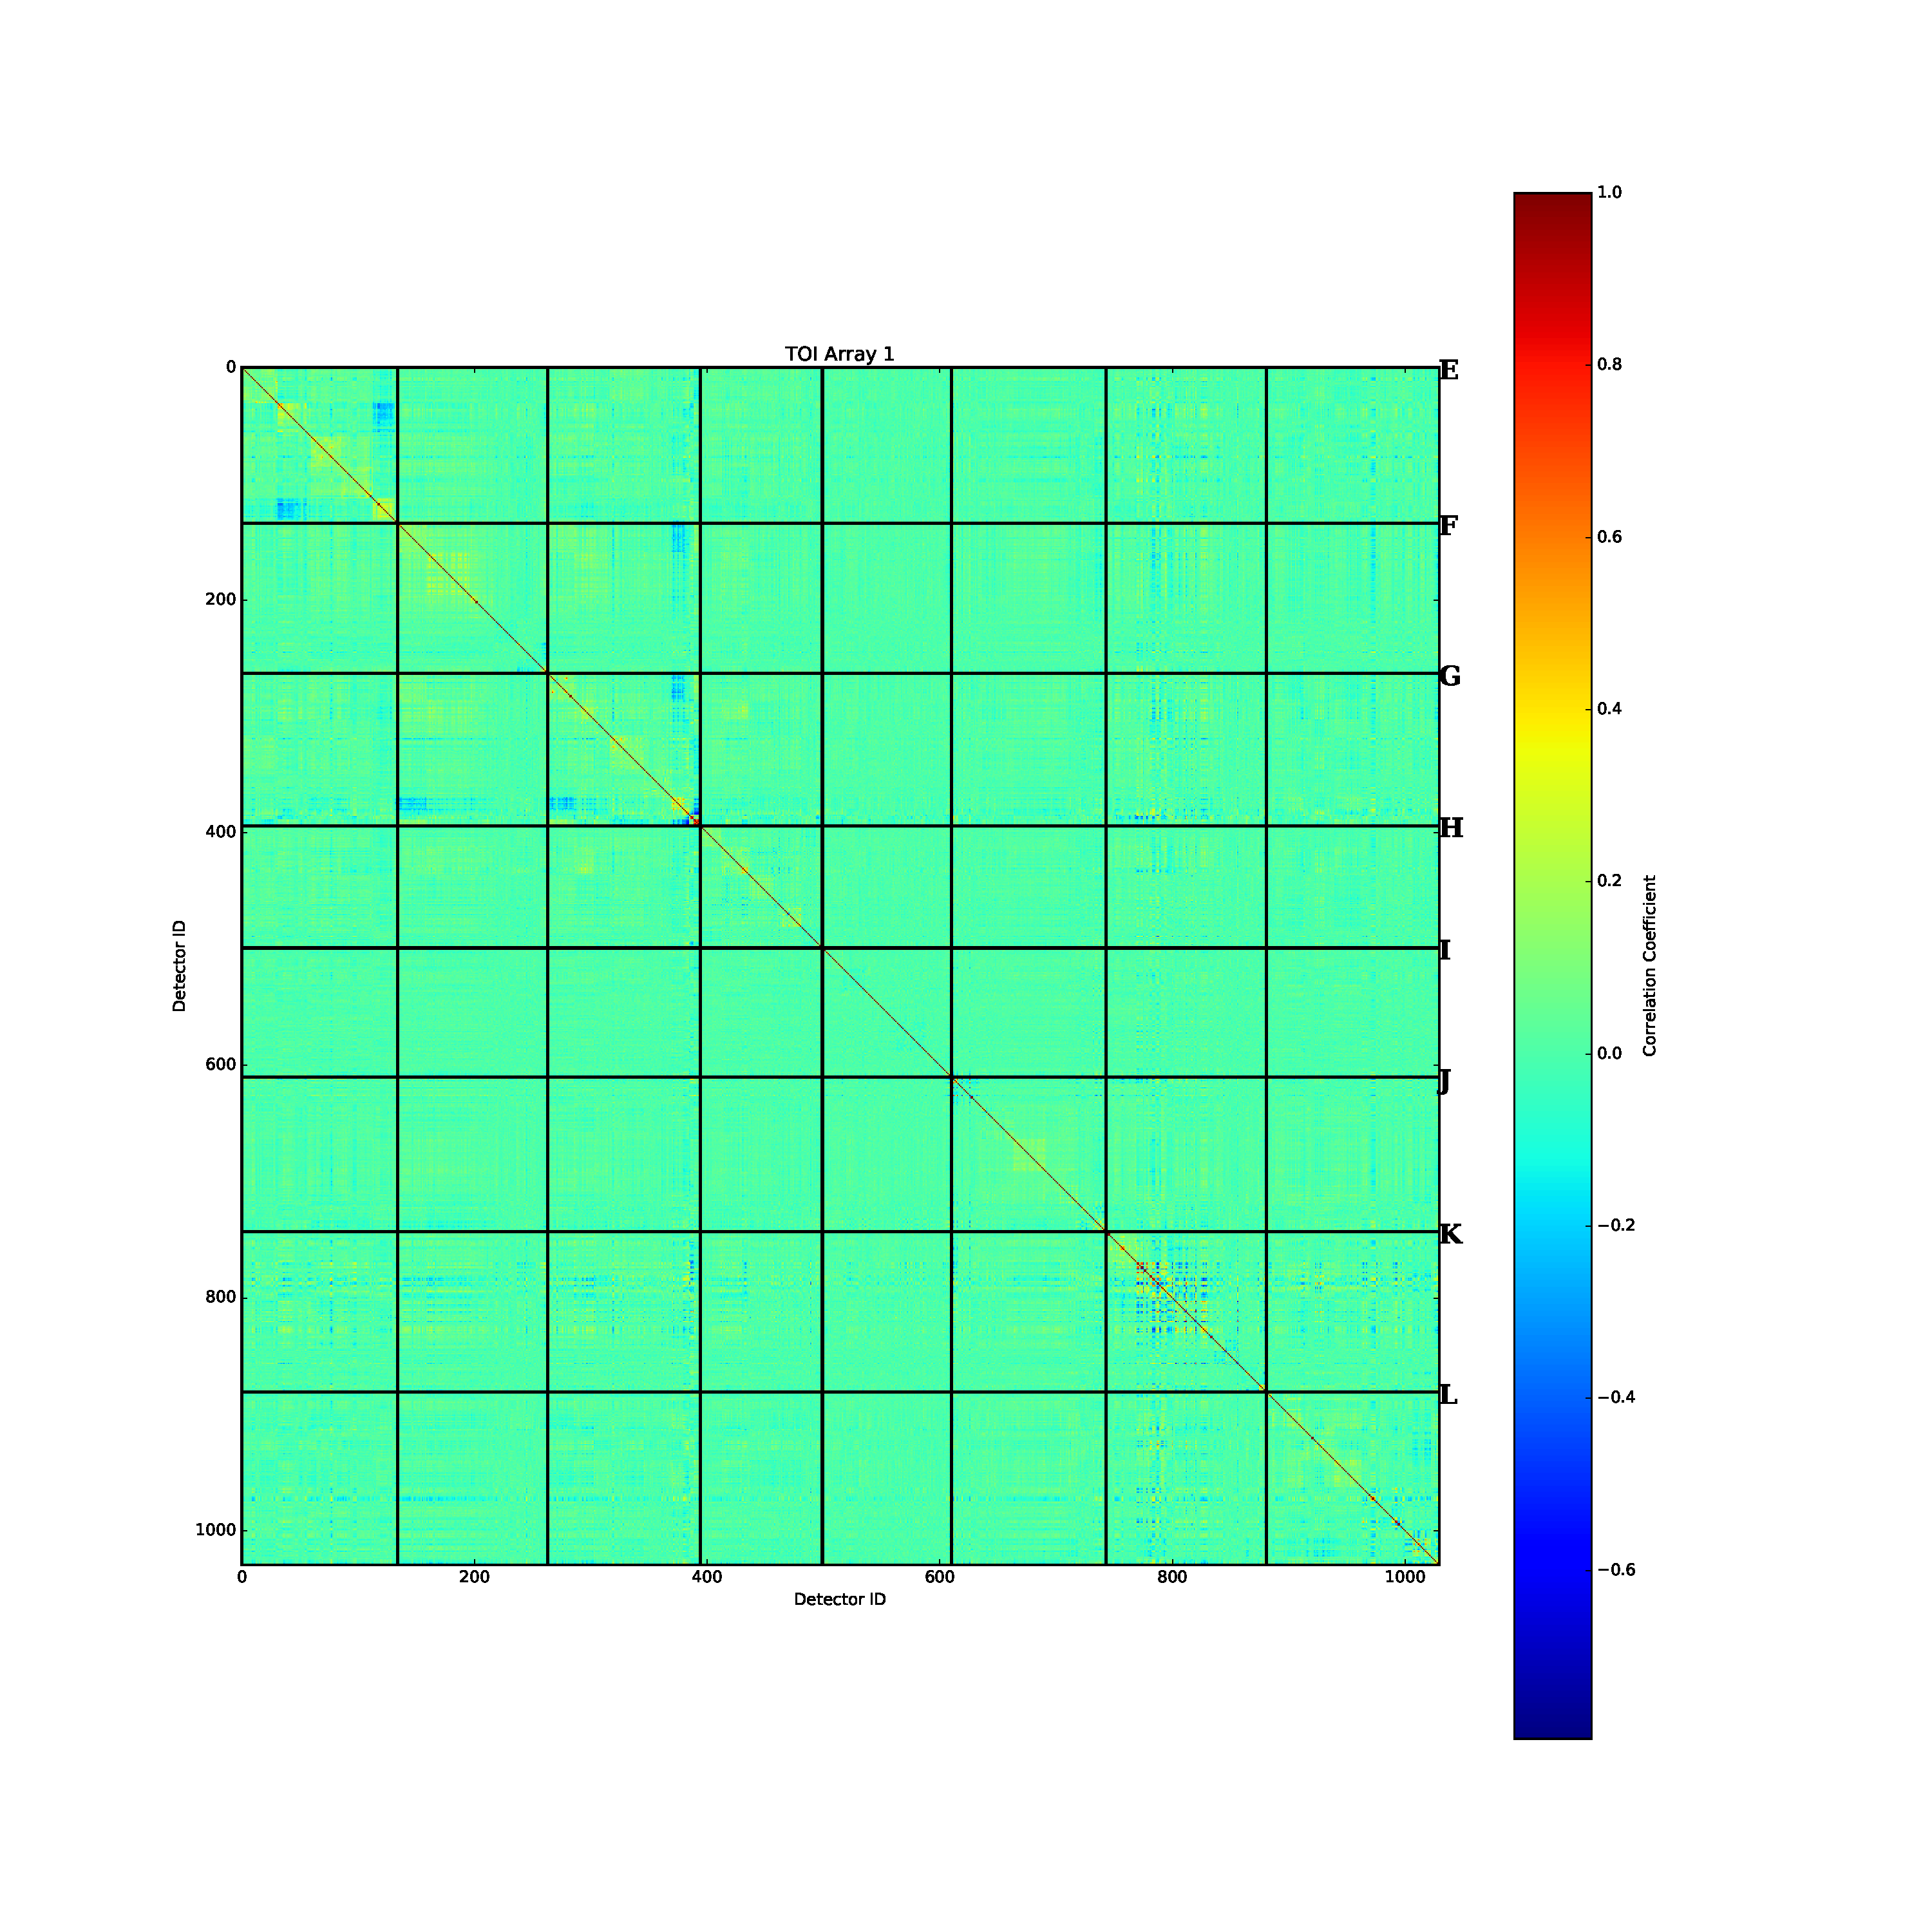
\includegraphics[width=0.3\textwidth]{Figures/DarkTests/corrmat_TOI_BC_array_1_20161211s299.pdf}
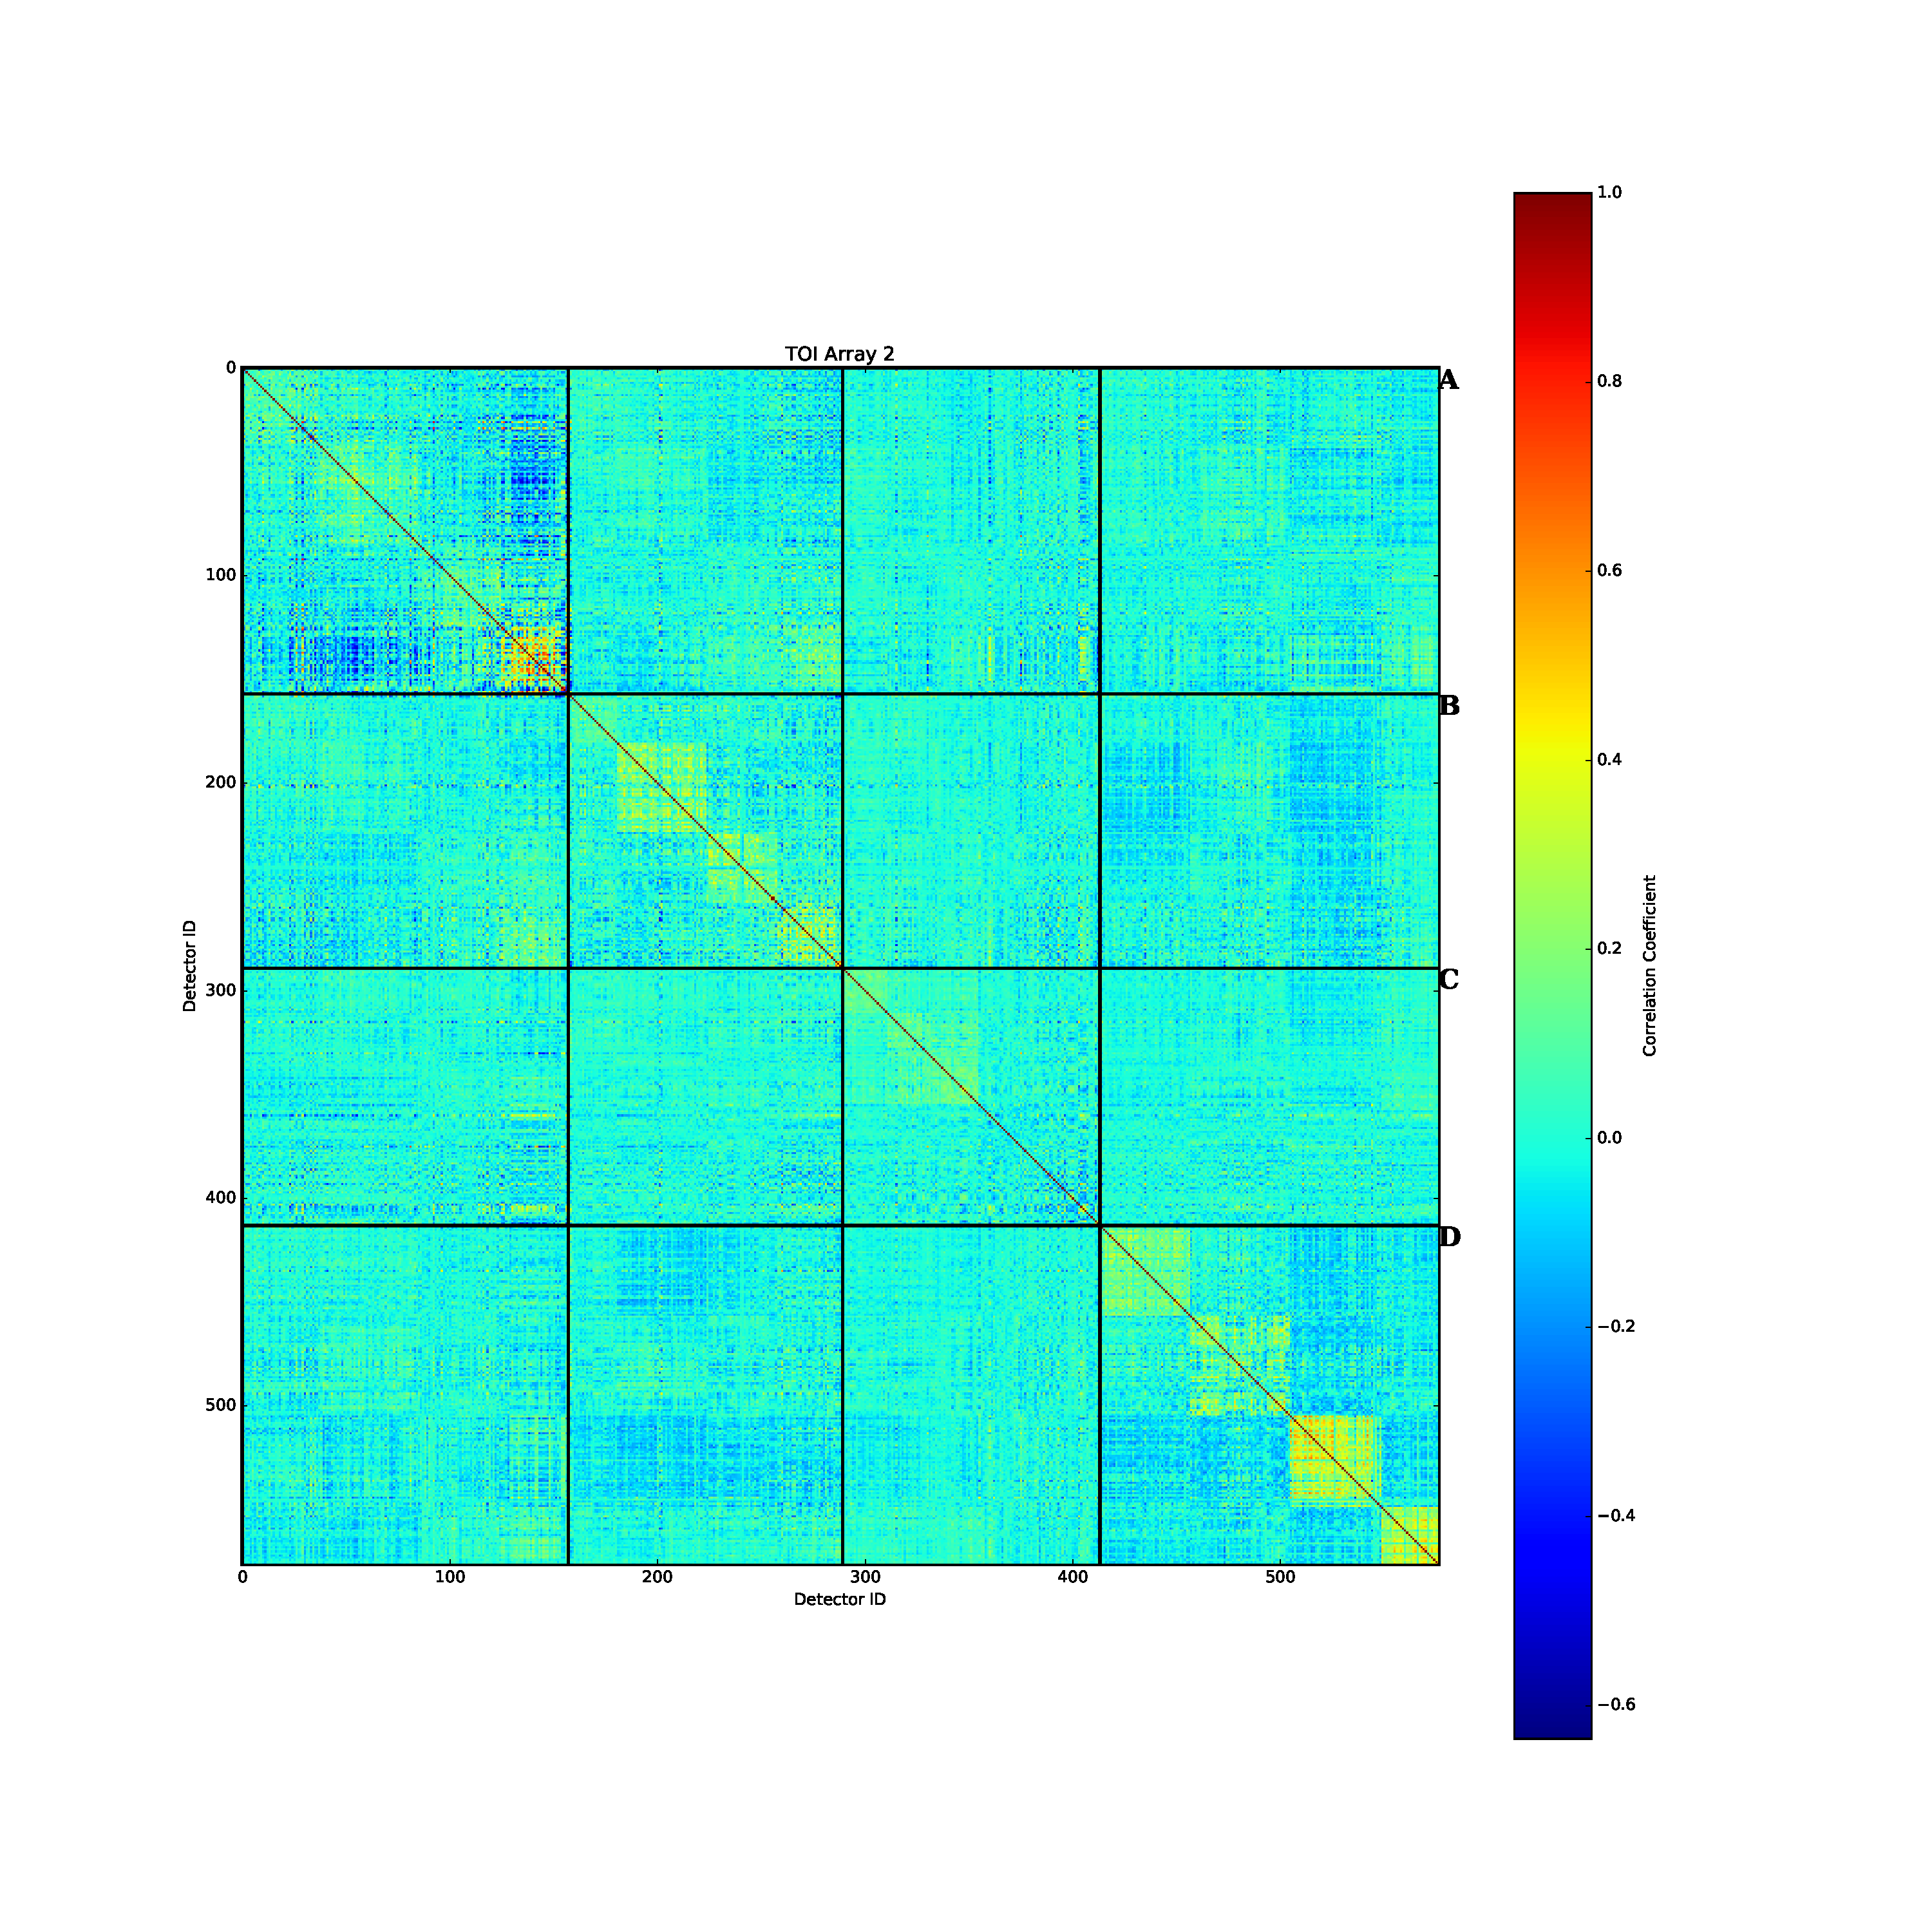
\includegraphics[width=0.3\textwidth]{Figures/DarkTests/corrmat_TOI_BC_array_2_20161211s299.pdf}
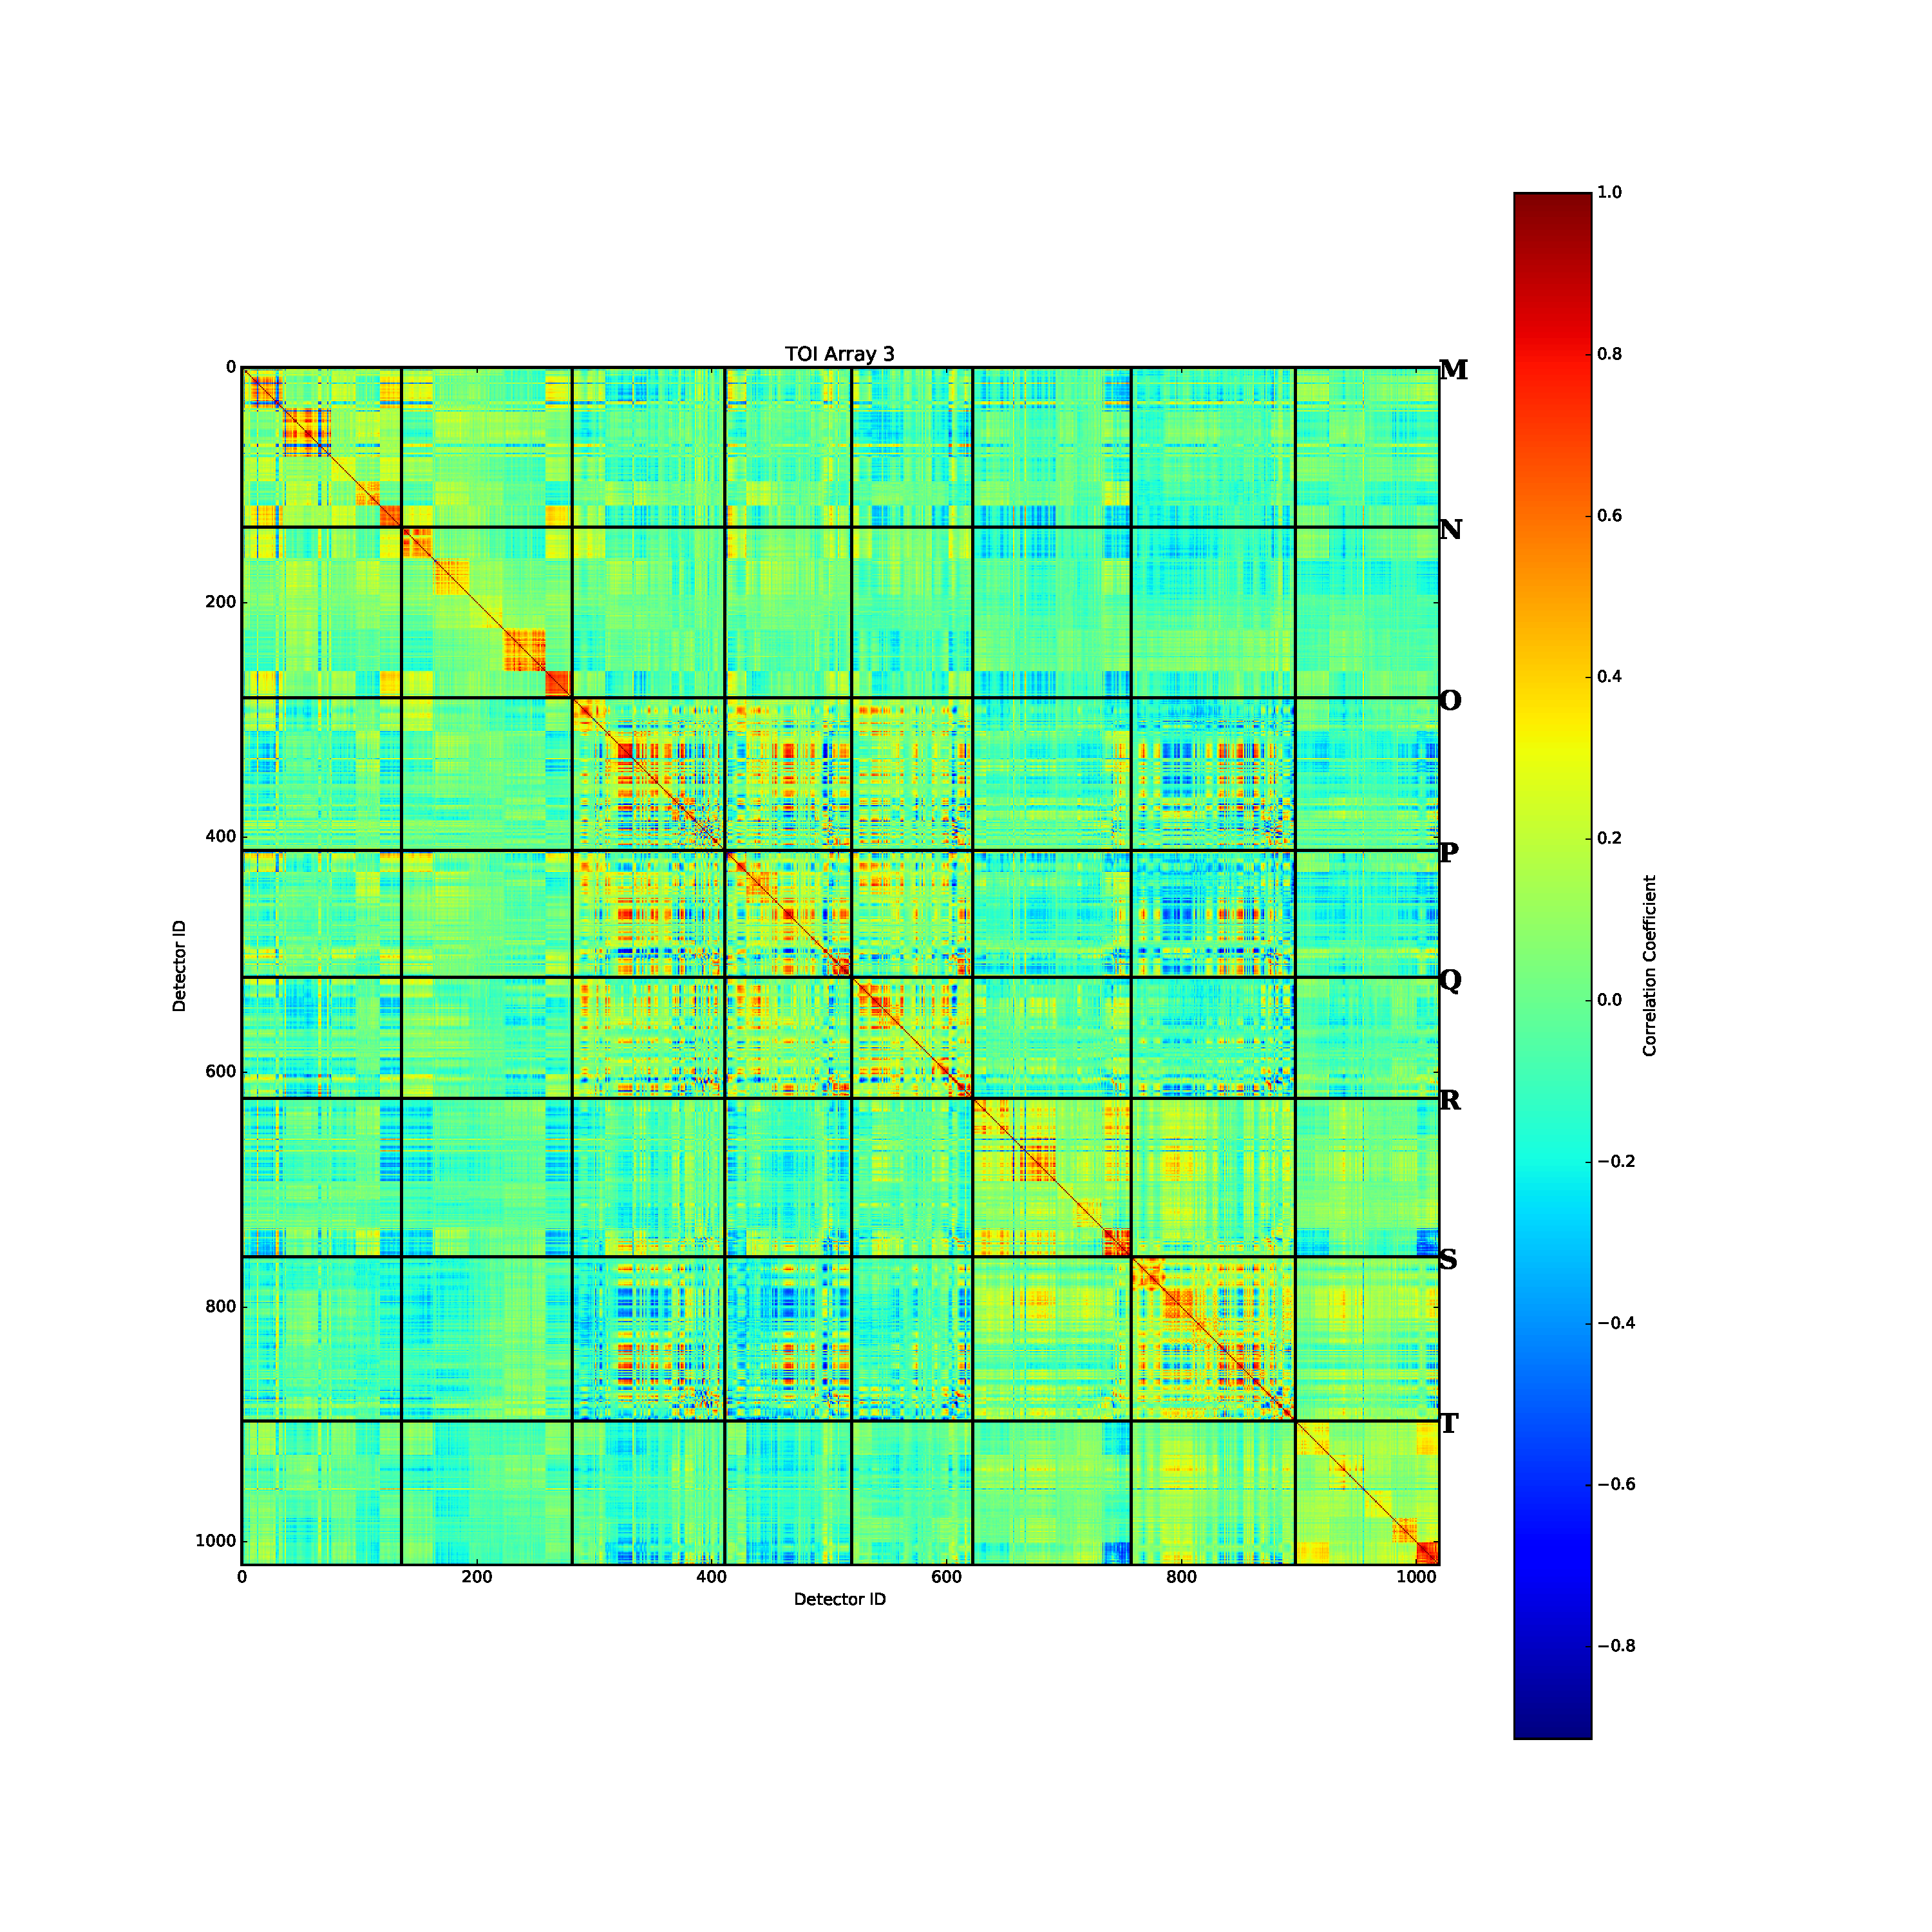
\includegraphics[width=0.3\textwidth]{Figures/DarkTests/corrmat_TOI_BC_array_3_20161211s299.pdf}
\end{center}
\caption{From left to right correlation matrices for the three NIKA2 arrays (A1, A2, and A3) for scan 20161211s299. From top to bottom we present the correlation of the raw data, after CM, PCA and BC decorrelations. \label{corrs299}}
\end{figure}



\begin{figure}[ht] % Inline image example
\begin{center}
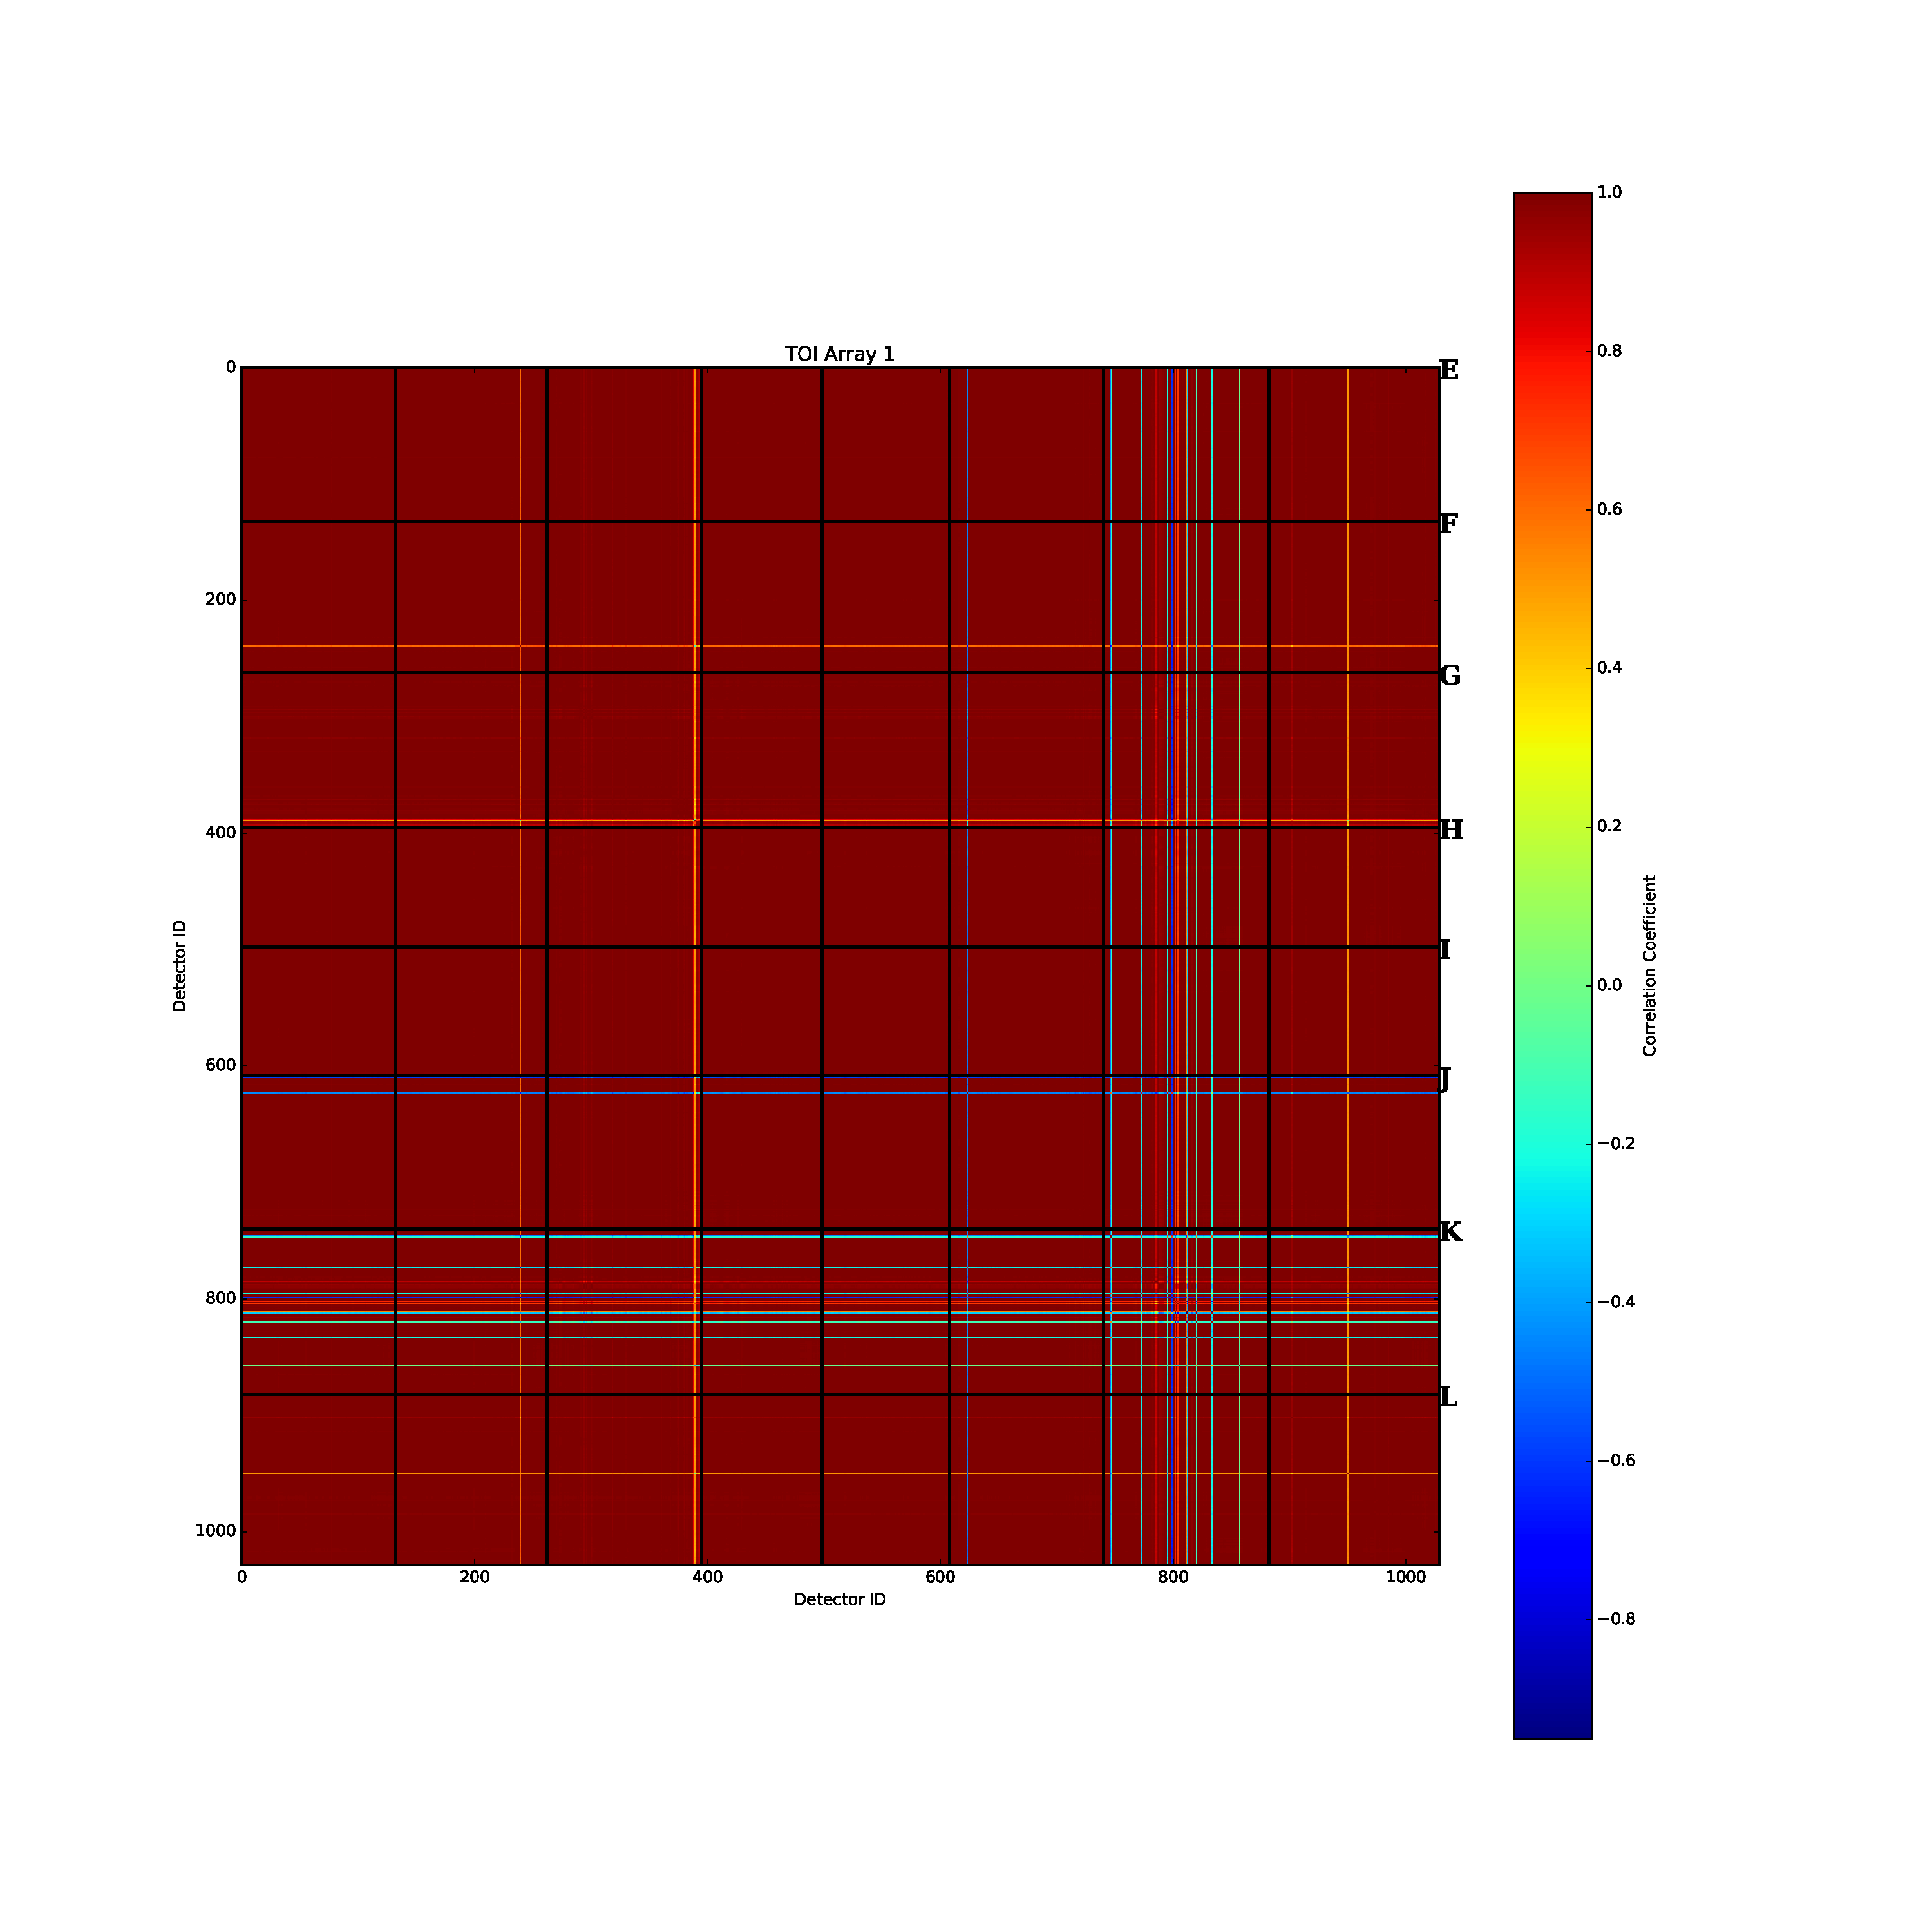
\includegraphics[width=0.3\textwidth]{Figures/DarkTests/corrmat_TOI_array_1_20161213s72.pdf}
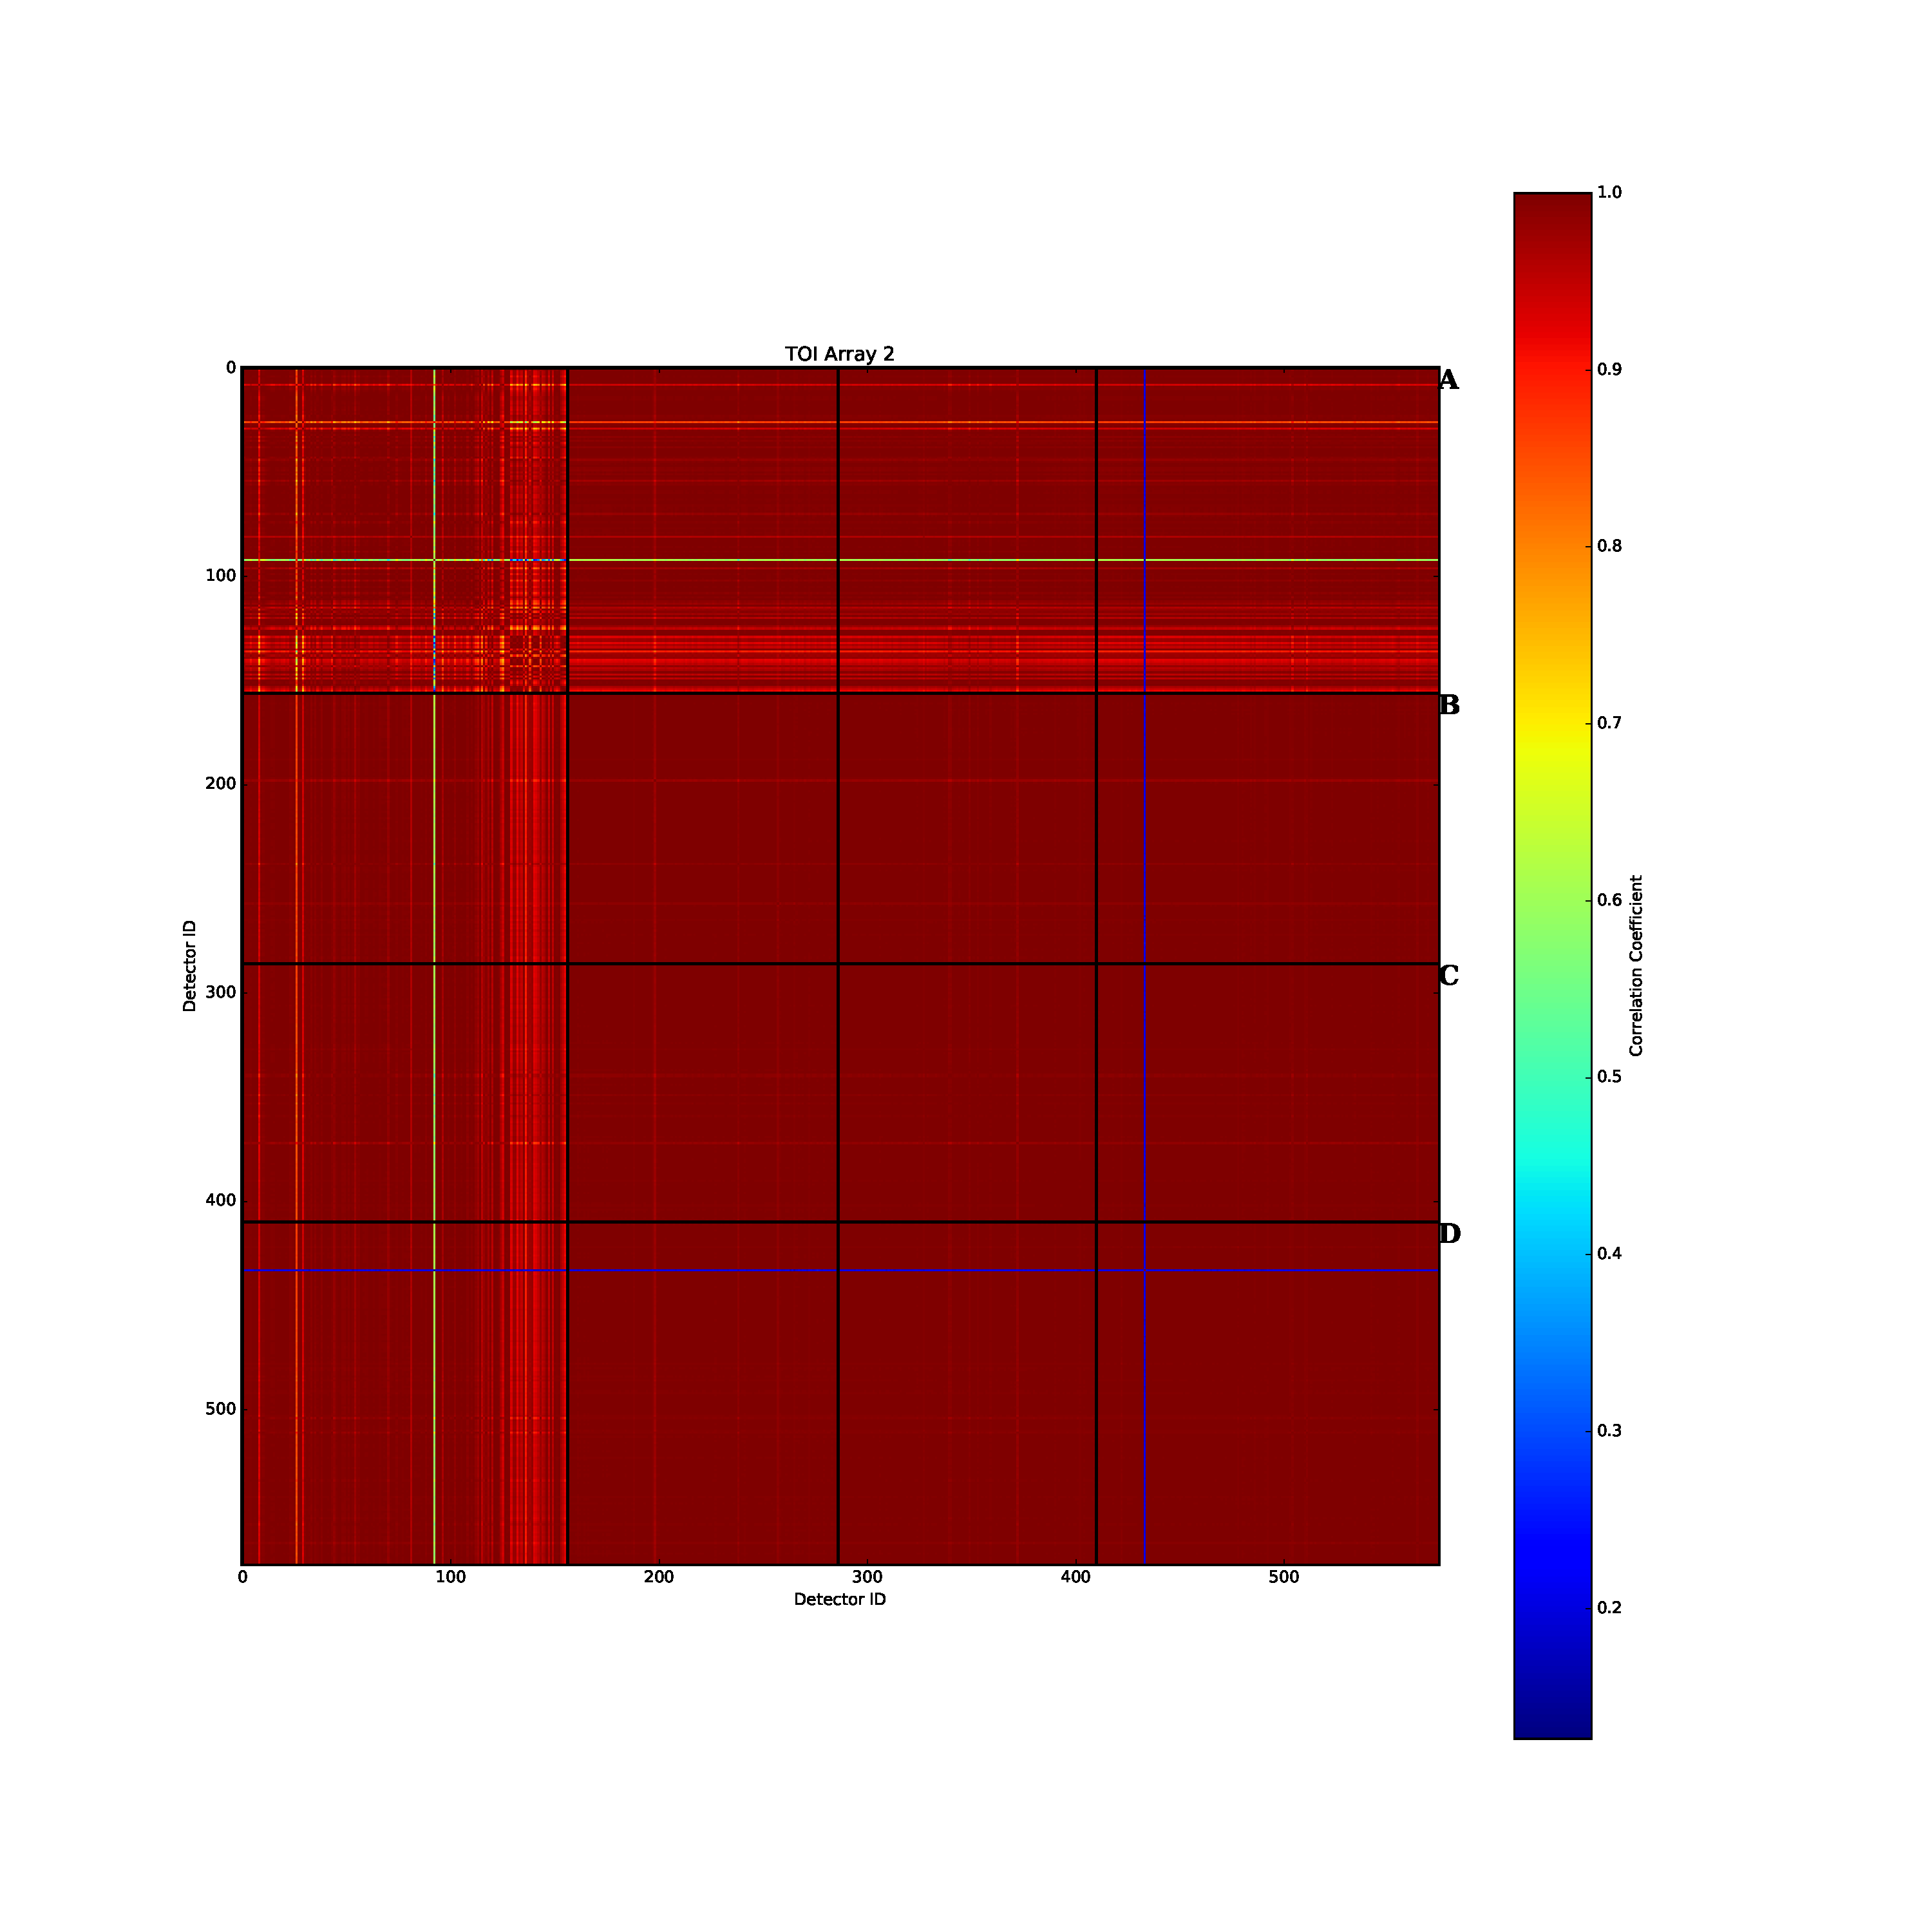
\includegraphics[width=0.3\textwidth]{Figures/DarkTests/corrmat_TOI_array_2_20161213s72.pdf}
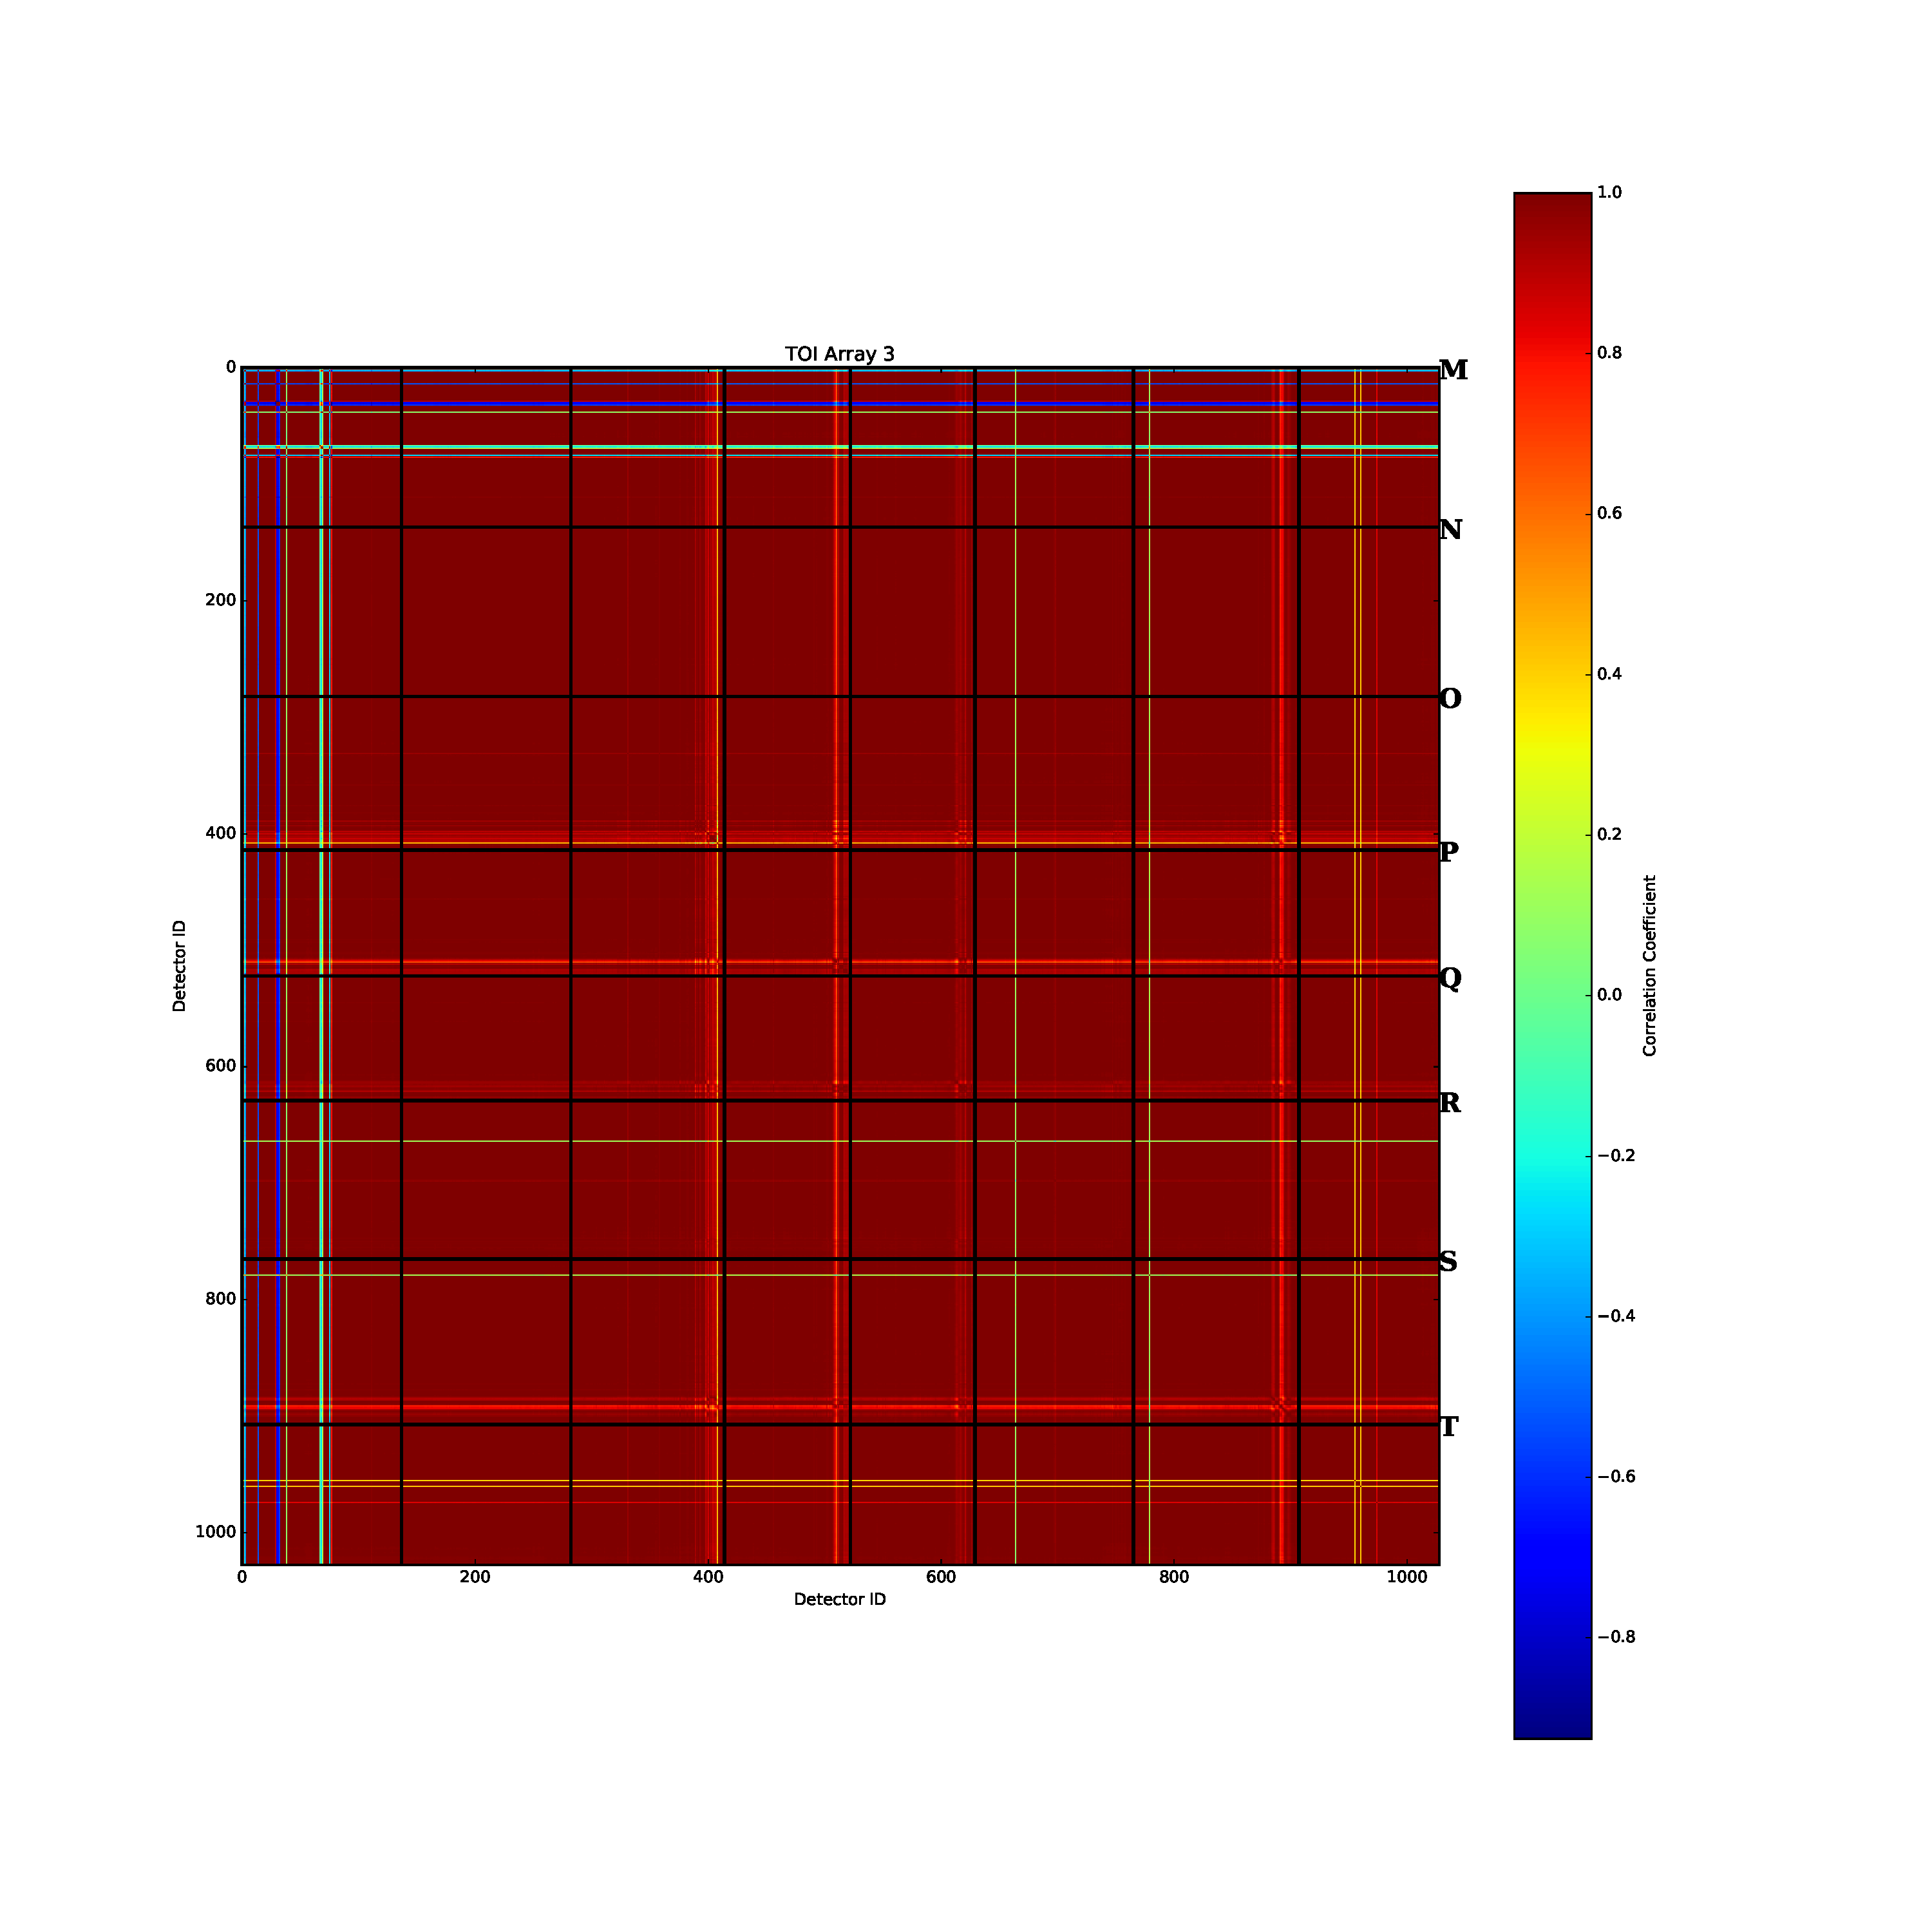
\includegraphics[width=0.3\textwidth]{Figures/DarkTests/corrmat_TOI_array_3_20161213s72.pdf}
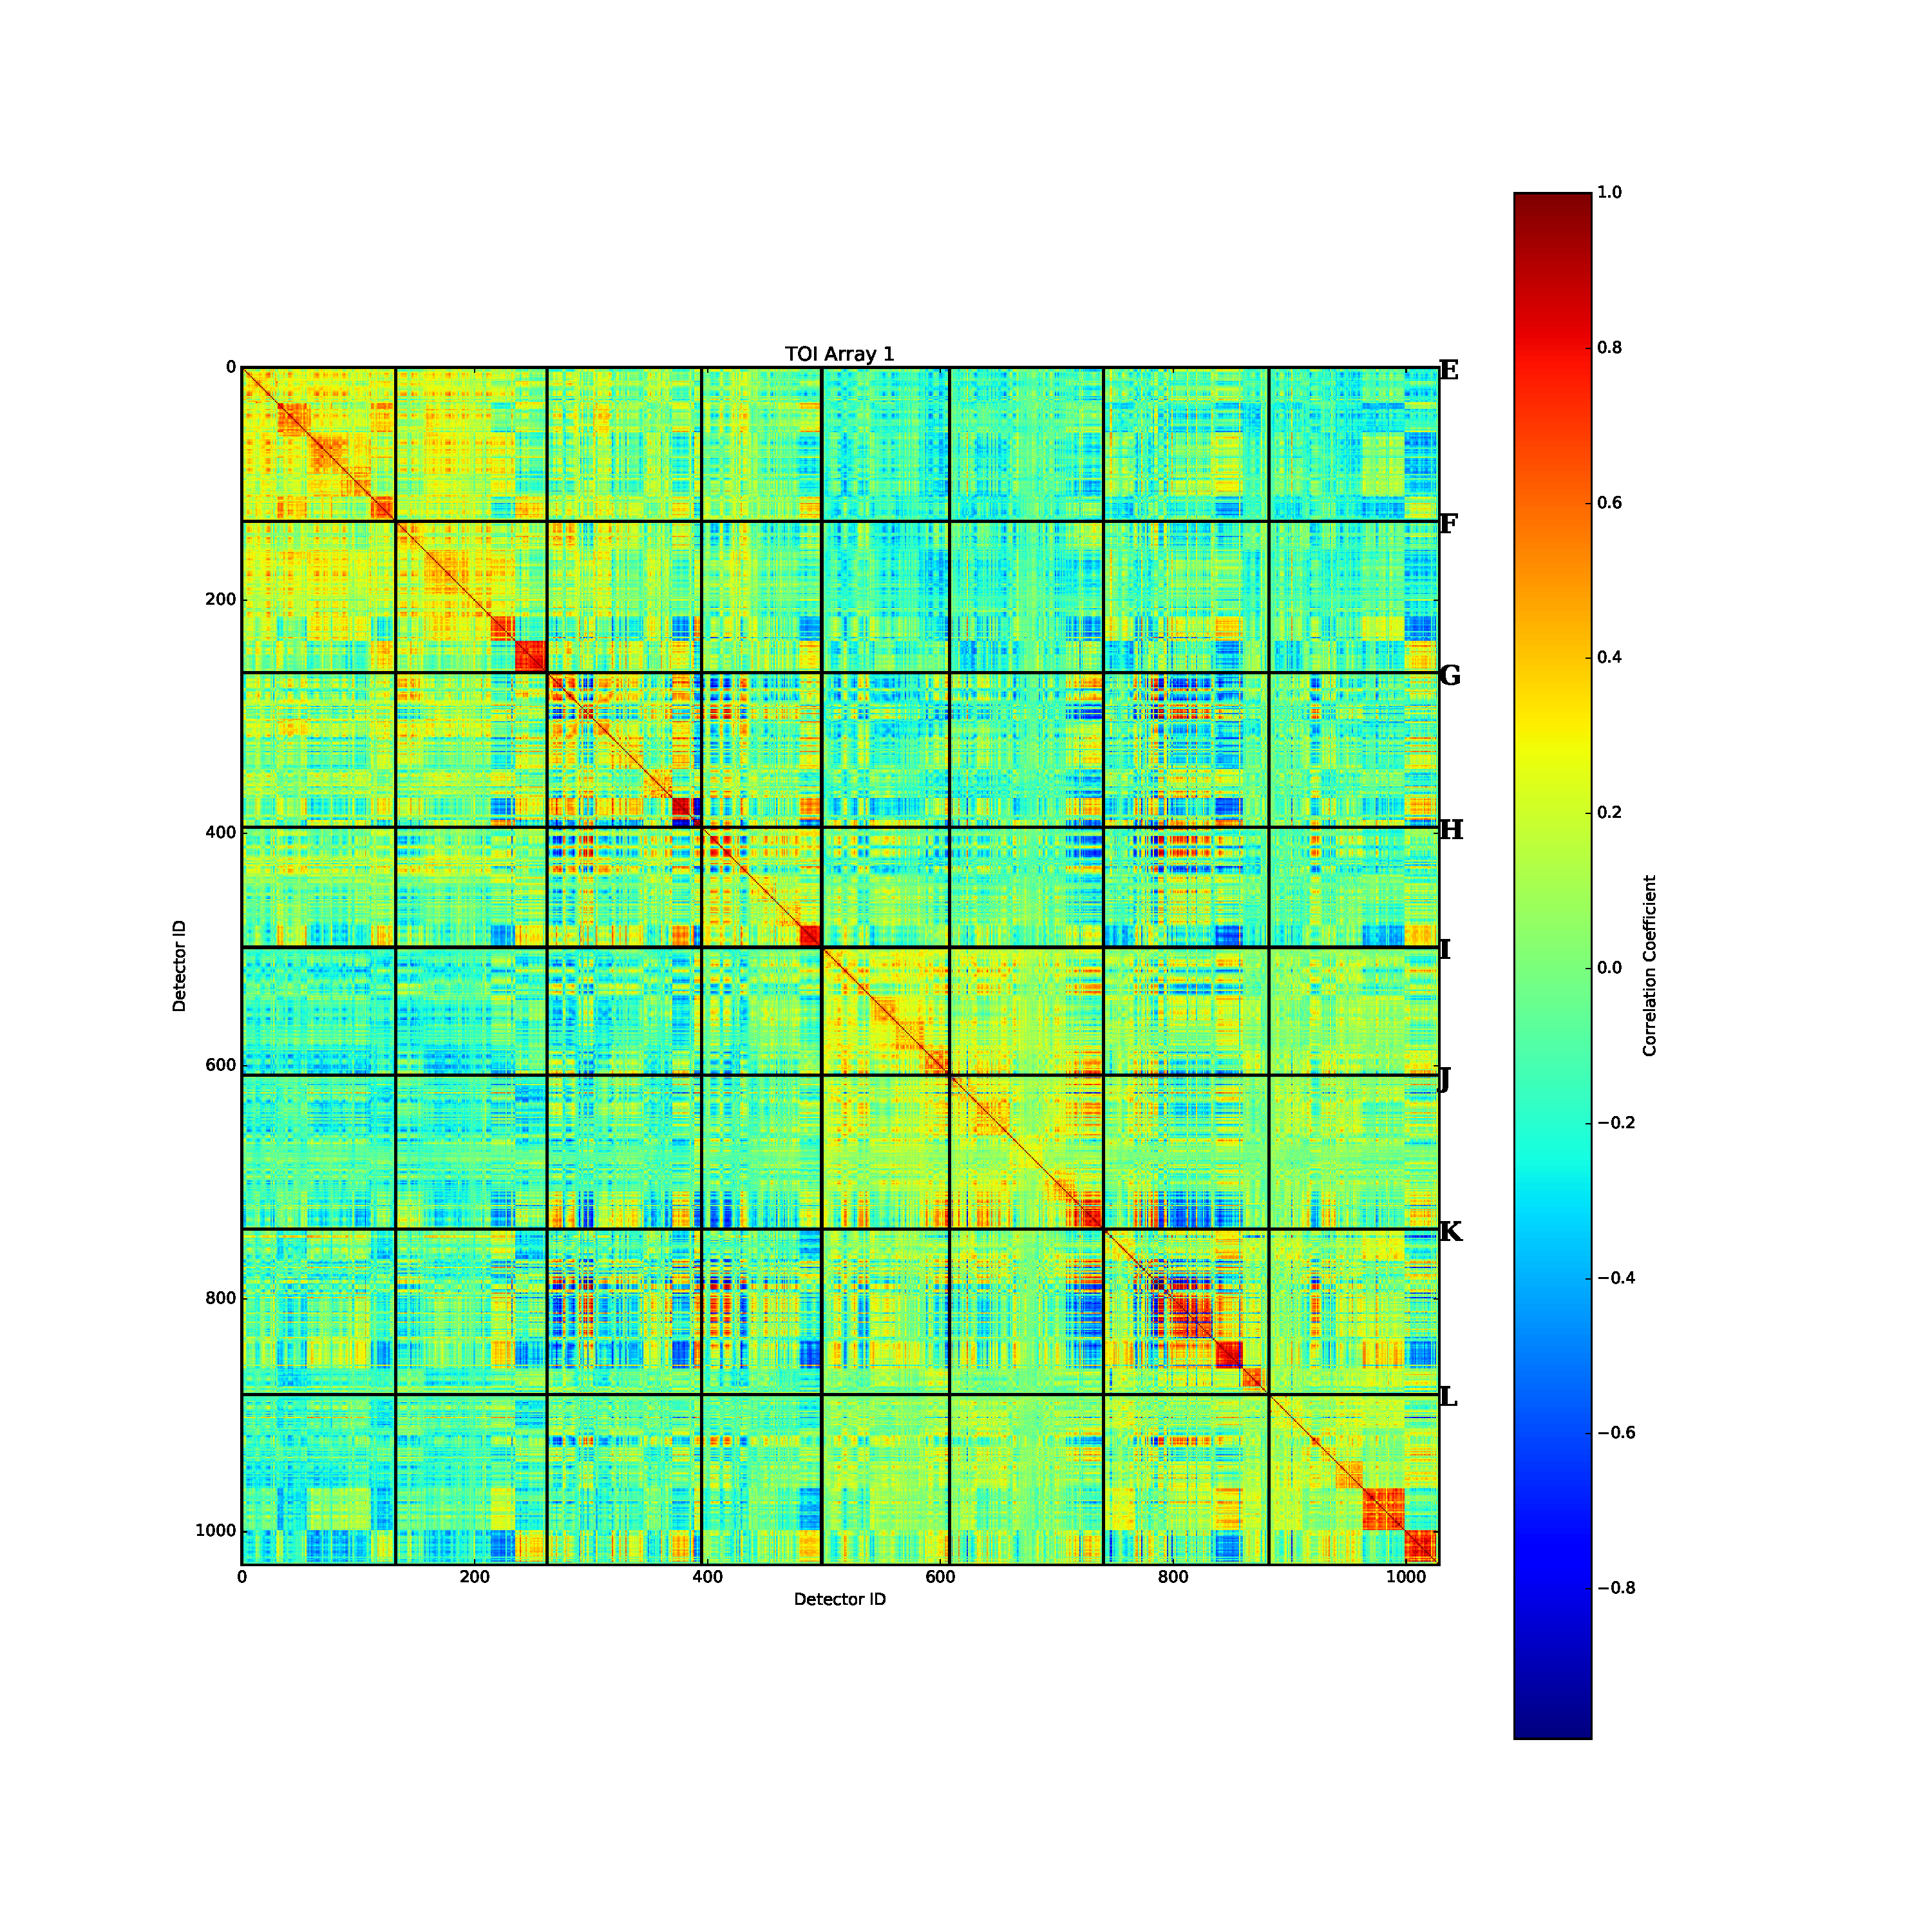
\includegraphics[width=0.3\textwidth]{Figures/DarkTests/corrmat_TOI_CM_array_1_20161213s72.pdf}
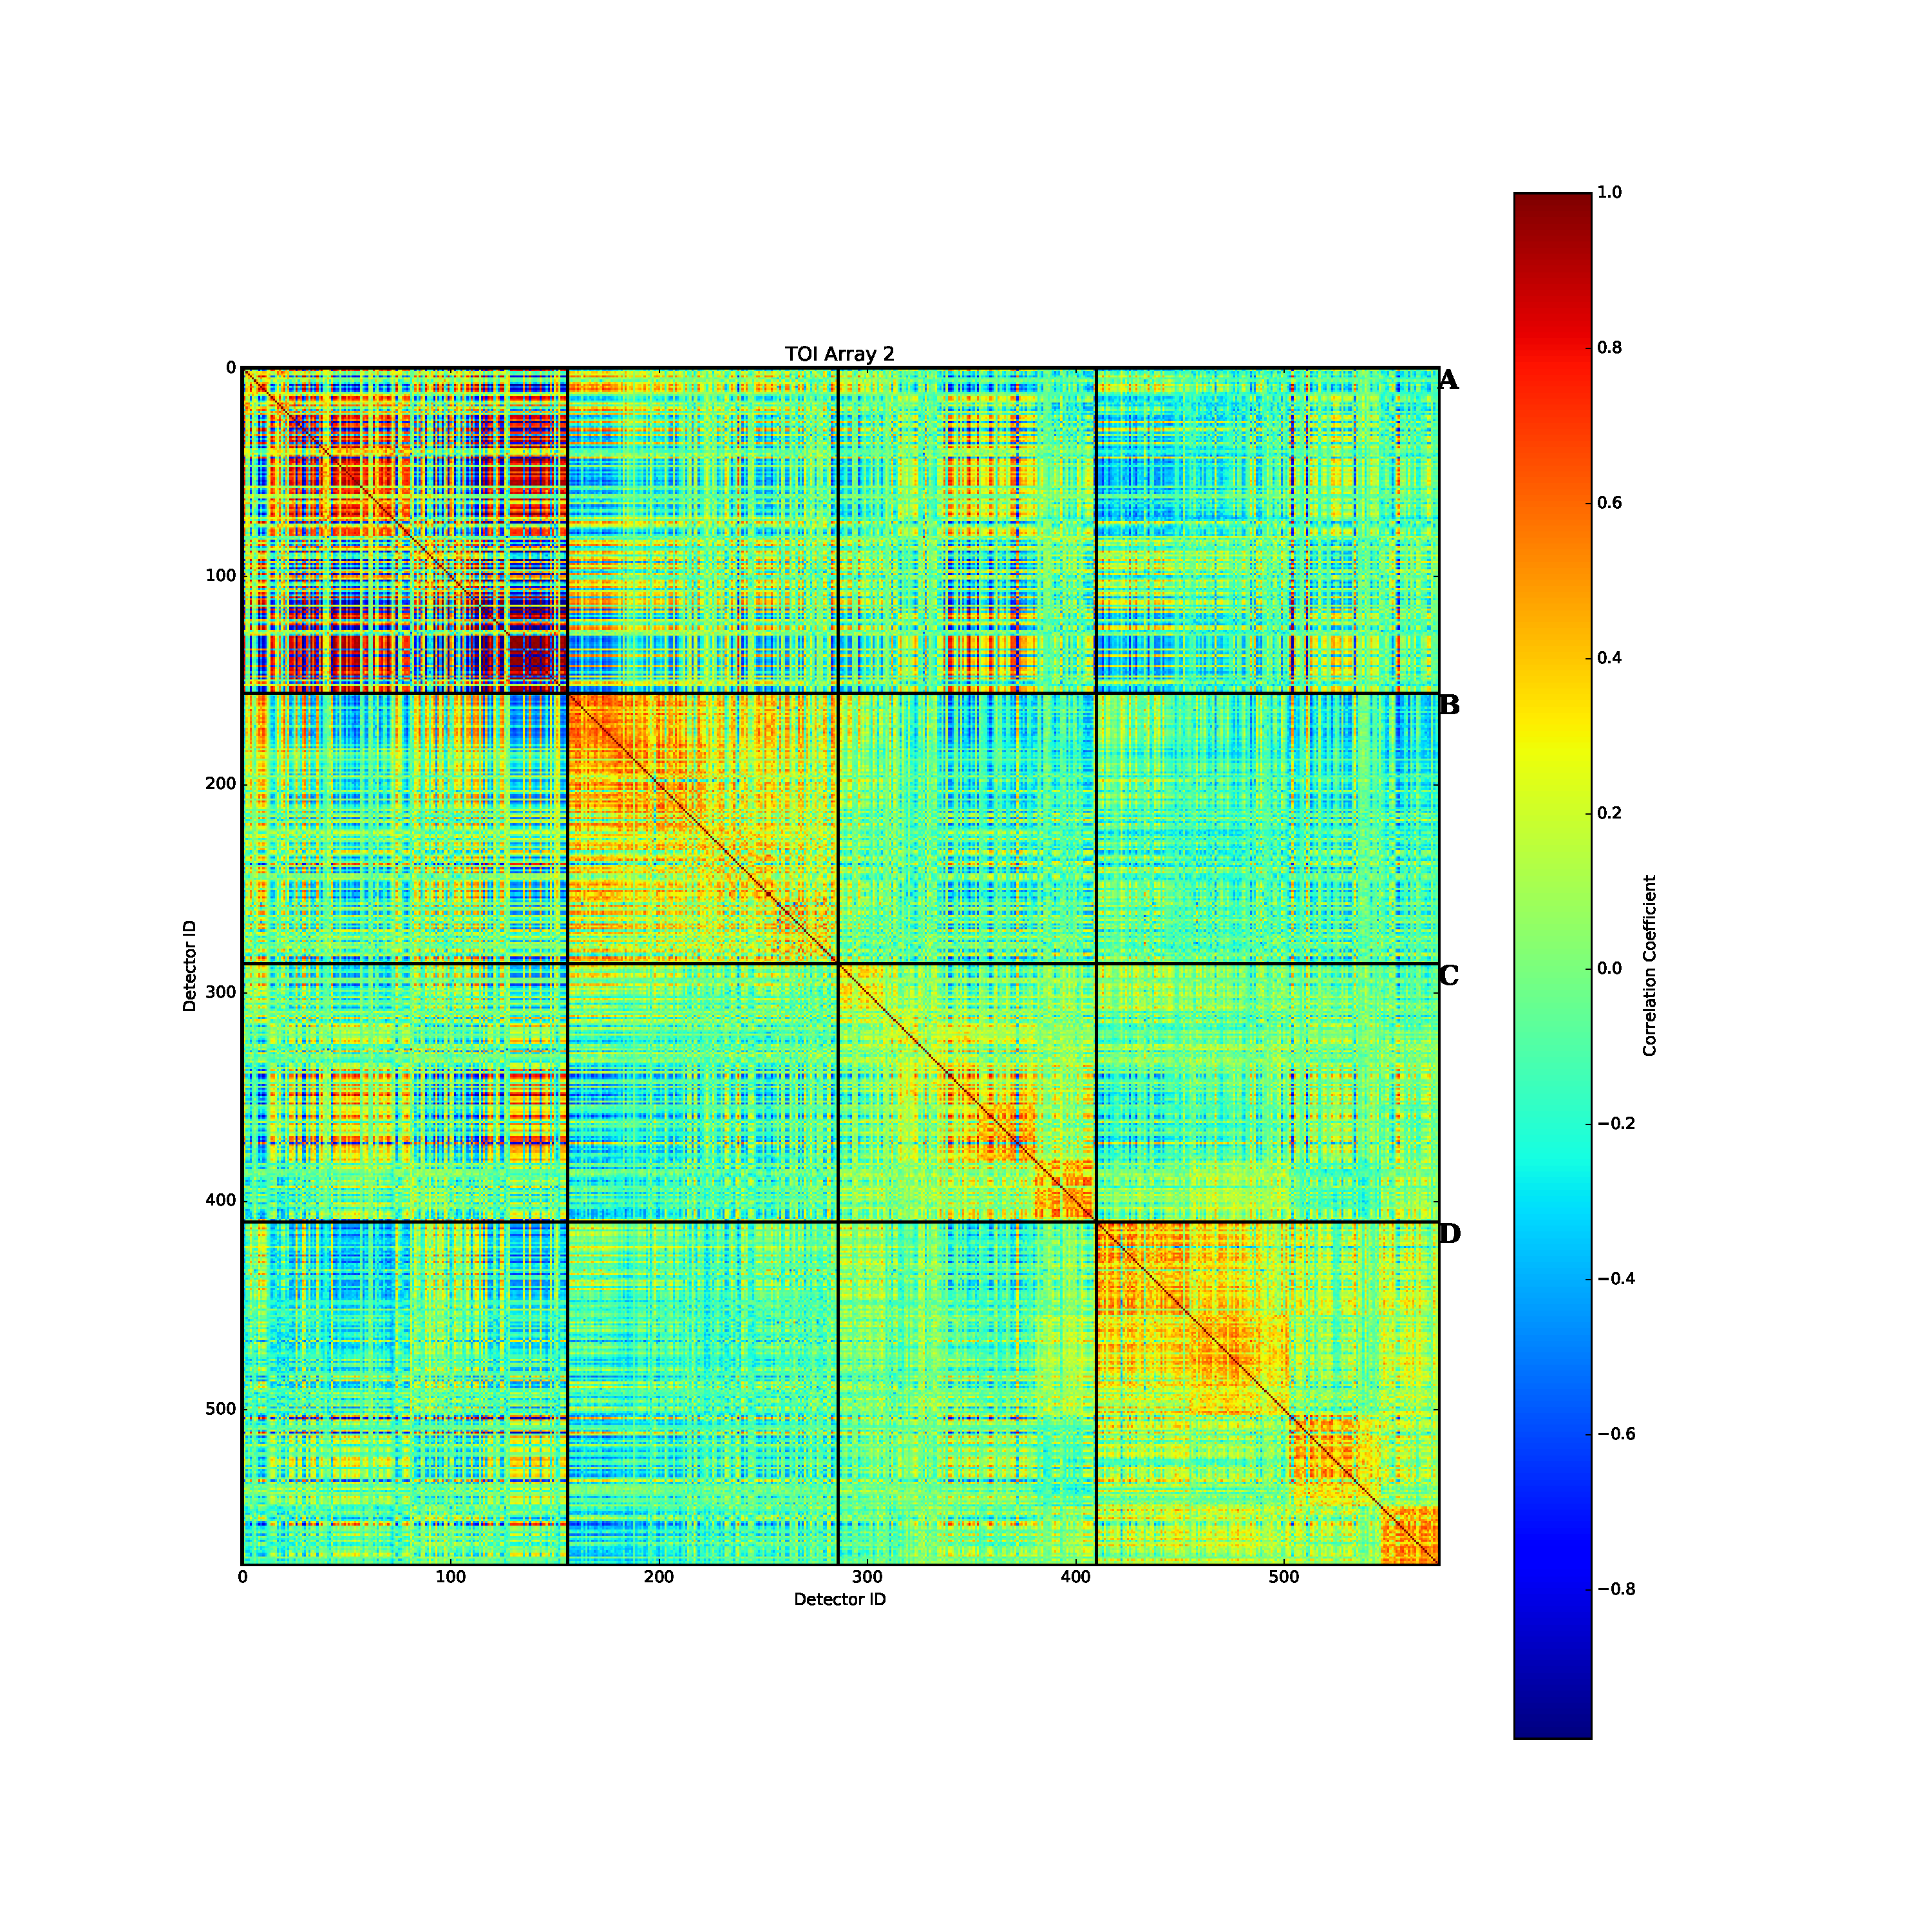
\includegraphics[width=0.3\textwidth]{Figures/DarkTests/corrmat_TOI_CM_array_2_20161213s72.pdf}
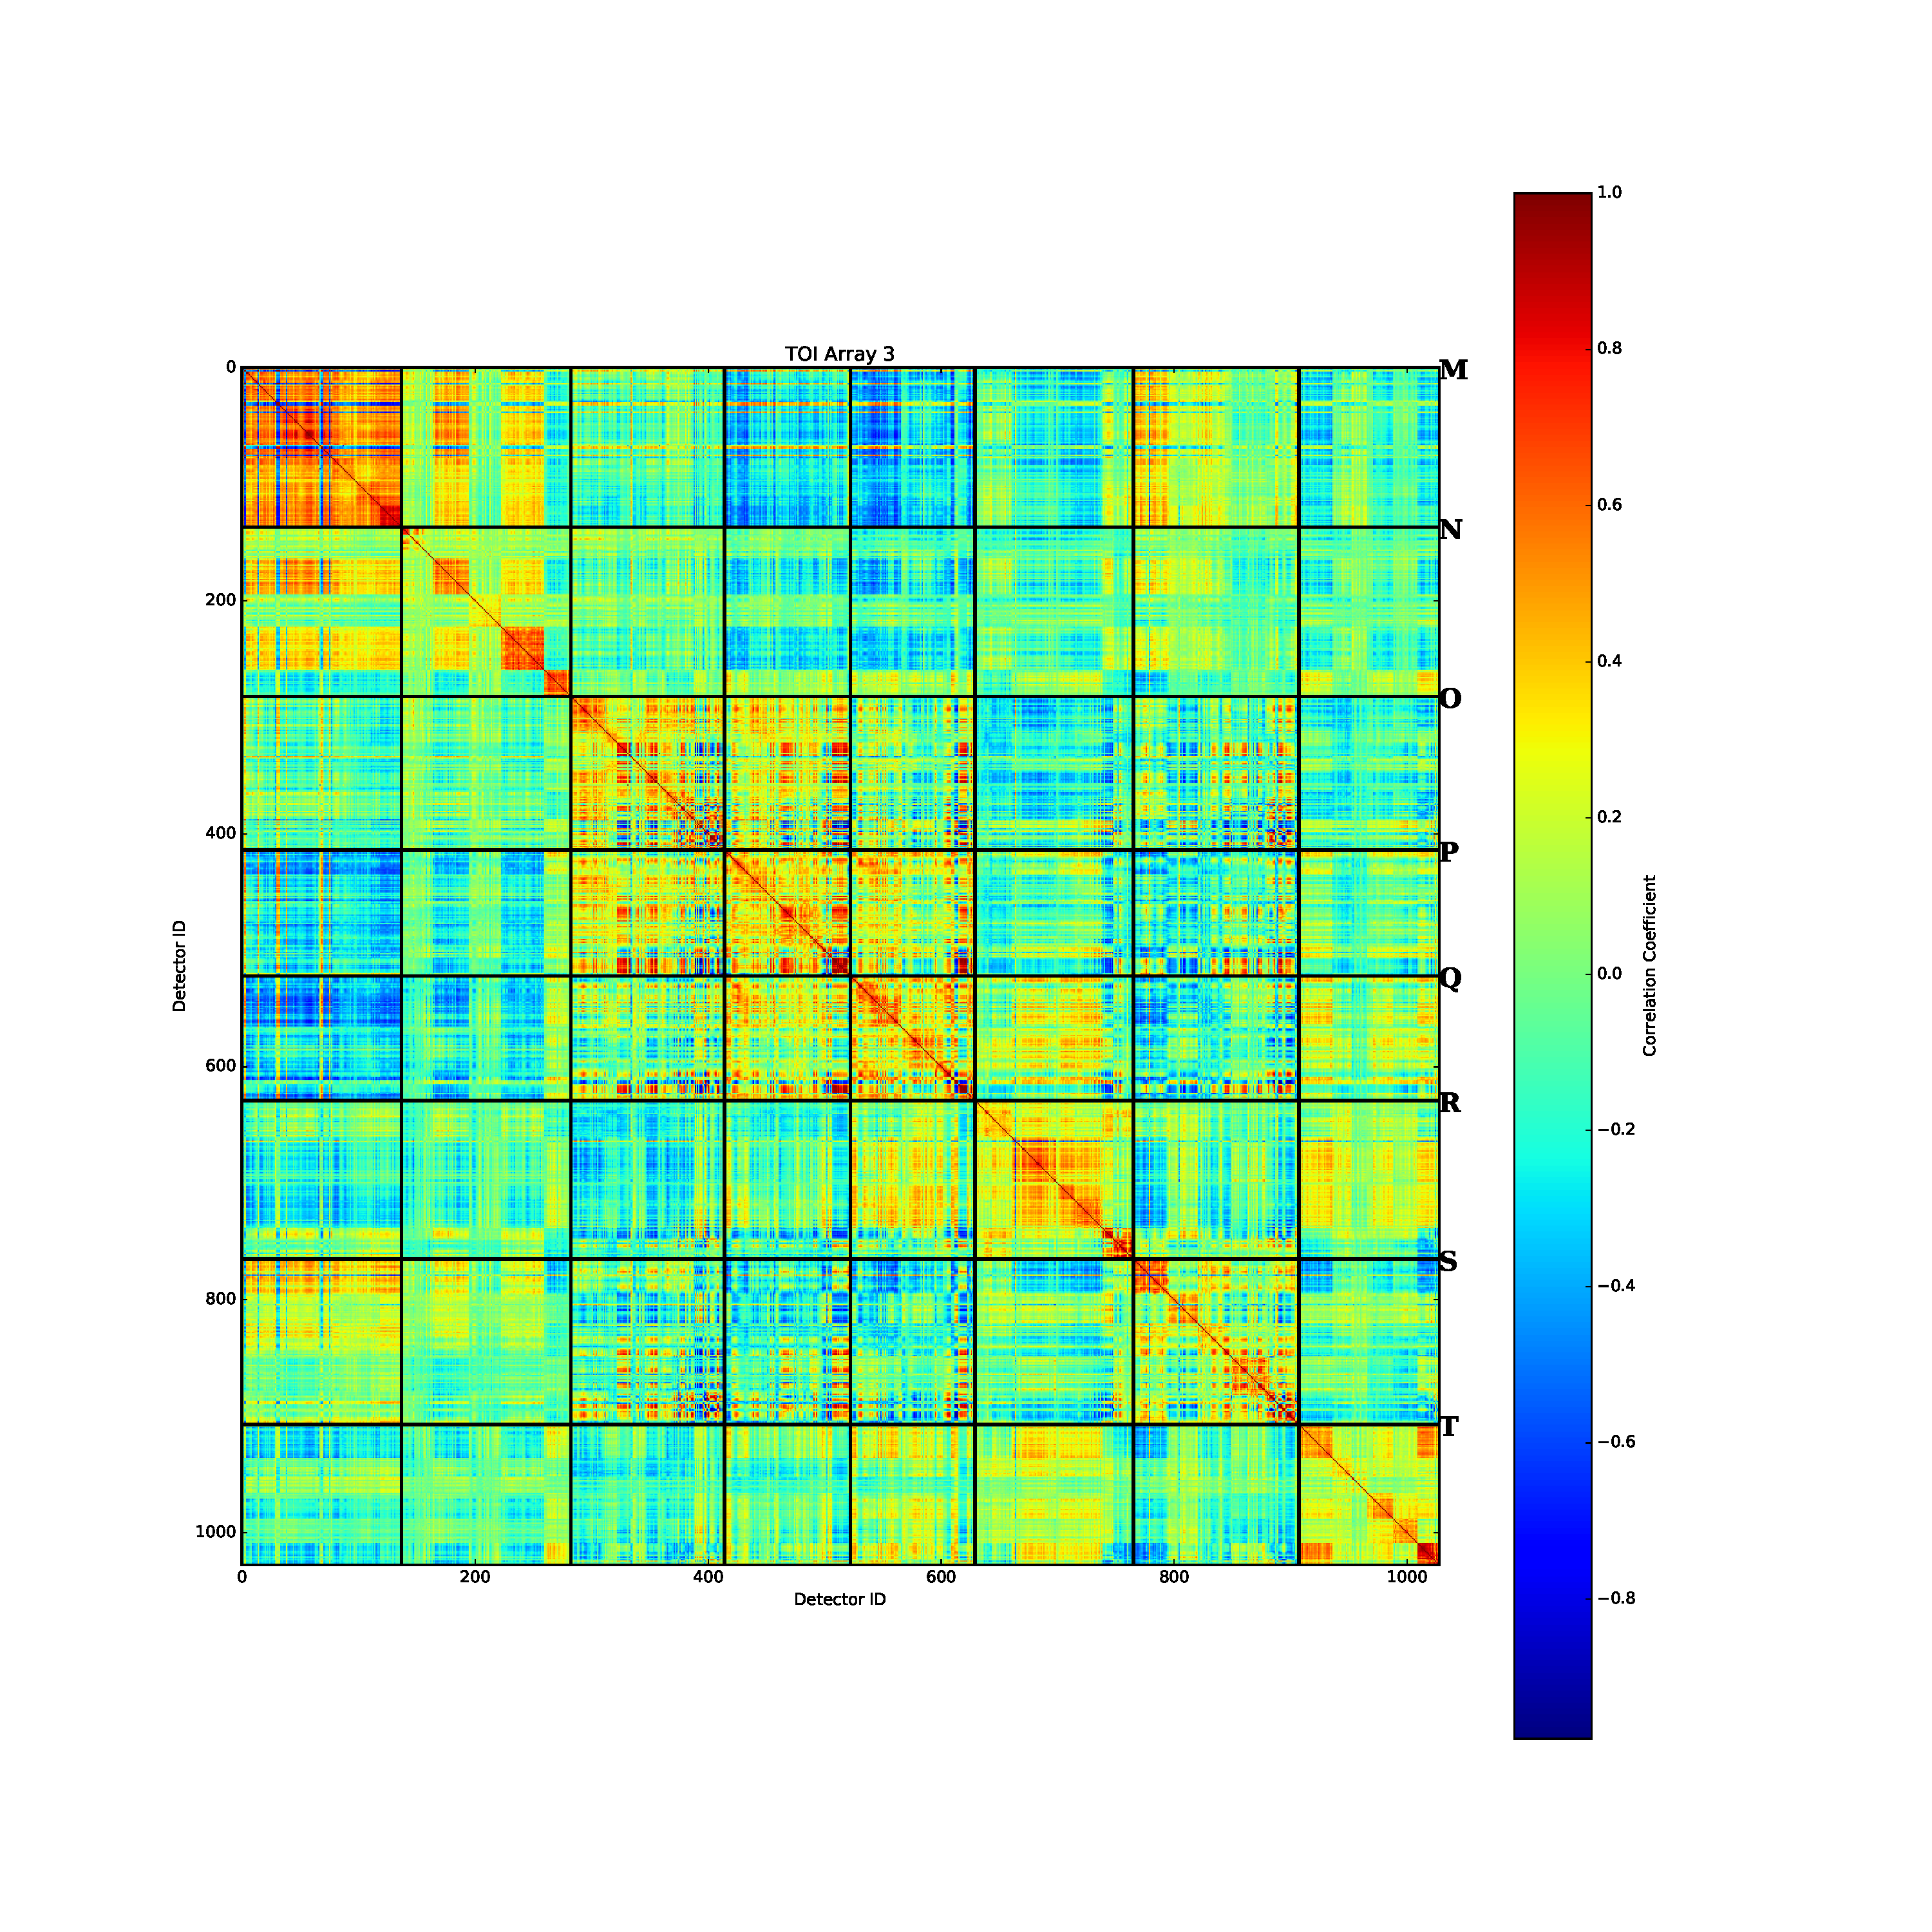
\includegraphics[width=0.3\textwidth]{Figures/DarkTests/corrmat_TOI_CM_array_3_20161213s72.pdf}
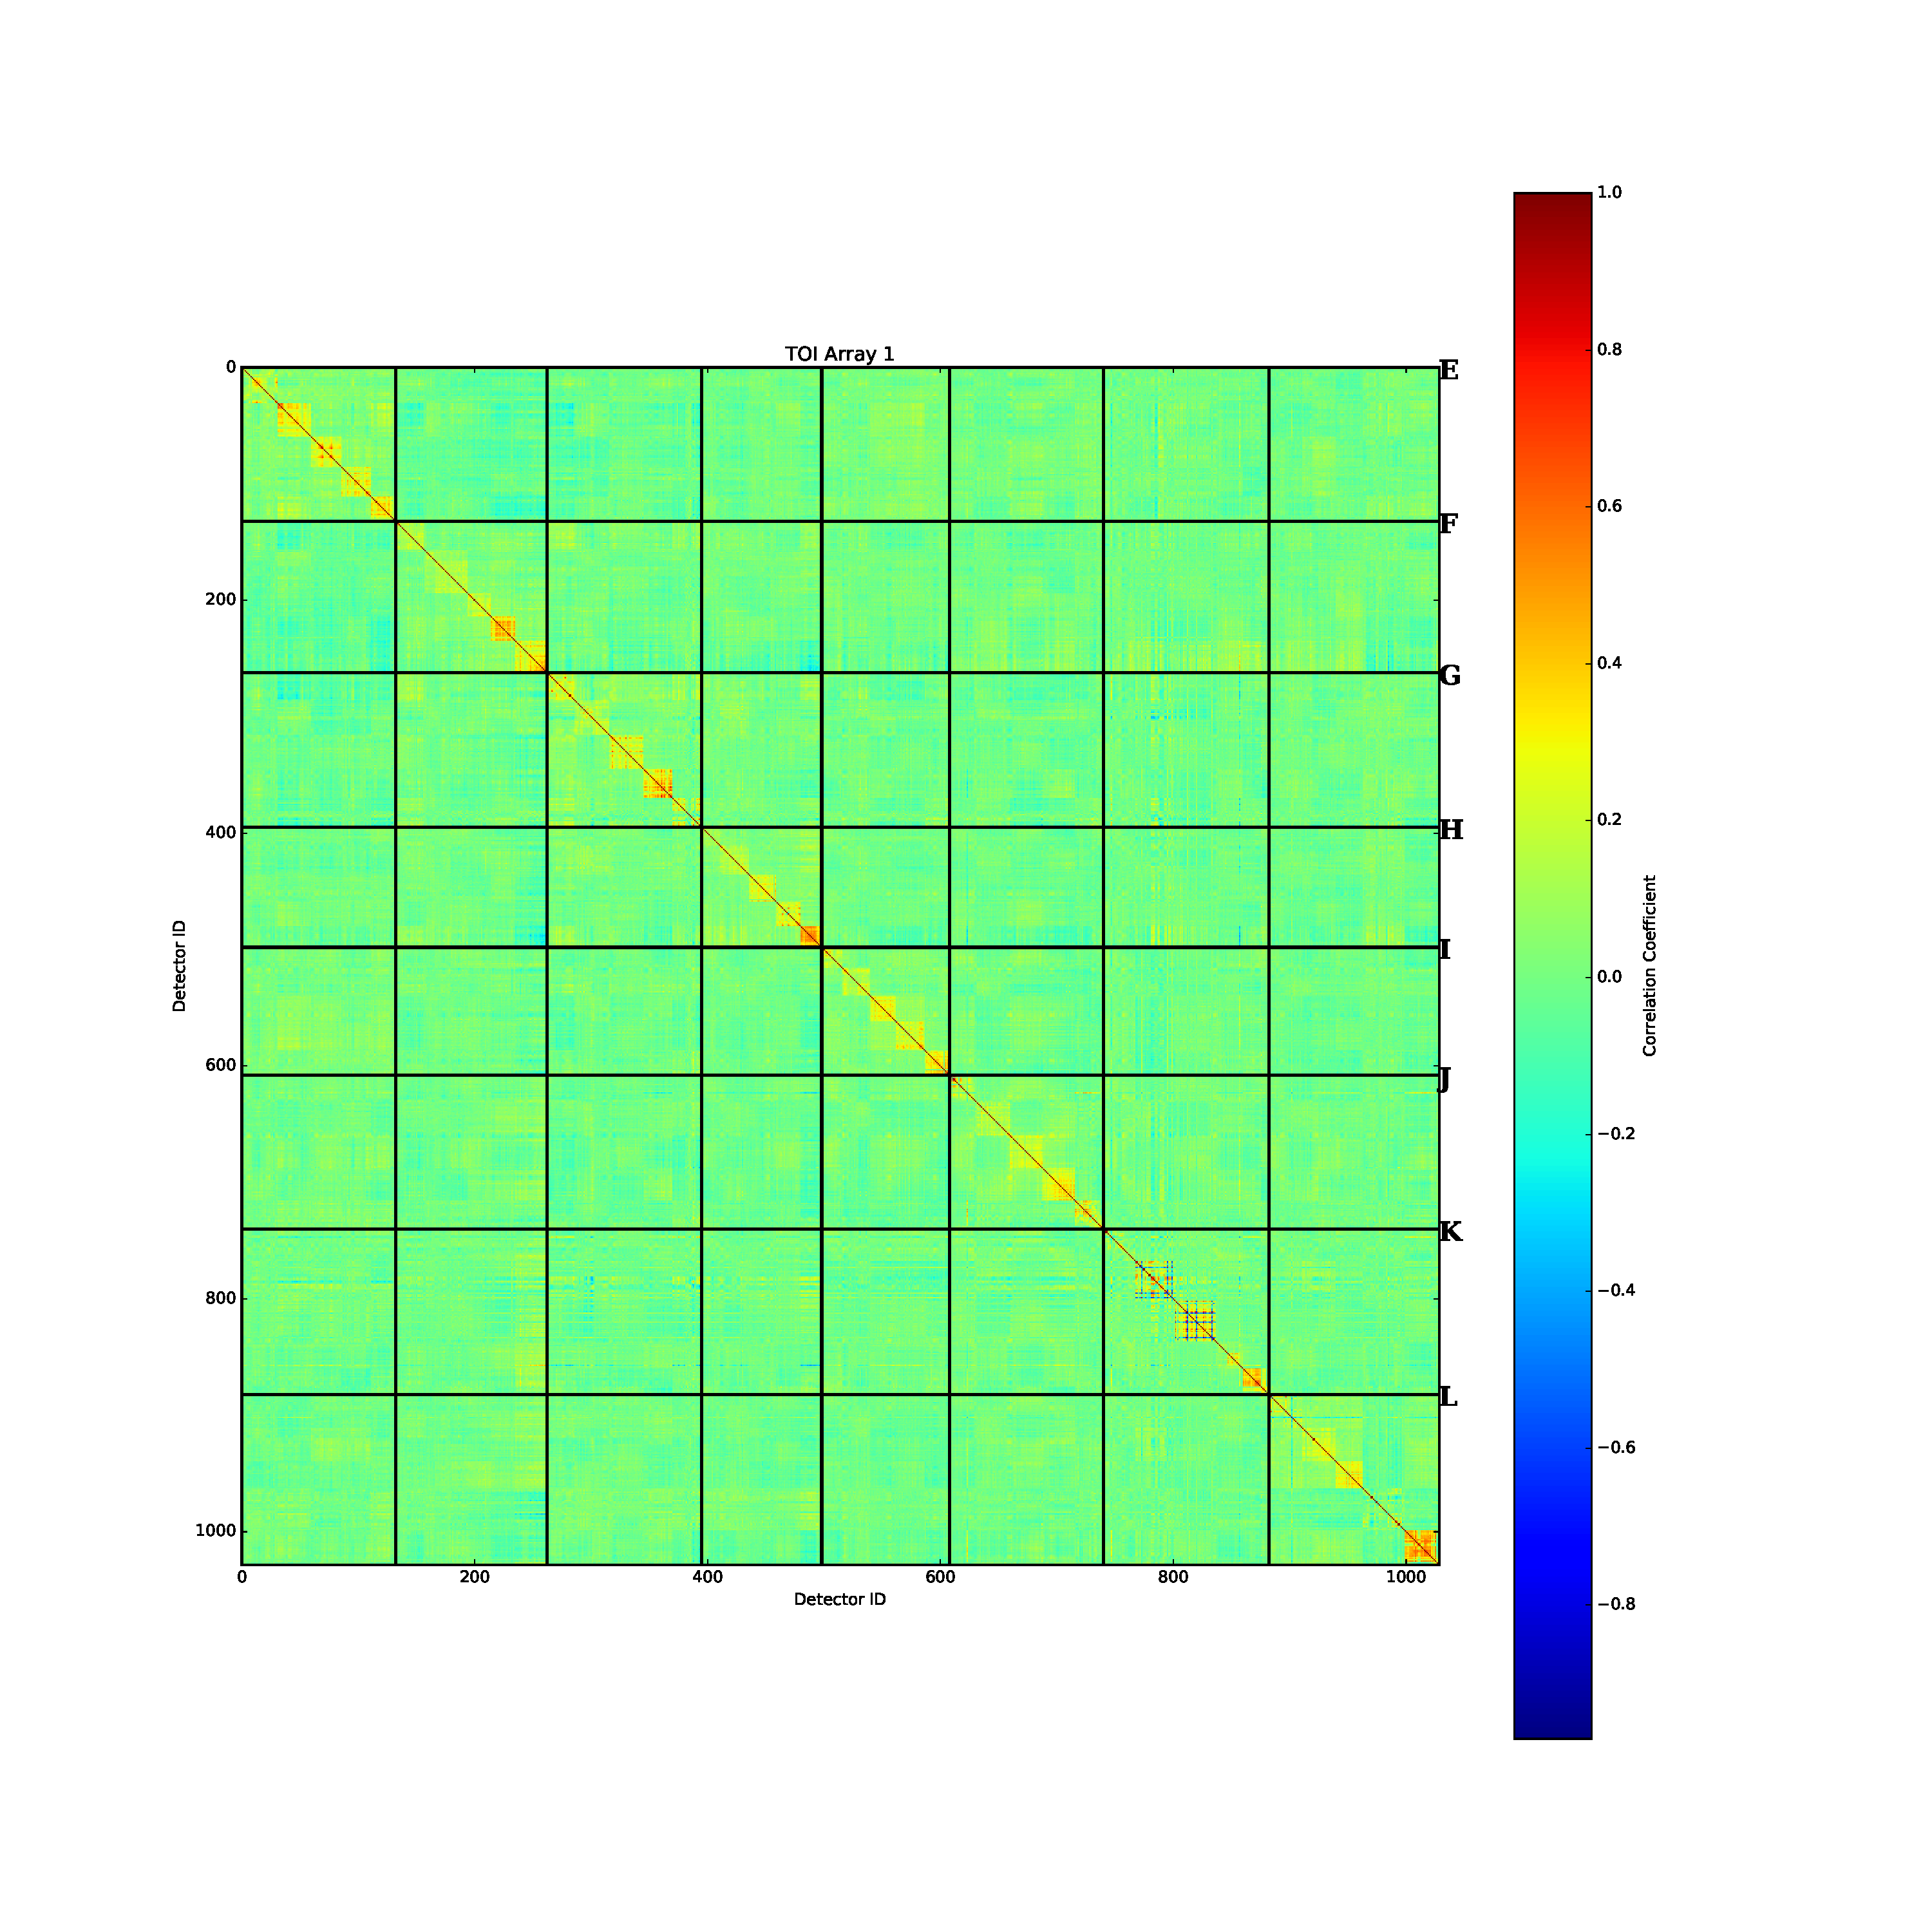
\includegraphics[width=0.3\textwidth]{Figures/DarkTests/corrmat_TOI_PCA_array_1_20161213s72.pdf}
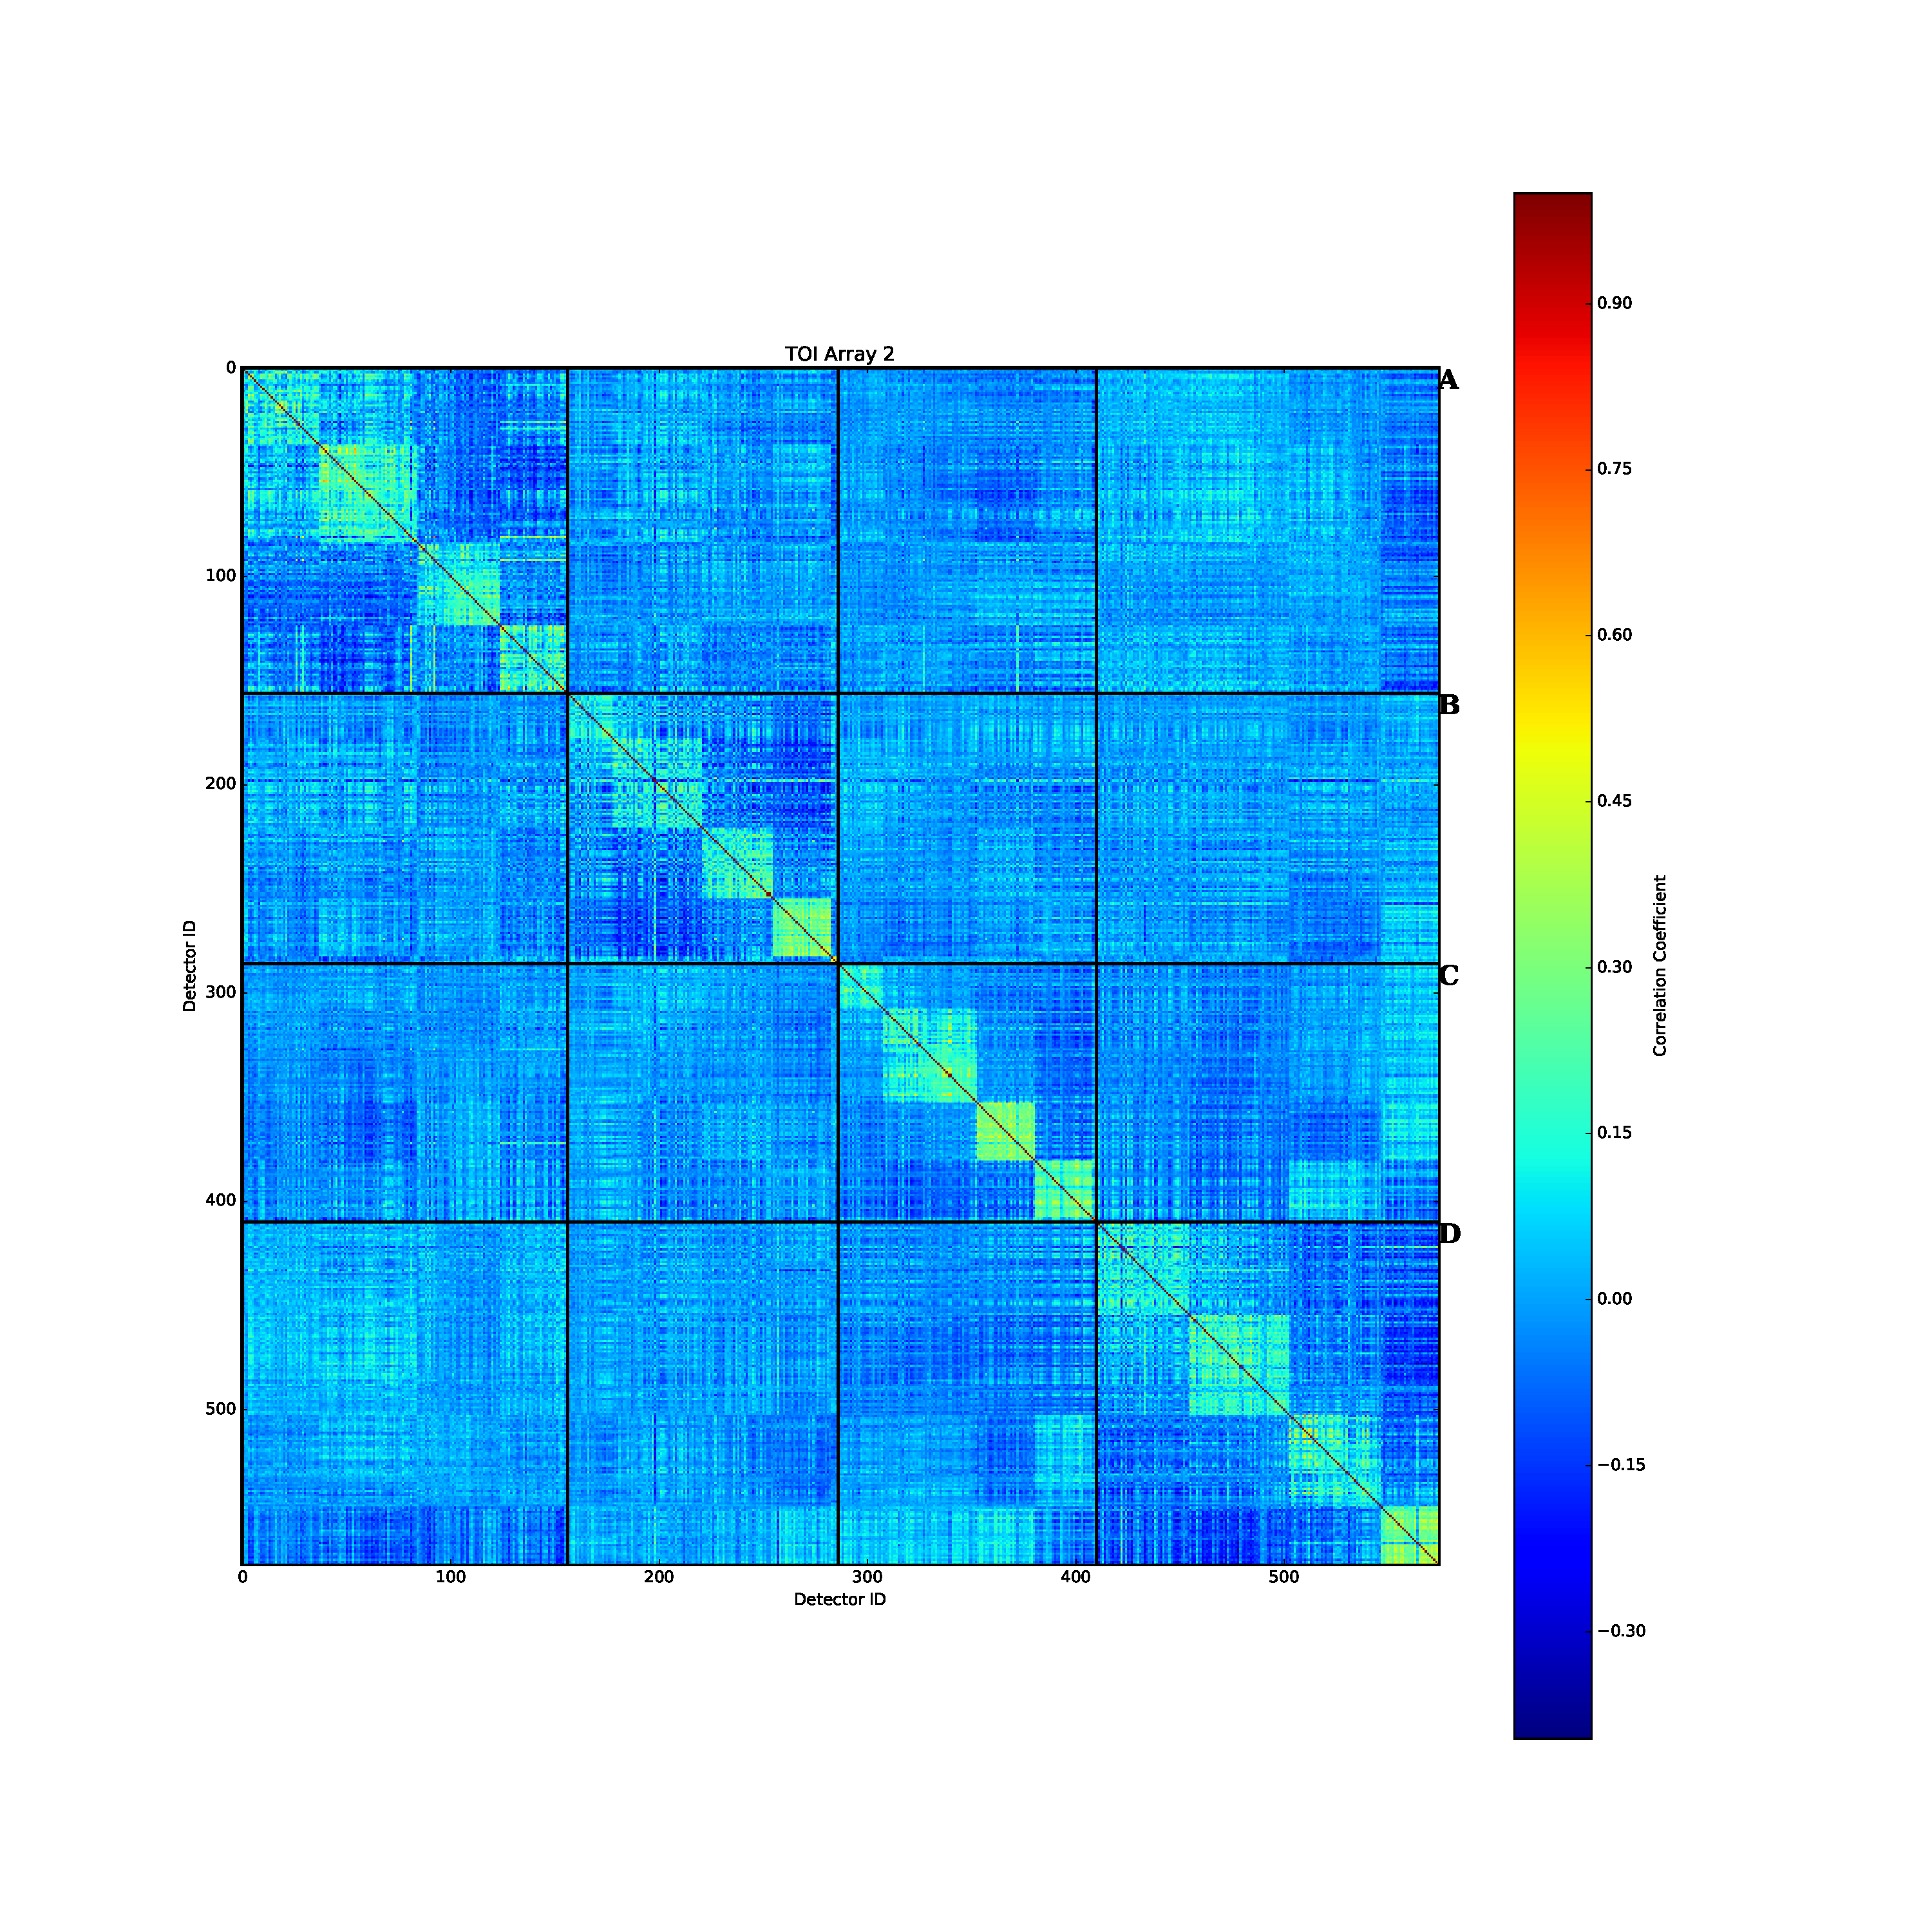
\includegraphics[width=0.3\textwidth]{Figures/DarkTests/corrmat_TOI_PCA_array_2_20161213s72.pdf}
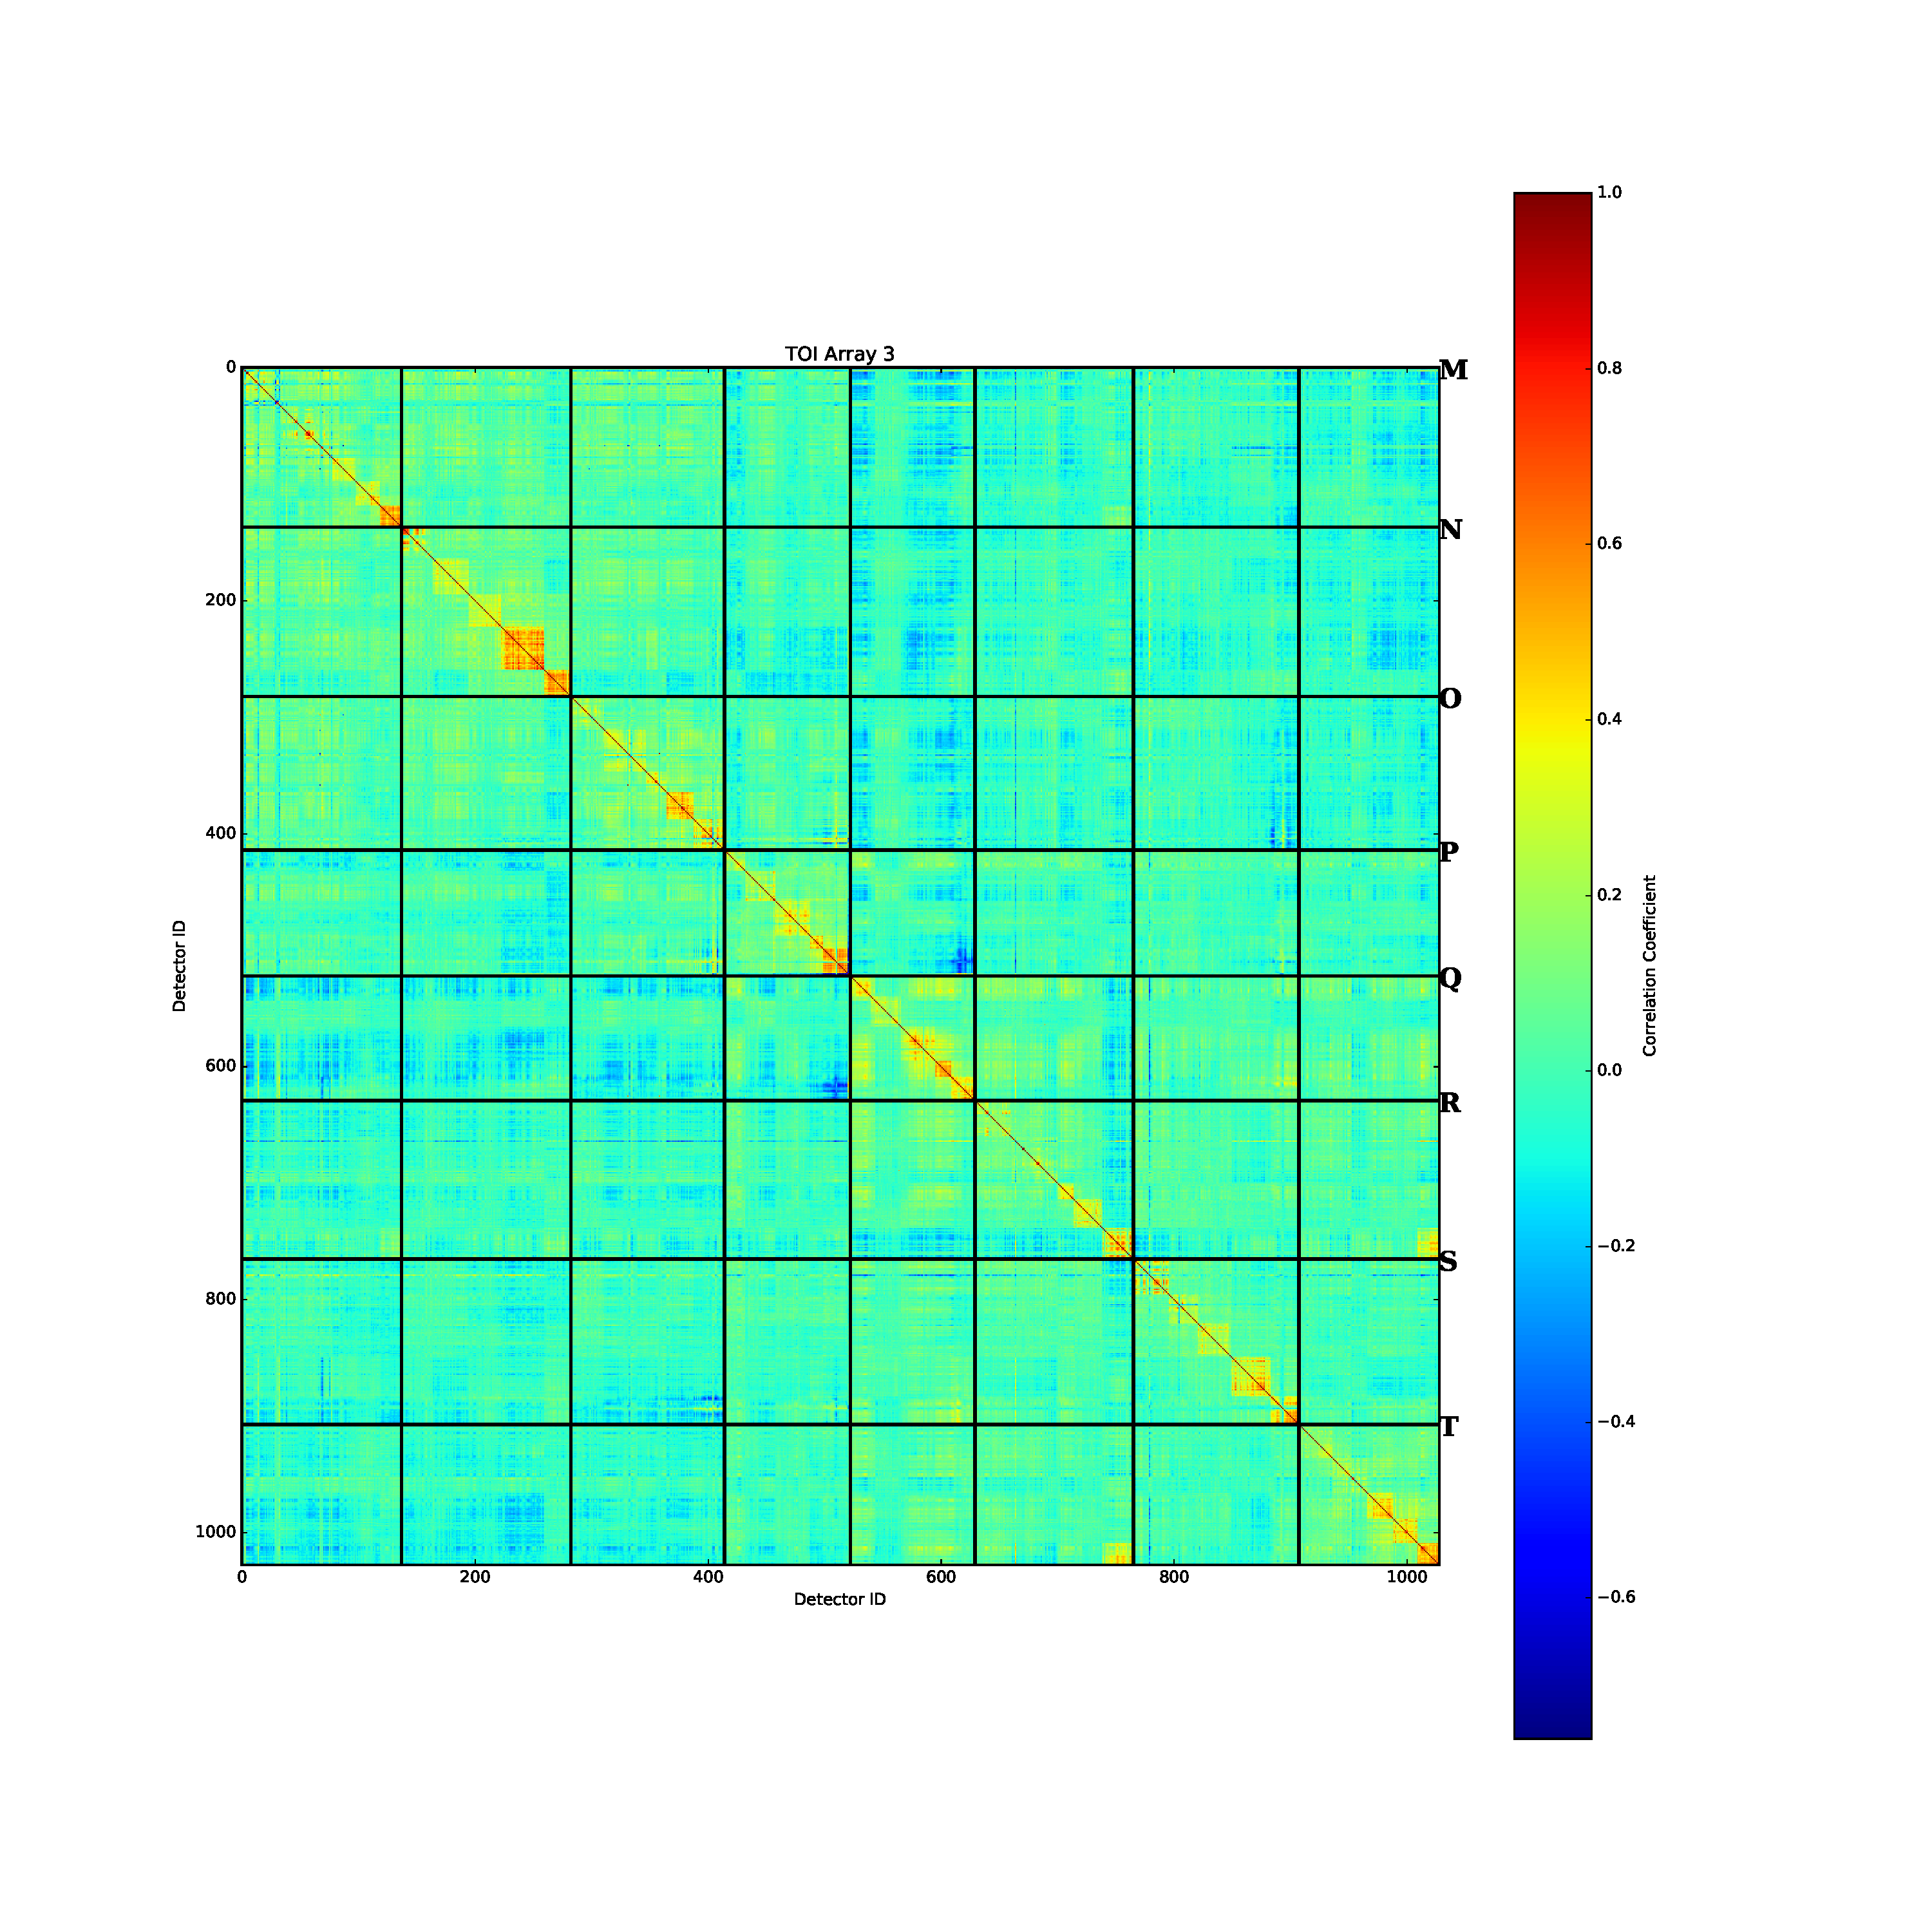
\includegraphics[width=0.3\textwidth]{Figures/DarkTests/corrmat_TOI_PCA_array_3_20161213s72.pdf}
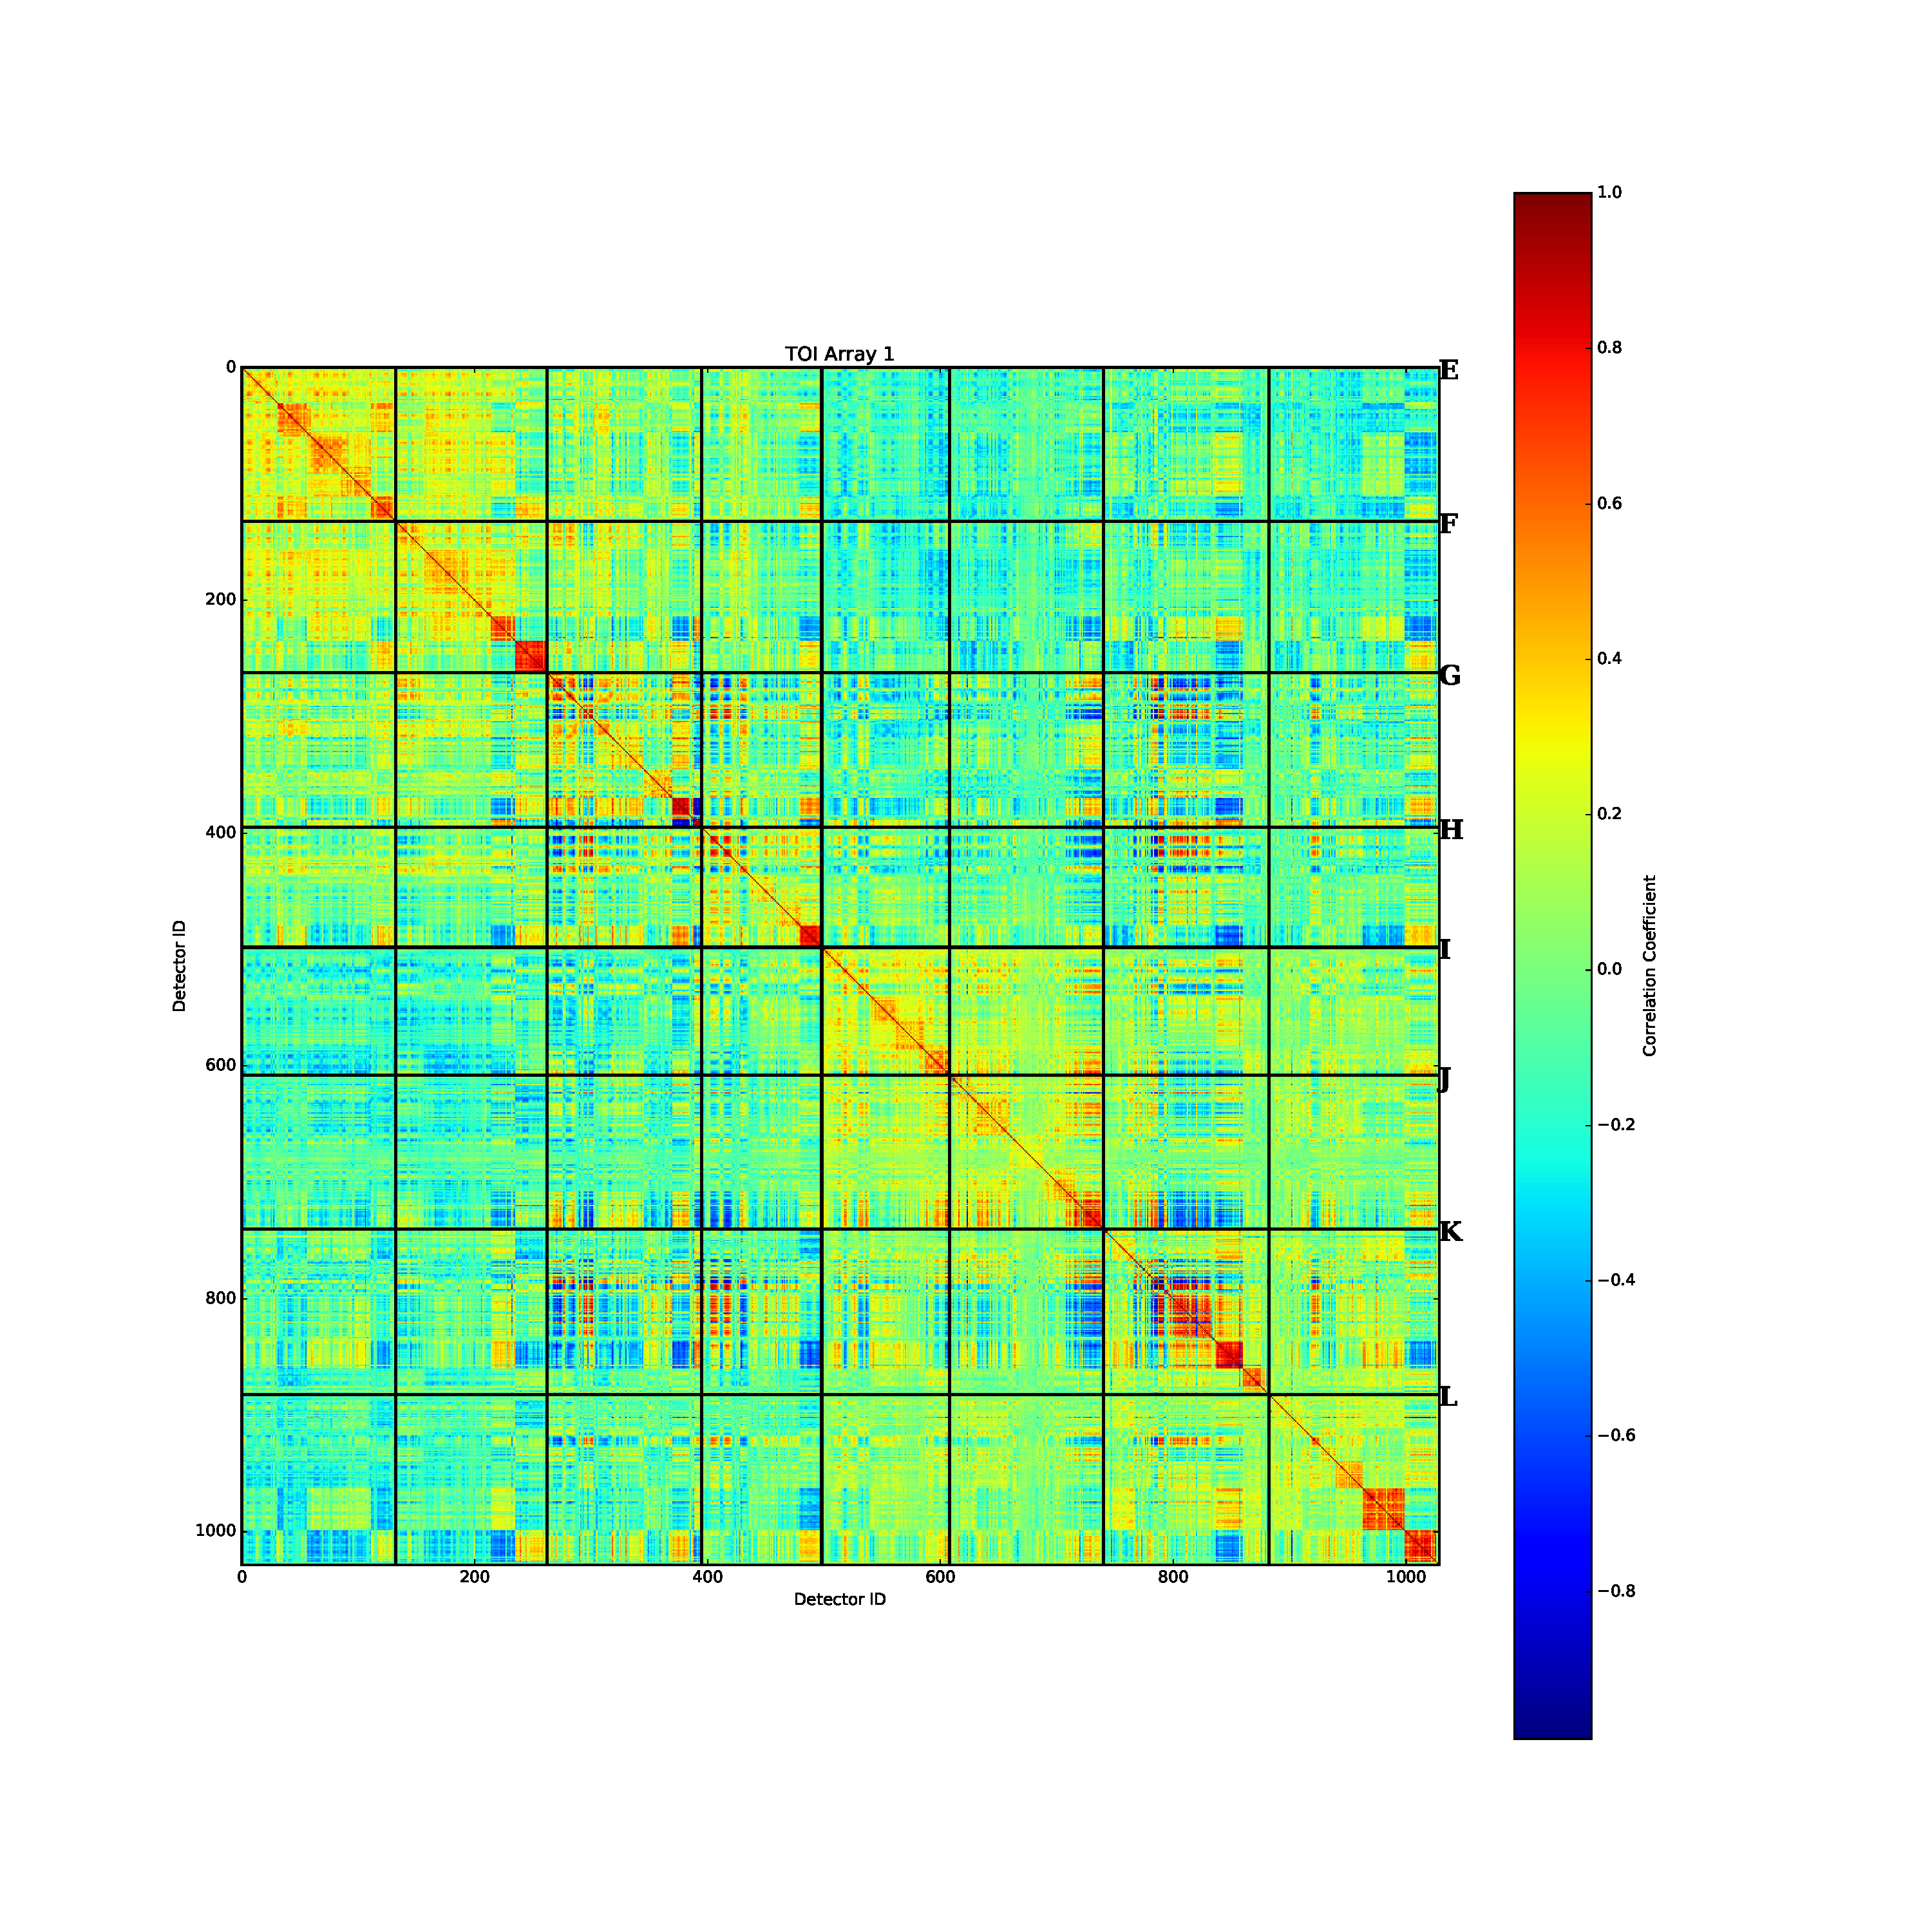
\includegraphics[width=0.3\textwidth]{Figures/DarkTests/corrmat_TOI_BC_array_1_20161213s72.pdf}
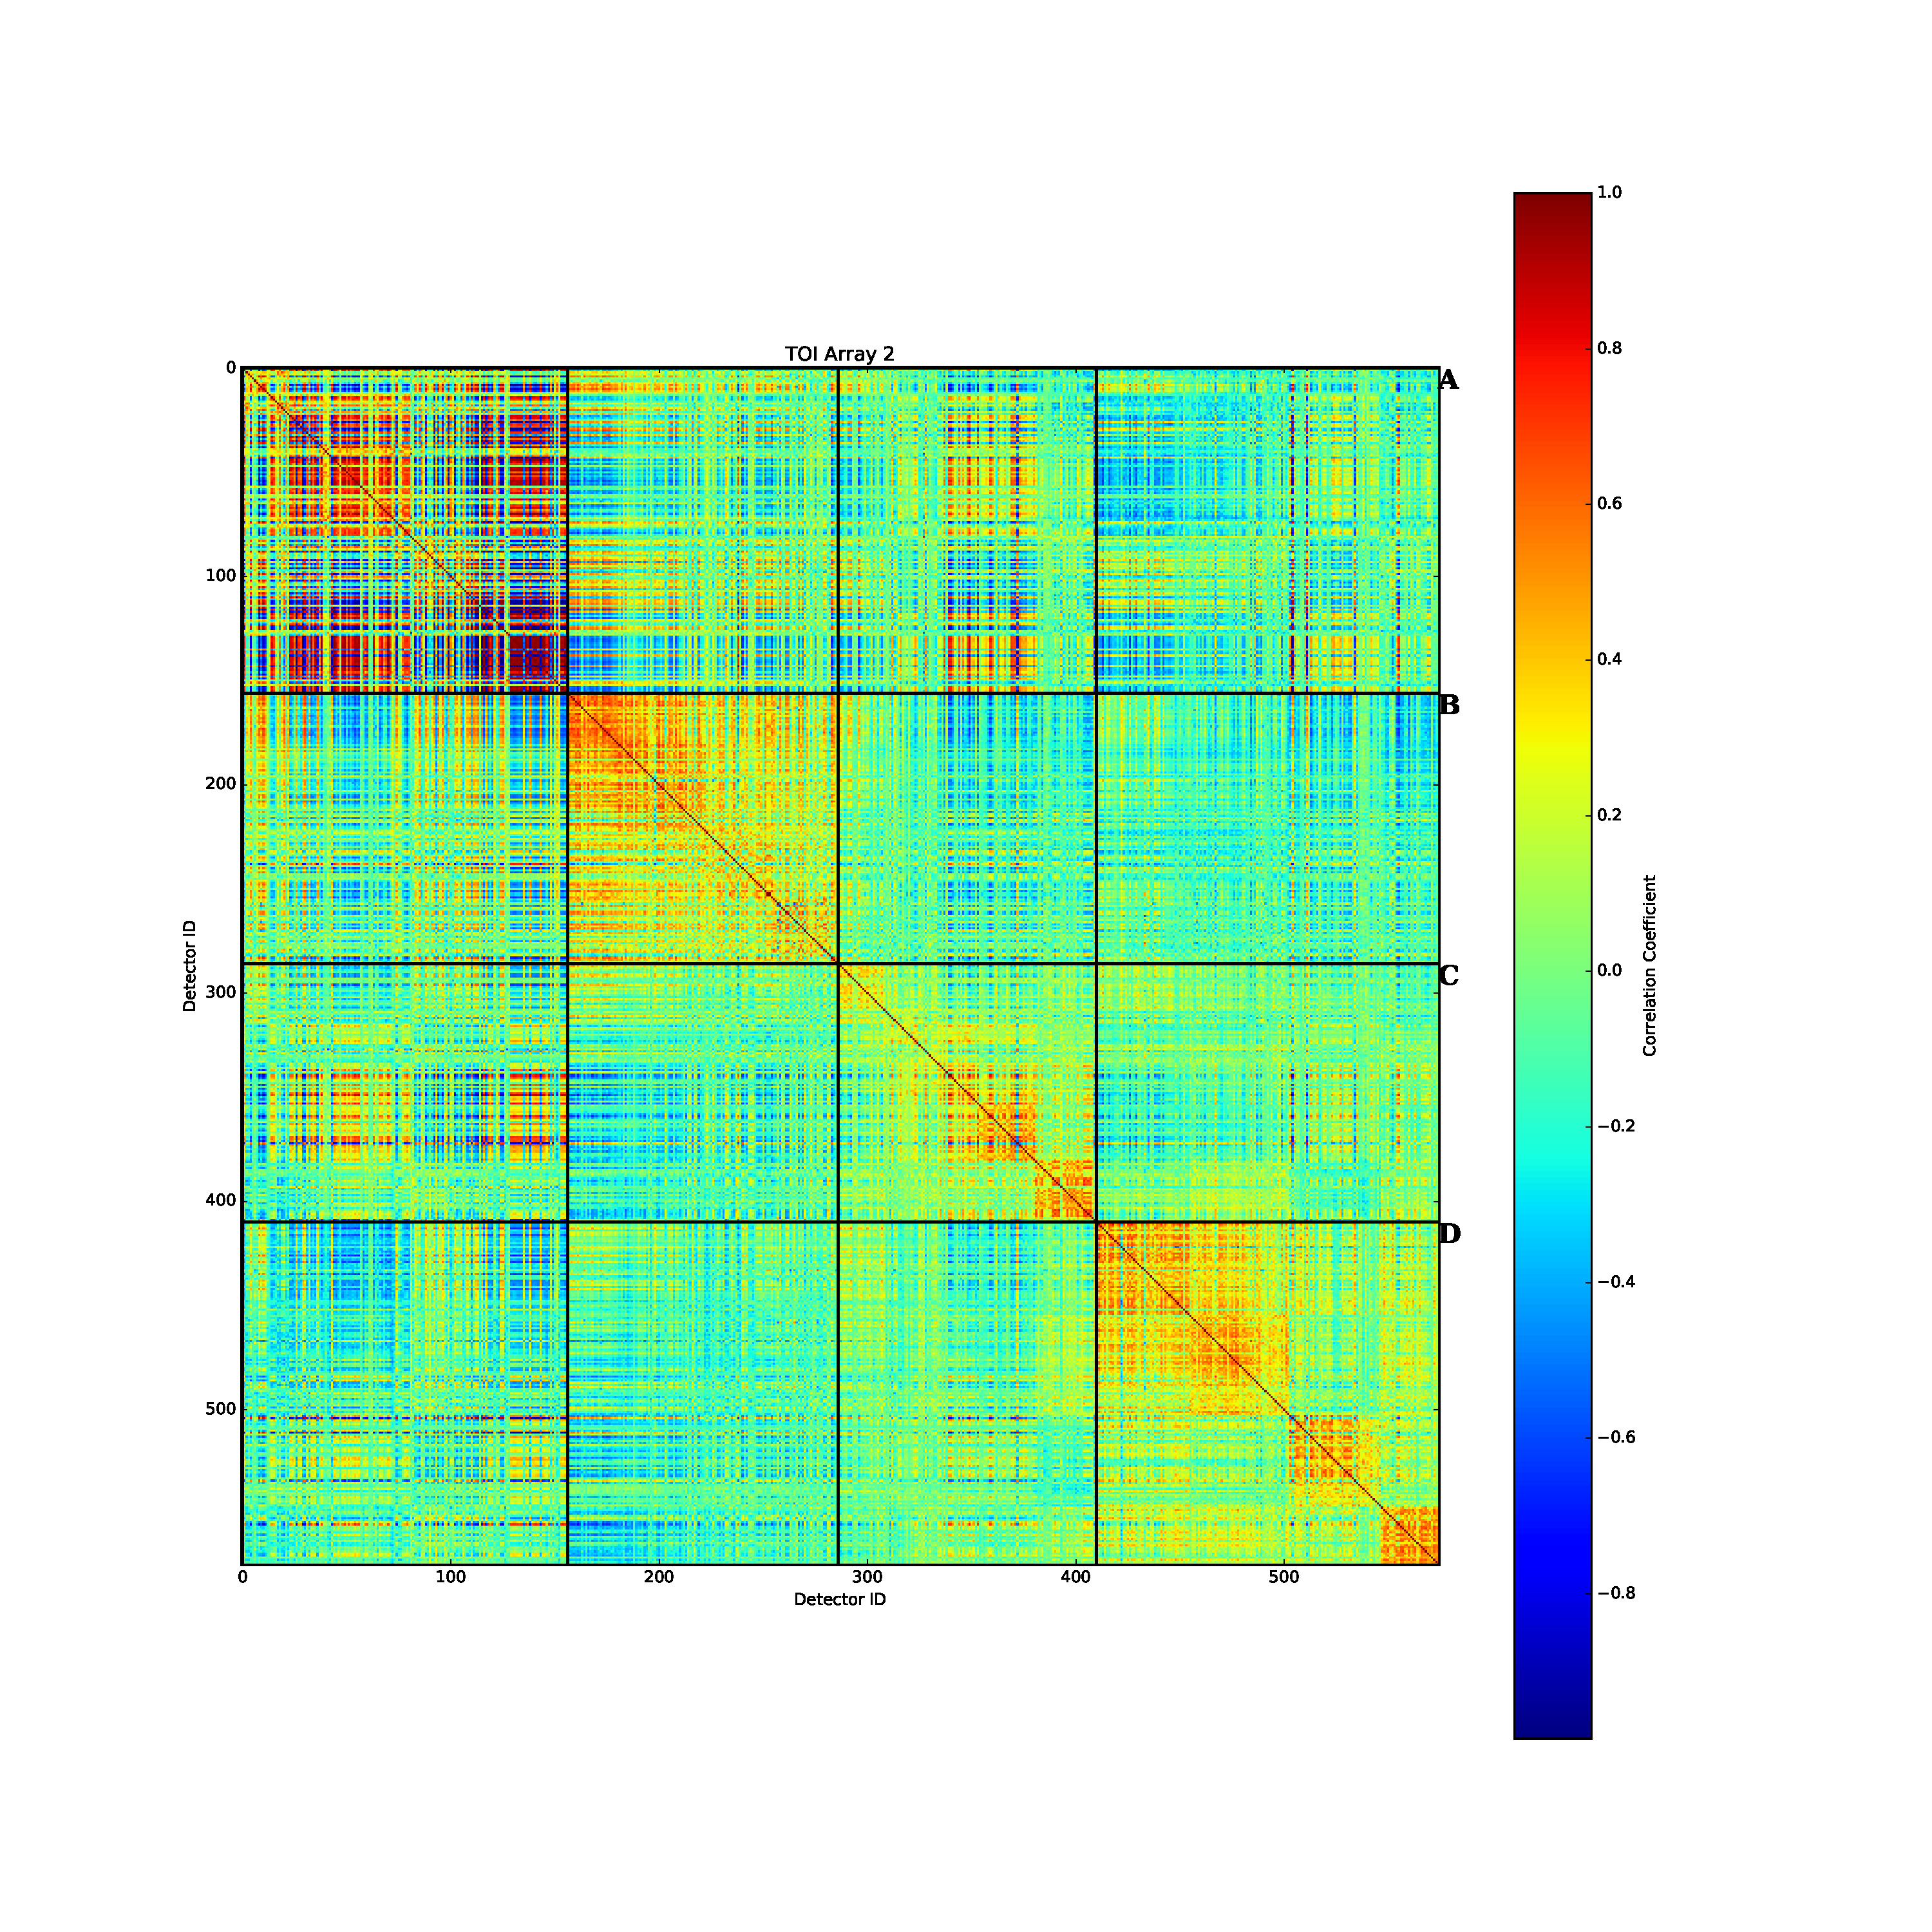
\includegraphics[width=0.3\textwidth]{Figures/DarkTests/corrmat_TOI_BC_array_2_20161213s72.pdf}
\includegraphics[width=0.3\textwidth]{Figures/DarkTests/corrmat_TOI_BC_array_3_20161213s72.pdf}
\end{center}
\caption{From left to right correlation matrices for the three NIKA2 arrays (A1, A2, and A3) for scan 20161213s72. From top to bottom we present the correlation of the raw data, after CM, PCA and BC decorrelations. \label{corrs72}}
\end{figure}


\begin{figure}[ht] % Inline image example
\begin{center}
\includegraphics[width=0.3\textwidth]{Figures/DarkTests/corrmat_TOI_array_1_20160504s97.pdf}
\includegraphics[width=0.3\textwidth]{Figures/DarkTests/corrmat_TOI_array_2_20160504s97.pdf}
\includegraphics[width=0.3\textwidth]{Figures/DarkTests/corrmat_TOI_array_3_20160504s97.pdf}
\includegraphics[width=0.3\textwidth]{Figures/DarkTests/corrmat_TOI_CM_array_1_20160504s97.pdf}
\includegraphics[width=0.3\textwidth]{Figures/DarkTests/corrmat_TOI_CM_array_2_20160504s97.pdf}
\includegraphics[width=0.3\textwidth]{Figures/DarkTests/corrmat_TOI_CM_array_3_20160504s97.pdf}
\includegraphics[width=0.3\textwidth]{Figures/DarkTests/corrmat_TOI_PCA_array_1_20160504s97.pdf}
\includegraphics[width=0.3\textwidth]{Figures/DarkTests/corrmat_TOI_PCA_array_2_20160504s97.pdf}
\includegraphics[width=0.3\textwidth]{Figures/DarkTests/corrmat_TOI_PCA_array_3_20160504s97.pdf}
\includegraphics[width=0.3\textwidth]{Figures/DarkTests/corrmat_TOI_BC_array_1_20160504s97.pdf}
\includegraphics[width=0.3\textwidth]{Figures/DarkTests/corrmat_TOI_BC_array_2_20160504s97.pdf}
\includegraphics[width=0.3\textwidth]{Figures/DarkTests/corrmat_TOI_BC_array_3_20160504s97.pdf}
\end{center}
\caption{From left to right correlation matrices for the three NIKA2 arrays (A1, A2, and A3) for scan 20160504s97. From top to bottom we present the correlation of the raw data, after CM, PCA and BC decorrelations. \label{corrs97}}
\end{figure}


\begin{figure}[ht] % Inline image example
\begin{center}
\includegraphics[width=0.3\textwidth]{Figures/DarkTests/corrmat_TOI_array_1_20160313s87.pdf}
\includegraphics[width=0.3\textwidth]{Figures/DarkTests/corrmat_TOI_array_2_20160313s87.pdf}
\includegraphics[width=0.3\textwidth]{Figures/DarkTests/corrmat_TOI_array_3_20160313s87.pdf}
\includegraphics[width=0.3\textwidth]{Figures/DarkTests/corrmat_TOI_CM_array_1_20160313s87.pdf}
\includegraphics[width=0.3\textwidth]{Figures/DarkTests/corrmat_TOI_CM_array_2_20160313s87.pdf}
\includegraphics[width=0.3\textwidth]{Figures/DarkTests/corrmat_TOI_CM_array_3_20160313s87.pdf}
\includegraphics[width=0.3\textwidth]{Figures/DarkTests/corrmat_TOI_PCA_array_1_20160313s87.pdf}
\includegraphics[width=0.3\textwidth]{Figures/DarkTests/corrmat_TOI_PCA_array_2_20160313s87.pdf}
\includegraphics[width=0.3\textwidth]{Figures/DarkTests/corrmat_TOI_PCA_array_3_20160313s87.pdf}
\includegraphics[width=0.3\textwidth]{Figures/DarkTests/corrmat_TOI_BC_array_1_20160313s87.pdf}
\includegraphics[width=0.3\textwidth]{Figures/DarkTests/corrmat_TOI_BC_array_2_20160313s87.pdf}
\includegraphics[width=0.3\textwidth]{Figures/DarkTests/corrmat_TOI_BC_array_3_20160313s87.pdf}
\end{center}
\caption{From left to right correlation matrices for the three NIKA2 arrays (A1, A2, and A3) for scan 20160313s87. From top to bottom we present the correlation of the raw data, after CM, PCA and BC decorrelations. \label{corrs87}}
\end{figure}


\subsection{RMS of the noise}

We present in Figure~\ref{rms299} the rms, in Hz, of the raw (dark blue) and decorrelated (CM, blue; PCA, red; and BC, cyan),data for the N2R7 dark test scan 21612101s299. We also show for comparison the rms of the data by extrapolating the median high frequency noise (PS, violet).
For the three arrays we observe that decorrelation reduces significantly the rms noise. The most efficient method is PCA as one would expect from previous results in the noise correlation matrix. \\

For each array the detectors are ordered by electronic box (separated by vertical black lines in the figure) and within each electronic box by increasing resonant frequency. We observe that median high frequency noise increases with increasing resonant frequency. A similar effect is observed for the PCA and BC rms noise but for some pathological detectors or electronic boxes. While in A2 the rms noise increases monotoneously with resonant frequency in arrays A1 and A3 we observe also observe fine structure within eash electronic box. For array A2, electronic box A, shows significantly larger raw rms. For array A1 box K seems to have a larger number of anomalous detectors than the other boxes. In array A3 all boxes seem to be equivalent to first order. Both in A1 and A3 we find complex structure within each box, which are not present in A2. \\

Similar results are found for scan 20161213s72 as shown in Figure~\ref{rms72}. However, we stress that the atmospheric emission shows significant contribution at high frequency (see PS) that is significantly reduced after decorrelation. \\

We have also computed the noise rms for the scans of N2R4 20160504s97 and 20160313s87. For arrays A1 and A3 the results are very similar to those for the N2R7 scans. However, we clearly observe that A2 is significantly worse in terms of misbehaving pixels.


%------------------------------------------------
\begin{figure}[ht] % Inline image example
\begin{center}
\includegraphics[scale=0.26]{Figures/DarkTests/rms_TOI_array_1_20161211s299.pdf} 
\includegraphics[scale=0.26]{Figures/DarkTests/rms_TOI_array_2_20161211s299.pdf} 
\includegraphics[scale=0.26]{Figures/DarkTests/rms_TOI_array_3_20161211s299.pdf} 
\end{center}
\caption{RMS noise for arrays 1,2,and 3 (top to bottom) for scan 20161211s299. The rms is computed for the raw data, and for the three decorrelation methods, CM. PCA and BC. The rms value for the level of white is also computed from the raw data power spectrum (PS). \label{rms299}}
\end{figure}


\begin{figure}[ht] % Inline image example
\begin{center}
\includegraphics[scale=0.26]{Figures/DarkTests/rms_TOI_array_1_20161213s72.pdf} 
\includegraphics[scale=0.26]{Figures/DarkTests/rms_TOI_array_2_20161213s72.pdf} 
\includegraphics[scale=0.26]{Figures/DarkTests/rms_TOI_array_3_20161213s72.pdf} 
\end{center}
\caption{Same as Figure~\ref{rms299} but for scan 20161213s72. \label{rms72}}
\end{figure}

\begin{figure}[ht] % Inline image example
\begin{center}
\includegraphics[scale=0.26]{Figures/DarkTests/rms_TOI_array_1_20160504s97.pdf} 
\includegraphics[scale=0.26]{Figures/DarkTests/rms_TOI_array_2_20160504s97.pdf} 
\includegraphics[scale=0.26]{Figures/DarkTests/rms_TOI_array_3_20160504s97.pdf} 
\end{center}
\caption{Same as Figure~\ref{rms299} but for scan 20160504s97. \label{rms97}}
\end{figure}



\begin{figure}[ht] % Inline image example
\begin{center}
\includegraphics[scale=0.26]{Figures/DarkTests/rms_TOI_array_1_20160313s87.pdf} 
\includegraphics[scale=0.26]{Figures/DarkTests/rms_TOI_array_2_20160313s87.pdf} 
\includegraphics[scale=0.26]{Figures/DarkTests/rms_TOI_array_3_20160313s87.pdf} 
\end{center}
\caption{Same as Figure~\ref{rms299} but for scan 20160313s87. \label{rms87}}
\end{figure}



\subsection{Discussion}

Using dark test measurements we have identified several noise components that require using complex decorrelation methods. Event in the case of multiple template decorrelation we find residual correlation between detectors that seems to be related to electronic subbands. Similar results are found when analyzing faint source scans. We find significant differences between N2R4 and N2R7 scans. \\

After decorralation using multiple template procedures we reduce significantly the rms of the noise. In the case of dark test it becomes of the level of the high frequency noise. For faint source scans we also diminish the high frequency noise, which is probably dominated by atmospheric emission. We find significant differences between the noise levels in A1 and A3, which might be explained by gain differences (to be verified). For some electronic boxes in A2 the rms noise is significantly larger than for the others. For the three arrays we find increasing noise with increasing resonant frequency withing each electronic box.This is probably related to the difference of gains between subbands in the electronics. Furthermore, we find in A1 and A3 extra low frequency structures in the rms which are not identified yet.



%----------------------------------------------------------------------------------------
%	SENSITIVITIES
%----------------------------------------------------------------------------------------
\section{Sensitivities}
\label{se:nefd}
%%
%%
%%      SECTION: SENSITIVITY
%%

\begin{figure}
\begin{center}
%\includegraphics[clip, angle=0, scale =
%  0.5]{Figures/NEFD_HLS091828_20170226s415_FXDC0C1_GaussPhot.png}
\includegraphics[clip, angle=0, scale = 0.5]{Figures/nefd_mpfit_HLS091828.eps}
\caption{Kids Xcalib with fixed fwhm 12.5 and 18.5, \hls.}
\label{fig:nefd_vs_t}
\end{center}
\end{figure}

{\bf The specs/goals ``NEFD on X \% of pixels'' should be understood as : we have
XX\% valid pixels, and with these pixels, we have an NEFD of YY. We should not
discard some fraction of our pixels and estimate an NEFD on this subset.}\\

\hls is moderately faint source, expected to be below 100~mJy at 1mm and
XX~mJy at 2mm {\bf check values in NIKA1 paper + use SED for predictions in
  NIKA2's bands}. This source was chosen for its flux and its availability during
Run9 for long integration. It has been observed for XX hours in total over three
nights.


\subsection{Observations}

As part of the NIKA2 Science Verification that took place in February 2017, we
observed an area of 185~arcmin$^2$, centered on \hls, (a lensed dusty galaxy at
z=5.24 \cite{combes2012}) during about 9~hours. The scans were 8x5~arcmin$^2$,
alternatively oriented in (ra,dec), (dec,ra), (az,el), (el,az). This leads to
the coverage presented on Fig.~\ref{fig:hls_cov} and effective integration times
on \hls\ of $\sim 2.4$\,hours at 2\,mm and $\sim 1.7$\,hours at 1.2\,mm (the
difference comes from the different density of detectors across the field of
view for the two bands). This allowed us to reach $1\sigma$ sensitivities of
about 0.3~mJy at 1.2\,mm and 0.1~mJy at 2\,mm on \hls. The integration time in a
map pixel $t_p$ of size $r\times r$~arcsec$^2$ is given by the number of hits in
this pixel $N_p$, divided by the sampling frequency $\nu$. This estimate is not
the time $t_{obs}$ that enters the definition of the NEFD and which is the time
spent by the matrix ``overall'' on the region where we give the
sensitivity. Indeed, we must account for the density of KIDs in the focal plane
compared to the map resolution : assume there are two KIDs per map pixel, then
$t_p = 2 t_{obs}$. A contrario, if the KIDs are sparsely distributed accross the
focal plane, some map pixels are empty while they are physically covered by the
FOV. Let's call $g$ the spacing between KIDs in arcsec in the FOV, we thus have:

\begin{eqnarray}
t_{obs} &=& \frac{t_p}{N_{kids\,per\,pix}} \nonumber\\
&=& \frac{t_p}{N_{kids}/N_{pix}} \nonumber\\
&=& \frac{t_p\pi R_{FOV}^2/r^2}{\pi R_{FOV}^2/g^2} \nonumber\\
&=&t_p g^2r^2
\end{eqnarray}

\begin{figure}[htbp]
\begin{center}
\includegraphics[clip, angle=0, scale = 0.30]{Figures/hls_sensit_1mm.eps}
\includegraphics[clip, angle=0, scale = 0.30]{Figures/hls_sensit_2mm.eps}
\caption{Sensitivity per beam in mJy at 1 and 2mm}
\label{fig:hls_cov}
\end{center}
\end{figure}


\subsection{Data processing}

The data were decorrelated using the {\tt common-monde-one-block} method
(cf.~\ref{se:cm1blck}), masking a disk of 60~arcsec radius centered \hls.  The
scans have been combined with standard inverse noise weighting. The noise in
each map pixel is derived from the rms of the background corrected by the square
root of the number of observations per pixel (N1). If the noise was perfectly
gaussian, the distribution of the map signal over this noise estimate (far from
the source) would be a normalized gaussian. In practice, this leads to gaussians
that 1.6 and 1.5 larger. We therefore increase our noise estimate (N1) by these
factors to derive our final estimates. Should the extra sources that pop up in
the field contribute to this estimate, they would only make our estimate more
conservative.

\subsection{NEFD Methods 1 and 2: deep integration}

These data can be used to derive the NEFD in several ways. One is to fit the
evolution of the uncertainty on the flux of the source $\sigma_\phi$ with the
integration time. Another one is to produce jackknife maps with the data and to
measure the uncertainty on the flux in the end, while estimating the time of
integration. Results are summarized in
Tab.~\ref{tab:nefd}. Fig.~\ref{fig:nefd_vs_t} shows the decrease of the
uncertainty on the measured flux at the center of the map as a function of
time. We either fit a power law or fix the power law to -0.5 and fit only the
amplitude. Uncertainties on these values have been estimated via a bootstrap
method: we randomize the scans and derive the standard deviation of the average
of $n$ scans for any $n$ between 1 and the total number of scans. This gives us
an estimate of the uncertainty on $\sigma_\phi$ for a time of integration
corresponding to $n$ scans. Strictly speaking, all the scans do not have the
exact same duration, but the difference is negligible here.

\begin{table}
\begin{tabular}{|l|l|l|l|l|}
\hline
Array & Free power law & Fixed power law $t^{-0.5}$ & Jackknife & Instrument \\
\hline
A1       & $47.9$ mJy.s$^{-0.54}$ & $37.9$ mJy.s$^{1/2}$ & 35.6 mJy.s$^{1/2}$ & $33.3$ (5) mJy.s$^{1/2}$\\
A2       & $5.2$  mJy.s$^{-0.51}$ & $4.8$  mJy.s$^{1/2}$ & 5.7  mJy.s$^{1/2}$ & $5.8$  (5) mJy.s$^{1/2}$\\
A3       & $38.9$ mJy.s$^{-0.54}$ & $30.6$ mJy.s$^{1/2}$ & 30.4 mJy.s$^{1/2}$ & $28.4$ (4) mJy.s$^{1/2}$\\
A1 \& A3 & $28.5$ mJy.s$^{-0.53}$ & $23.6$ mJy.s$^{1/2}$ & 22.4 mJy.s$^{1/2}$ & $21.1$ (3) mJy.s$^{1/2}$\\
\hline
\end{tabular}
\label{tab:nefd}
\caption{Noise integration with observation time and associated derivations of
  the NEFD. These values do not account for the extra {\color{red} \bf XXXX \%}
  uncertainty on absolute calibration.}
\end{table}
%       33.325263       5.2024647
%       28.397230       4.5723151
%       21.143376       4.1538804
%       5.7628233       3.3094792


\begin{figure}
\begin{center}
\includegraphics[clip, angle=0, scale =0.8]{Figures/NEFDIndScans/nefd_tau_run22.pdf}
\caption{Astronomer NEFD as a function of atmospheric background for the 1 (orange dots) and 2 (cyan dots) mm channels. We also show the expected NEFD evolution with atmospheric background (red and blue curves)}
\label{fig:nefdvsbackground}
\end{center}
\end{figure}

\subsection{NEFD Method 3: scan NEFD vs opacity and air mass}
\begin{figure}
\begin{center}
\includegraphics[clip, angle=0, scale =0.8]{Figures/NEFDIndScans/nefd_evol_run22.pdf}
\caption{Evolution of the measured instrument NEFD across scans for N2R9.}
\label{fig:nefdvsscans}
\end{center}
\end{figure}

\begin{figure}
\begin{center}
\includegraphics[clip, angle=0, scale =0.8]{Figures/NEFDIndScans/nefd_flux1mm_run22.pdf}
\caption{Measured instrument NEFD as a function of the flux of the source.}
\label{fig:nefdvsflux}
\end{center}
\end{figure}
\begin{figure}
\begin{center}
\includegraphics[clip, angle=0, scale =0.8]{Figures/NEFDIndScans/hist_nefd_ref_run22.pdf}
\caption{Histogram of the measured reference NEFD across the N2R9 for the 1 (right) and 2 (left) mm channels.}
\label{fig:nefdhist}
\end{center}
\end{figure}
 

In this section we investigate the astronomer NEFD as a function of the atmospheric opacity and air mass. Figure~\ref{fig:nefdvsbackground} shows the measured NEFD, which we refer to as astronomer NEFD, for the 1 and 2 mm as a function of the measured atmospheric background in terms of $\tau/sin(El)$. The atmospheric opacity was computed as discussed in Section~\ref{se:opacities}. We observe that the increase of the astronomer NEFD is in agreement with what we would expect for background dominated sensitivity. We observe however some significant deviations from the curve. To investigate this issue we also show in Figure~\ref{fig:nefdvsscans} the evolution of the background corrected NEFD, hereafter instrument NEFD, across the N2R9 campaign for arrays A1 (blue), A3 (green) and A2 (cyan), and for the combination of A1 and A3 (red). We globally obseve stable NEFD across the run, with A1 sensitivity being worse than for A3. We also show the measured instrument NEFD as a function of the flux of the source in the 1 mm channel in Figure~\ref{fig:nefdvsflux}. We observe that the observed deviations in the instrument NEFD correspond mainly to the large flux source scans. This is more obvious in Figure~\ref{fig:nefdhist} where we present the histogram of the measured NEFD for 2 mm of pwv and at a elevation of 60 degrees, hereafter, reference NEFD, for the 1 and 2 mm channels.





%----------------------------------------------------------------------------------------
%	SUMMARY
%----------------------------------------------------------------------------------------
\section{Summary of performance}



%----------------------------------------------------------------------------------------
%	BIBLIOGRAPHY
%----------------------------------------------------------------------------------------

\bibliographystyle{unsrt}

\bibliography{sample}

%----------------------------------------------------------------------------------------

\end{document}
